\documentclass[UTF8]{report}
\usepackage{ctex}
\usepackage{amsmath}
\usepackage{amssymb}
\usepackage{graphicx}
\usepackage{float}
\usepackage{tabularx}
\usepackage{subcaption}
\usepackage[breaklinks,colorlinks,linkcolor=black,citecolor=black,urlcolor=black]{hyperref}
\usepackage{geometry}
\usepackage{mhchem}
\usepackage{array}
\usepackage{adjustbox}
\usepackage{longtable}
\graphicspath{{images}}

\special{dvipdfmx:config z 0} %取消PDF压缩,加快速度,最终版本生成的时候最好把这句话注释掉
\geometry{a4paper,left=2cm,right=2cm,top=2cm,bottom=2cm}

\usepackage{newpxtext,newpxmath}




\usepackage{enumitem}

\renewlist{enumerate}{enumerate}{10}
\setlist[enumerate]{
    label*=\arabic*., % 注意结尾多一个点
    format=\bfseries,
    leftmargin=2em
}
\setlist[enumerate,1]{label=\arabic*.} % 一级编号加点


\usepackage{hyperref}

\begin{document}

\chapter{Nomen}
\section{Plural}
\begin{itemize}
    \item G1:阳性和中性 + -e
    \item G2:阴性 + -en
    \item G3:阳性和中性以-el, -en, -er结尾,复数不变;阴性以-el, -er结尾,复数加n
    \item Z1:以弱读e结尾的名词,复数加n
    \begin{itemize}
        \item der Zeuge → die Zeugen
        \item das Ende → die Enden
    \end{itemize}
    \item S1:阴性复数以e结尾(通常加umlaut)
    \begin{itemize}
        \item die Kraft → die Kräfte
        \item die Hand → die Hände
    \end{itemize}
    \item S2:阳性和中性复数以n结尾
    \begin{itemize}
        \item der Fürst → die Fürsten
        \item der Prinz → die Prinzen
    \end{itemize}
    \item S3:阳性和中性复数以er结尾
    \begin{itemize}
        \item der Geist → die Geister
        \item der Strauch → die Sträucher
    \end{itemize}
    \item U1:阴性复数以e结尾或无结尾,加umlaut
    \begin{itemize}
        \item die Wand → die Wände
        \item die Gans → die Gänse
    \end{itemize}
    \item U2:名词复数以er结尾,加umlaut
    \begin{itemize}
        \item das Fass → die Fässer
        \item das Horn → die Hörner
    \end{itemize}
    \item U3:中性复数以e结尾或无结尾,无umlaut
    \begin{itemize}
        \item das Brot → die Brote
        \item das Wappen → die Wappen
    \end{itemize}
    \item U4:阳性复数以e结尾或无结尾,通常加umlaut
    \begin{itemize}
        \item der Betrag → die Beträge
        \item der Garten → die Gärten
    \end{itemize}
\end{itemize}

\section{Kasusflexion}
\begin{figure}[H]
    \centering
    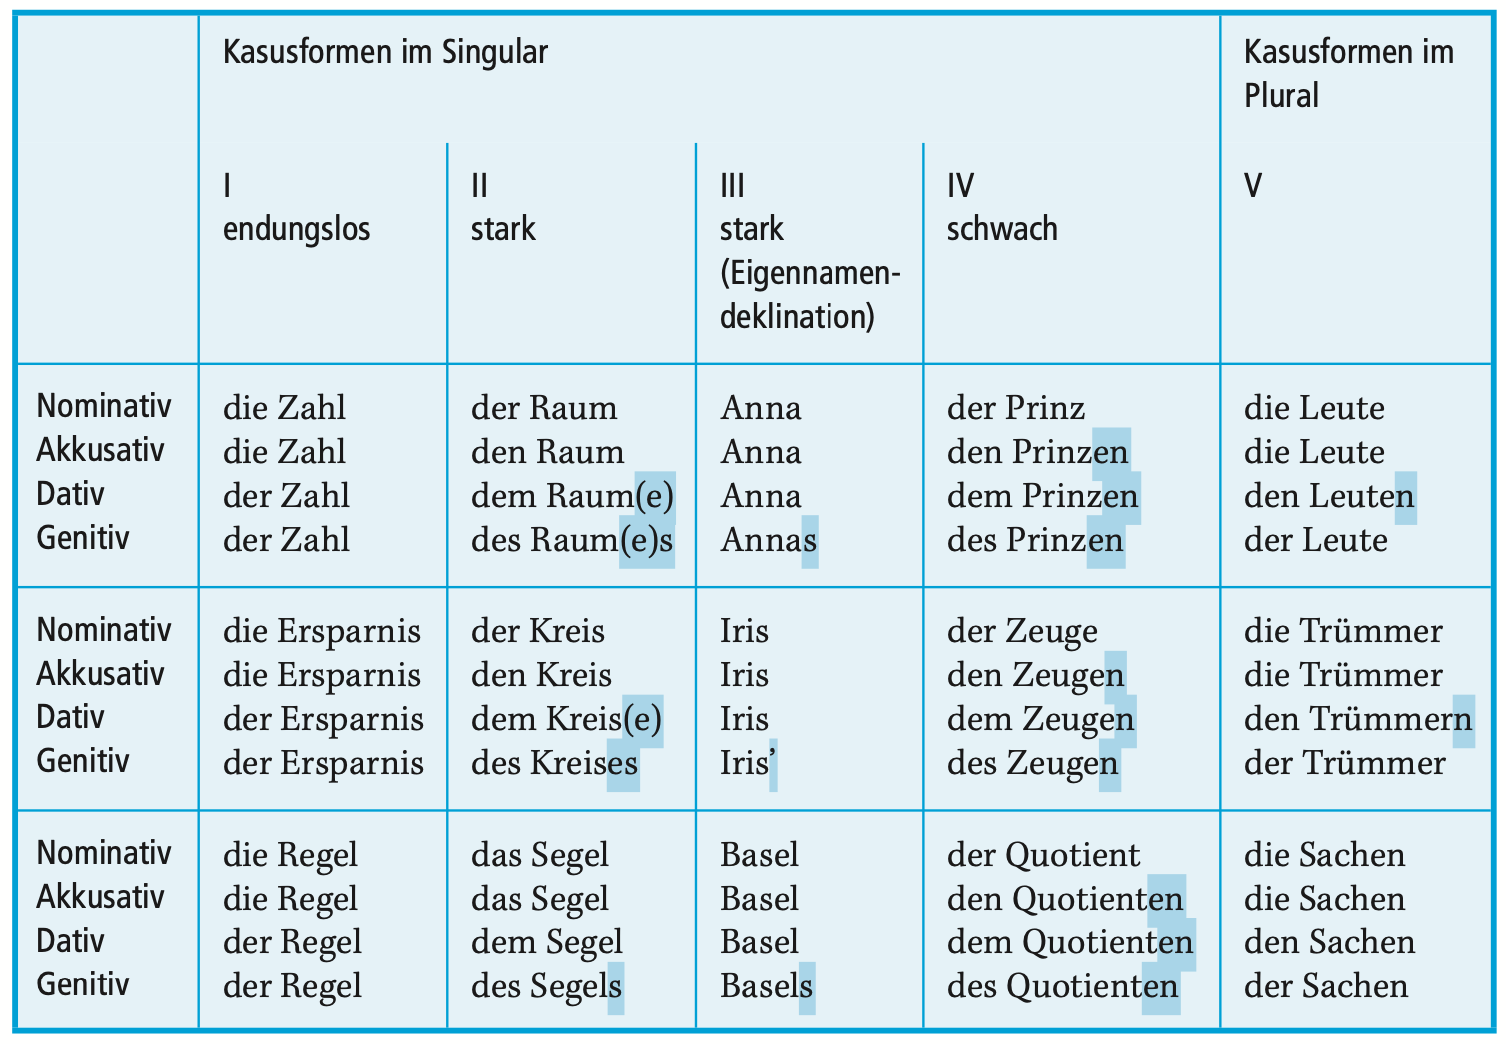
\includegraphics[scale=0.6]{kasus.png}
\end{figure}

\begin{itemize}
    \item K1:阴性单数 → Flexionsklasse I 
    \item K2:阳性/中性单数 → Flexionsklasse II
    \item K3:专有名词 + 无冠词 → Flexionsklasse III
    \item K4:阳性 + 有生命 + 复数以n结尾 → Flexionsklasse IV
    \item K5:复数 → Flexionsklasse V
\end{itemize}


\chapter{Pronomen/Artikle}
\begin{figure}[H]
    \centering
    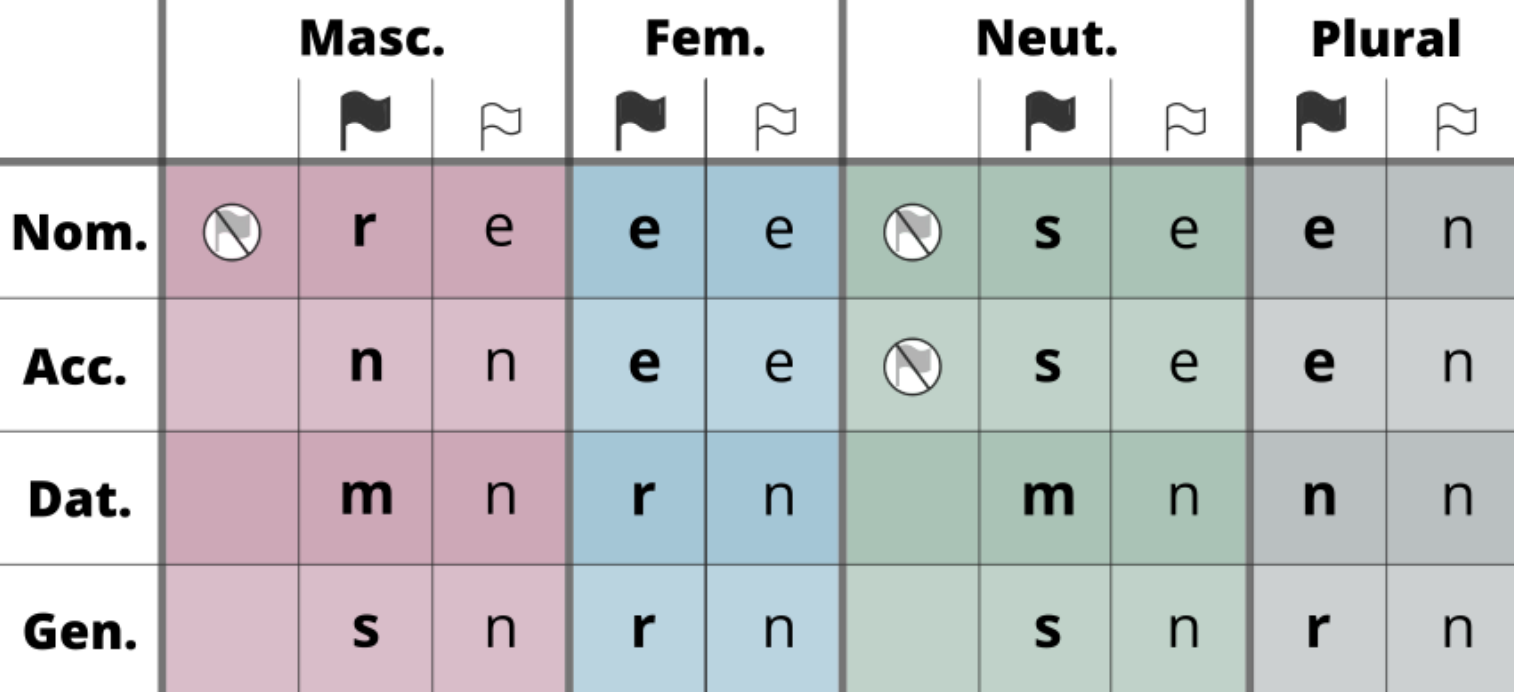
\includegraphics[scale=0.4]{dc.png}
\end{figure}
\section{Interrogative}
\begin{enumerate}
    \item 疑问词后可加genau oder ungefähr
    \begin{itemize}
        \item Wem genau hast du diesen Bericht geschickt
        \item An welcher Stelle genau stand der Wagen
        \item Wo stand der Wagen ungefähr
    \end{itemize}
    \item 疑问词后可加alles表示复数
    \begin{itemize}
        \item Mit wem alles sprechen eure Kinder
        \item Es ist toll, mit wem allem man sich hier austauschen kann
        \item Was steht alles im Bericht
    \end{itemize}
\end{enumerate}

\subsection{welch}
\begin{enumerate}
    \item Ausrufesätzen中,可使用无变格的welch和welch ein,表示was für ein
    \begin{itemize}
        \item Welch kluger Gedanke! (= Was für ein kluger Gedanke!)
        \item Welch ein Wunder! (= Was für ein Wunder!)
    \end{itemize}
    \item Fragesätzen中,welch和welch ein过时
    \begin{itemize}
        \item Wir erkundigten uns, welch brutaler Mensch / welch ein Mensch dies getan hatte
    \end{itemize}
\end{enumerate}


\subsection{wer/was}
\begin{enumerate}
    \item wessen作为形容词在名词前时,只表示与人相关联(谁的)
    \begin{itemize}
        \item Wessen Buch hast du denn mitgenommen
        \item Wessen Buch ich mitgenommen habe, ist meine Sache
    \end{itemize}
    \item wessen在问句中作为Genitivobjekt,可表示与事物/事实相关联
    \begin{itemize}
        \item Wessen erinnerst du dich? (= Welcher Personen / welcher Sachverhalte erinnerst du dich?)
        \item Wessen bedarfst du am meisten? (= Welcher Sachen bedarfst du am meisten?) 
    \end{itemize}
    \item was在口语中可作为副词使用,疑问句中表示warum,感叹句中表示wie
    \begin{itemize}
        \item Was bleibst du denn sitzen? Was hinkt er denn so? 
        \item Was ist der blöde
    \end{itemize}
\end{enumerate}

\subsection{Was für(ein)}
nach der Beschaffenheit, nach der Eigenschaft, nach einem Merkmal eines Wesens oder Dinges
\begin{enumerate}
    \item 作为冠词,für不改变其后名词Kasus
    \begin{itemize}
        \item Was für ein Auto fährst du
        \item Mit was für Leuten verkehrt sie denn so
        \item Was für einen Eindruck hast du
        \item Was hast du für einen Eindruck
    \end{itemize}
    \item 作为代词
    \begin{itemize}
        \item Was für einer bist denn du
    \end{itemize}
    \begin{enumerate}
        \item 作为代词指代复数、不可数名词单数时,ein替换为welch
        \begin{itemize}
            \item »In diesem Park stehen viele schöne Bäume.« »Was für welche?«
            \item Wir haben ausgezeichneten Wein getrunken.« »Was für welchen denn?«
        \end{itemize}
    \end{enumerate}
    \item 强调时,was放在句首,与für部分分开;vor allem bei der Frage nach Akkusativobjekten
    \begin{itemize}
        \item Was hast du für einen Eindruck
    \end{itemize}
    \item was an;an后名词都要变为dativ;bei Fragen nach dem Subjekt oder dem Akkusativobjek
    \begin{itemize}
        \item Was (alles) an Vorschlägen habt ihr eingereicht?
        \item Mir ist noch nicht ganz klar, was an Material wir benötigen
        \item Was (genau) an Vorräten ist noch da
        \item Was ist an Vorschlägen eingereicht worden
    \end{itemize}
    \item was von/aus;变格
    \begin{itemize}
        \item Was von diesen Sachen wird noch gebraucht
        \item Wer von diesen Kindern muss auch in den Ferien betreut werden
        \item Für wen von/aus dieser Klasse ist das bestimmt
    \end{itemize}
    \begin{enumerate}
        \item von部分作为Subjekts oder des Akkusativobjekts时可分
        \begin{itemize}
            \item Was wird von diesem Material noch gebraucht
            \item Wen (alles) kennst du von dieser Klasse
        \end{itemize}
    \end{enumerate}
\end{enumerate}

\section{Relative}
\subsubsection{Was/Wer}
\begin{figure}[H]
    \centering
    
\includegraphics[scale=0.5]{wer.png}
\end{figure}
was的dativ常替换为Pro-adverb
\begin{enumerate}
    \item 不涉及上一句中的某词
    \begin{itemize}
        \item ich kann mir denken, wen du meinst
        \item Was ich nicht 
    \end{itemize}
\end{enumerate}


\section{Indefinita}
\subsection{all}
\begin{enumerate}
    \item 可数名词all用复数(=sämtlich),不可数名词all用单数(=ganz, gesamt)
    \begin{itemize}
        \item Alle (= sämtliche) Bäume waren morsch
        \item Sie hat alles (= das ganze/gesamte) Geld verloren
    \end{itemize}
    \item all在定冠词前、dieser和jener前、Possessiven前可无格
    \begin{itemize}
        \item All der Fleiß war vergebens
        \item All mein Zureden half nichts
        \item  Mit all seinem Zauber ... All dieser Arbeit war er überdrüssig
    \end{itemize}
    \item all在Personalpronomen后
    \begin{itemize}
        \item sie alle, uns alle, wir andern alle, unser aller Leben
    \end{itemize}
    \item Nachstellung und Voranstellung
    \begin{enumerate}
        \item \emph{Nachstellung}: das alles, dies(es) alles, bei dem allem, mit diesem allem, diese alle
        \begin{enumerate}
            \item all在dem und diesem后的结尾-en有时会被替换为-em
        \end{enumerate}
        \item Voranstellung: alles das, alles dies, alles dieses, alle diese, mit allem diesem, bei allem dem
        \item Bei Voranstellung auch flexionslose Formen: all das, all dies, mit all diesem, all diese
        \begin{enumerate}
            \item  mit Zusammenschreibung:bei alldem
            \item Nebenform:bei alledem
        \end{enumerate}
    \end{enumerate}
\end{enumerate}

\subsection{ein, irgendein}
\begin{enumerate}
    \item ein,Indefinitpronomens;man, jemand, jedermann, Personalpronomen
    \begin{itemize}
        \item  Das ist einer! Nach den Aussagen eines (= jemandes), der dabei war... Er tut einem (= mir/uns/jeder- mann) wirklich leid
        \item Was soll einer (= ich, man, jemand) dazu schon sagen
    \end{itemize}
    \item irgendein, Indefinitpronomens und Artikelwort
    \begin{itemize}
        \item Irgendeiner wird es wissen
        \item Sie stammt aus irgendeinem Kaff in Niedersachsen
    \end{itemize}
\end{enumerate}

\subsection{ein bisschen/wenig/paar}
\begin{enumerate}
    \item Artikelwörter und pronominal;常无格
    \begin{itemize}
        \item Mit ein bisschen Nachdenken lassen sich alle Rätsel im Spiel lösen
        \item Auf der Suche nach ein wenig Wärme
        \item Aus ein paar geplanten Hüh- nern wurden 3000
    \end{itemize}
    \begin{enumerate}
        \item 但ein bisschen中的ein可作为不定冠词变格
        \begin{itemize}
            \item Mit einem bisschen Nachdenken kommst du auch sicher auf die Urheberin dieser Zeilen
        \end{itemize}
        \item bisschen可与定冠词、Demonstrativen、Possessiven连用,需要变格(kein可变可不变)
        \begin{itemize}
            \item Sechzig Jahre und kein bisschen leise
            \item Keinem bisschen Grün, keinem Haus, nur hin und wieder einem Auto begegnet man auf dieser Straße
            \item Mit diesem bisschen Druck bleibt das Personenschiff am Anlegeort stabil stehen
            \item Was wollen Sie eigentlich mit Ihrem bisschen Asthma
        \end{itemize}
        \item 作为代词,可用ein weniges这种形式
        \begin{itemize}
            \item Und vorher, also unbedingt vor Tagesanbruch, nimmt man ein weniges zu sich
        \end{itemize}
    \end{enumerate}
    \item ein bisschen和ein wenig可作为Gradadverbien和Gradpartikeln修饰谓词和形容词
    \begin{itemize}
        \item Bleib doch noch ein bisschen / ein wenig
        \item Das Brot war schon ein bisschen / ein wenig alt
    \end{itemize}
    \item Paar大写是名词,表示两个物品配对
    \begin{itemize}
        \item Jedes System wird mit einem Paar Ohrhörer geliefert
    \end{itemize}
\end{enumerate}

\subsubsection{einige, etliche}
(wie dieser flektiert)
\begin{enumerate}
    \item Die Pluralformen bezeichnen eine nicht allzu große Anzahl, die Singularformen eine nicht allzu große Menge
    \item 与hundert und tausend类数词连用,表示mehrere
    \begin{itemize}
        \item Es gibt doch einige Tausend Menschen
    \end{itemize}
    \item 与其他数词连用,表示不确定、大概
    \begin{itemize}
        \item Es waren so einige zwanzig
    \end{itemize}
\end{enumerate}

\subsection{-erlei}
(无变格)表示种类;Artikelwörter und Pronomen
\begin{itemize}
    \item derlei, mancherlei, vielerlei, solcherlei; einerlei, zweierlei, dreierlei, tausenderlei
\end{itemize}
\subsection{etwas (irgendetwas)}
(无变格)etwas/was,加强:irgendwas/irgendetwas
\begin{enumerate}
    \item Artikelwort und Pronomen;表示eine nicht näher bestimmte Menge oder Sache.
    \begin{itemize}
        \item Ich brauche etwas Geld
        \item Irgendetwas passiert immer
    \end{itemize}
    \begin{enumerate}
        \item 与so连用
        \begin{itemize}
            \item Irgend so etwas muss es gewesen sein
            \item Er ist so etwas wie ein Dichter
        \end{itemize}
    \end{enumerate}
    \item 作为程度副词,修饰谓词或形容词
    \begin{itemize}
        \item Ich bleibe noch etwas.
        \item Der Wagen bewegte sich etwas
        \item Heute ist es etwas wärmer
    \end{itemize}
\end{enumerate}


\subsection{genug, genügend}
\begin{enumerate}
    \item Artikelwort und Pronomen
    \begin{itemize}
        \item Ich habe genug herausgefunden
        \item Im Kühlschrank ist genügend Essbares
        \item Am Gemüse war nicht genug Salz
    \end{itemize}
    \item 程度副词
    \begin{itemize}
        \item Das Wasser war heiß genug / genügend heiß.
    \end{itemize}
\end{enumerate}

\subsection{irgend-}
\begin{enumerate}
    \item irgendetwas, irgendein, irgendjemand, irgendwelche, irgendwer, irgendwas (Außerdem bei Adverbien:) irgendwo, irgendwann
    \item irgend so ein Kerl, irgend so einer, irgend so etwas
\end{enumerate}


\subsection{jeder, jedweder, jeglicher und jedermann}

\subsection{jemand, niemand}
so、irgend加强语气
\begin{itemize}
    \item So jemand gehört hinter Schloss und Riegel
    \item Kennst du irgendjemand hier
\end{itemize}

\subsection{man}
Akkusativ:einen;Dativ:einem
\begin{itemize}
    \item Man (Nominativ) ärgert sich über so etwas
    \item So etwas ärgert einen (Akkusativ)
    \item So etwas geht einem (Dativ) nahe
\end{itemize}


\subsection{manch}
Artikelwort und Pronomen; eineunbestimmte,nichtsehrgroße Anzahl
\begin{enumerate}
    \item dieser flektiert
    \begin{itemize}
        \item Das haben schon manche gesagt
        \item Mancher Student ist so von einem vorzeitigen Abbruch des Studiums verschont geblieben
    \end{itemize}
    \item manch前gar, so, wie加强语气
    \begin{itemize}
        \item So mancher hat das schon gewollt, aber nie erreicht. Gar mancher steht lebendig hier
    \end{itemize}
    \item manch ein
    \begin{itemize}
        \item Manch ein Unternehmer versucht, auf diesem Weg der Lkw-Maut auszuweichen.
        \item Für manch einen kam die Entscheidung nicht mehr rechtzeitig
    \end{itemize}
    \item manch可无格直接出现在名词前
    \begin{itemize}
        \item Wir haben manch schönes Gespräch geführt
    \end{itemize}
\end{enumerate}


\subsection{meinesgleichen, deinesgleichen }
Indefinitpronomen;像……这样的人
\begin{itemize}
    \item Meinesgleichen handelt nicht so. Deinesgleichen haben wir nicht wieder gese- hen. Euresgleichen brauchen wir hier nicht
\end{itemize}


\subsection{nichts}
Artikelwort und Pronomen
\begin{itemize}
    \item In der Natur gibts ja auch nichts Rechteckiges
    \item 强调:Ich weiß gar nichts / ganz und gar nichts / überhaupt nichts
\end{itemize}

\subsection{solch}
Artikelwort/Pronomen und Adjektiv;
\begin{enumerate}
    \item 变格
    \begin{enumerate}
        \item 复数;口语形式:so, sone
        \begin{itemize}
            \item Wo kann ich solche Leute finden
            \item Aber ein Gutes hat es, dass es so Leute wie Sie und mich gibt
            \item Na ja, die kamen dann mit sonen Sprüchen wie
            \item Andy ist ja auch auf sone Leute wie dich angewiesen
        \end{itemize}
        \item 单数;常跟在不定冠词后
        \begin{itemize}
            \item Ich habe einen ungefähren Einblick, was ein solcher Künstler für eine Gage bekommt
        \end{itemize}
    \end{enumerate}
    \item 无格
    \begin{enumerate}
        \item 在不定冠词前:solch ein, so ein, irgend so ein(口语:so'n, irgend so'n)
        \begin{itemize}
            \item Dann wird es klar, wie klug und peinlich genau solch ein Künstler wie Wagner war
            \item Mit solch einer Jacke war der Unbekannte bekleidet
            \item Ich finde es sehr schade, dass ihr son Theater macht
            \item Ists erlaubt mit soner Jacke auch Motorrad zu fahren
            \item Nun läuft aber auch jeder Hansel mit so ei- ner Jacke rum
            \item beschichtet mit irgend so einer speziellen Oxidmischung
            \item Er gehört ja irgend soner konservativen religiösen Gemeinschaft an
        \end{itemize}
        \item 作为Gradpartikel修饰形容词;口语形式:so
        \begin{itemize}
            \item Selten hat ein solch dickes Buch meine Aufmerksamkeit mehr gefesselt als dieses
            \item Selten hat ein solch dickes Buch meine Aufmerksamkeit mehr gefesselt als dieses
        \end{itemize}
        \begin{enumerate}
            \item so可在不定冠词前
            \begin{itemize}
                \item Selbst so ein dickes Buch
            \end{itemize}
        \end{enumerate}
        \item 无格直接用在名词前
        \begin{itemize}
            \item warum ich ein solch Gefühl theils für Lieder der Wilden, theils für Ossian insonderheit habe
            \item Solch Verhalten kommt allerdings auch im Leben von Nicht-Alkoholikern vor
        \end{itemize}
    \end{enumerate}
    \item Pronomen
    \begin{enumerate}
        \item etwas solches = so etwas = so was(口语)
        \begin{itemize}
            \item Aber niemand konnte etwas solches beobachten
            \item Einfach toll, dass man so etwas beobachten kann
            \item Ich konnte auch schon so was beobachten
        \end{itemize}
        \item ein solcher = solch einer = so einer = so jemand 
    \end{enumerate}
\end{enumerate}

\subsection{unsereiner}
Indefinitpronomen
\begin{enumerate}
    \item 我们中的一员
    \item 像我们这样人
\end{enumerate}

\subsection{viel, wenig}
viel – mehr – meiste;wenig – weniger – wenigste (seltener: – minder – mindeste)
\begin{enumerate}
    \item viel, wenig, mehr, weniger的无格形式,用作Artikelwort und Pronomen
\end{enumerate}

\subsection{welch}
\begin{enumerate}
    \item welch,用作Indefinitpronomen,变格与dieser同;指代前文提到的「复数名词」或「不可数名词」
    \begin{itemize}
        \item Manchmal waren gar keine Zigaretten im Haus ... Albert musste am Automaten welche ziehen
        \item Räson annehmen kann niemand, der nicht schon wel- che hat
    \end{itemize}
    \item irgendwelcher,用作Artikelwort,少数作为Indefinitpronomen
    \begin{itemize}
        \item irgendwelches aufgelesene Zeug
        \item Irgendwelche haben mal damit angefangen, jemanden zu mobben
    \end{itemize}
    \item etwelch,用作Artikelwort
    \begin{itemize}
        \item Mit etwelchem Glück wurden wir vor dem Regen mit der Arbeit fertig
        \item Gibt es etwel- che besondere Tipps
    \end{itemize}
\end{enumerate}

\subsection{wer, was}
jemand, einer


\chapter{Adjektive}
\section{Gebrauch}
\subsection{Attributive}
\begin{enumerate}
    \item Fernstellung:名词在句首
    \begin{itemize}
        \item Reisen hat sie schon [viele] unternommen = Sie hat schon [viele Reisen] unternommen
        \item Kopfsalat bekommst du dort [ganz frischen] = Du bekommst dort [ganz frischen Kopfsalat]
    \end{itemize}
    \item elliptisch:删去重复名词保留形容词
    \begin{itemize}
        \item Die großen Fische fressen die kleinen (= die kleinen Fische)
        \item Das rote Lämpchen leuchtete konstant, das blaue (= das blaue Lämpchen) blinkte.
    \end{itemize}
\end{enumerate}




\subsubsection{Flektierte Formen, vorangestellt}
\begin{enumerate}
    \item 名词前有两个变格形容词时
    \begin{enumerate}
        \item 两个形容词都修饰名词时,用逗号隔开
        \begin{itemize}
            \item Der Chemiker führte weitere, erfolgreiche Versuche durch
        \end{itemize}
        \item 前一个形容词修饰后面的「形容词+名词」组合时,无逗号
        \begin{itemize}
            \item Der Chemiker führte weitere erfolgreiche Versuche durch
        \end{itemize}
    \end{enumerate}
\end{enumerate}

\subsubsection{Flektierte Formen, nachgestellt}

\begin{itemize}
    \item Gefährlich sind die Früchte, vor allem die unreifen
    \item Und Geister, gute wie schlechte
\end{itemize}

\subsubsection{Unflektierte Formen, vorangestellt}
\begin{enumerate}
    \item feste Verbindungen
    \begin{itemize}
        \item auf gut Glück
        \item ein halb Dutzend
    \end{itemize}
    \item Farbadjektive
    \item Ableitungen auf er
\end{enumerate}

\subsubsection{Unflektierte Formen, nachgestellt}

\begin{enumerate}
    \item Enge Nachträge
    \begin{itemize}
        \item Whisky pur; Forelle blau
        \item über Fußball brutal reden alle
    \end{itemize}
    \item Lockere Nachträge:加逗号,Adjektiv- bzw. Partizipphrasen
    \begin{itemize}
        \item Gewehrkugeln, groß wie Taubeneier und klein wie Bienen
        \item Die Sekretärin, müde und abgespannt, legt die Füße auf das Pult
        \item Die Wanderer, vom kalten Regen schon ganz durchgefroren, erreichten endlich ein Gasthaus
        \item Kathrin, vom langen Schwimmen schon ganz blau im Ge- sicht, stellte sich unter die Dusche
    \end{itemize}
    \begin{enumerate}
        \item 形容词/分词短语可与名词分开
        \begin{itemize}
            \item Müde und abgespannt legte die Sekretärin die Füße auf das Pult
            \item Kathrin stellte sich unter die Dusche, [vom langen Schwimmen schon ganz blau im Ge- sicht]
        \end{itemize}
    \end{enumerate}
\end{enumerate}



\subsection{Substantiviert}
\begin{enumerate}
    \item 与Attributive变格方式相同
    \item 语言与颜色形容词名词无变格
\end{enumerate}


\subsection{Prädikative}
指称名词
\begin{itemize}
    \item Anna legte das Buch aufgeklappt zur Seite
    \item Die Birnen lagen reif unter dem Baum
    \item Anna isst sie lieber gebraten
    \item Otto strich die Wand hellblau
    \item Der Lehrling feilte das Werkstück rund
    \item Die Politikerin bezeichnete den Vorschlag als unkonventionell
    \item Die Politikerin hielt den Vorschlag für unkonventionell
\end{itemize}


\subsection{Adverbial}
\begin{enumerate}
    \item 指称动词
    \begin{itemize}
        \item Die Kinder schrien laut
        \item Er singt entsetzlich
        \item Die Fans verhielten sich unauffäl- lig
    \end{itemize}
    \item 指称句子
    \begin{itemize}
        \item Rita kommt sicher noch
    \end{itemize}
    \item 指称其他形容词
    \begin{itemize}
        \item Es wehte ein entsetzlich/abscheulich kalter Wind
        \item Dies ist typisch niederdeutsch
    \end{itemize}
    \item 指称副词、介词、连词
    \begin{itemize}
        \item Das Dorf liegt tief unten. Sie sitzt weit oben
        \item Der Kontrollschacht befindet sich schräg neben dem Hintereingang
        \item Rund um den Brunnen gibt es viele nette Caf ́es und Bars
        \item Und das Ganze geschah, kurz nachdem Molly vom Verhältnis ihres Mannes zu Annamarie Scalli erfahren hatte.
    \end{itemize}
\end{enumerate}



\section{Komparation}

\subsection{Positiv}
\begin{enumerate}
    \item 相等
    \begin{enumerate}
        \item so/ebenso/genauso/gleich + 形容词 + (als) wie + 名词/句子/形容词
        \begin{itemize}
            \item Strecke a ist so/ebenso/genauso/gleich lang wie Strecke
            \item Renate rannte so/genauso schnell, wie wir erwartet hatten
            \item und bin so klug als wie zuvor
            \item Er ist so dumm wie faul
        \end{itemize}
        \item so + 形容词 + wie/als + möglich:尽可能……
        \begin{itemize}
            \item Fabiana wollte so lang wie möglich / so lang als möglich unter Wasser blei- ben
        \end{itemize}
    \end{enumerate}
    \item 不等
    \begin{enumerate}
        \item 程度副词 + so + 形容词 + wie/als
        \begin{itemize}
            \item Strecke a ist doppelt so lang wie Strecke b
            \item Diese Schachtel ist fast/mindestens/doppelt/dreimal so schwer wie jene
            \item Der zweite Oberton schwingt dreimal so schnell als der Grundto
        \end{itemize}
    \end{enumerate}
\end{enumerate}

\subsection{Komparativ}
\begin{enumerate}
    \item andere, niemand, keiner, nichts, umgekehrt, entgegengesetzt als
    \item 比较词
    \begin{enumerate}
        \item denn可作为比较词(veraltet) denn je:比以往更……
        \begin{itemize}
            \item Online-Tauschbörsen sind beliebter denn je
            \item Angesichts der begrenzten ärztlichen Möglichkeiten sind Mediziner weniger als Heiler denn als Berater gefragt
        \end{itemize}
        \item als wie可作为比较词(veraltet)
        \begin{itemize}
            \item geschwinder als wie der Wind
            \item Es ist hier anders als wie zu Hause
        \end{itemize}
    \end{enumerate}
    \item 比较级可通过程度词强化
    \begin{itemize}
        \item Die Strecke a ist \textbf{noch/etwas/viel/bedeutend/ungleich/erheblich} länger als die Strecke b
        \item Die Strecke a ist zehn Zentimeter länger als Strecke b
    \end{itemize}
    \item 否定比较级(较小程度)
    \begin{enumerate}
        \item weniger/minder
        \begin{itemize}
            \item Dieses Bild ist weniger schön als jenes
            \item In dem nicht minder fesselnden zweiten Teil des Romans
        \end{itemize}
        \item nicht weniger als……表示事物的完整
        \begin{itemize}
            \item Ich habe nicht weniger als 100 Euro dabei eingebüßt
        \end{itemize}
        \item nichts weniger als 表示否定
        \begin{itemize}
            \item Ich bin mit nichts weniger zufrieden als mit deinen Leistungen
        \end{itemize}
    \end{enumerate}
    \item 表示两形容词的程度不等:eher, mehr oder weniger
    \begin{itemize}
        \item Aline ist eher unkonzentriert als unsorgfältig
        \item Ich war mehr tot als lebendig. Alfons handelte weniger leichtsinnig als unüberlegt
    \end{itemize}
    \item 程度不断增加
    \begin{enumerate}
        \item immer + Komparativ
        \begin{itemize}
            \item Der Kater wurde immer dicker
        \end{itemize}
        \item Positiv + Komparativ
        \begin{itemize}
            \item Die Blicke werden tief und tiefer
        \end{itemize}
        \item Komparativ + Komparativ
        \begin{itemize}
            \item Ganz langsam sinkst du nun tiefer und tiefer in einen wunderschönen Zustand der absoluten Entspannung
        \end{itemize}
    \end{enumerate}
\end{enumerate}

\subsection{Superlativ}
\begin{itemize}
    \item Strecke d ist am längsten / die längste
\end{itemize}
\begin{enumerate}
    \item 比较的范围用Gentiv或von表示
    \begin{itemize}
        \item Strecke d ist am längsten / die längste von allen 
        \item Diese Kirche hat Europas größtes Zifferblatt / das größte Zifferblatt Europas / 
        
        das größte Zifferblatt von Europa
    \end{itemize}
    \item 强化最高级:aller-, alleraller-, weitaus, bei Weitem, denkbar
    \begin{itemize}
        \item die allerschönste, der allergrößte, das allerallerschönste, 
        
        weitaus der beste, bei Weitem der größte, in denkbar kürzester Frist
    \end{itemize}
    \item 最小程度用am wenigsten表示
    \begin{itemize}
        \item Dieses Bild ist am wenigsten schön
    \end{itemize}
    \item Elativ:不与其他对象比较,仅强调事物本身的极致属性
    \begin{enumerate}
        \item aufs + -ste
        \begin{itemize}
            \item Die Messungen wurden aufs Empfindlichste gestört
            \item Auch die kleinen Gäste werden aufs Beste unterhalten
        \end{itemize}
        \item 无变格
        \begin{itemize}
            \item Wir waren höchst erstaunt.
            \item Er nickte ihm ergebenst zu
        \end{itemize}
        \item sehr, höchst, äußerst, überaus, ungemein, besonders, erstaunlich, schrecklich, irre, furchtbar, ätzend + Positiv
        \item mehr als + Positiv
        \begin{itemize}
            \item Er ist mehr als durchtrieben
            \item Das ist eine mehr als leichtsinnige Auffassung
        \end{itemize}
    \end{enumerate}
\end{enumerate}

\chapter{Adverb}
\section{Bildung}
形容副词最高级
\begin{enumerate}
    \item am + sten(s)
    \begin{itemize}
        \item schnell: am schnellsten — schnellstens
    \end{itemize}
    \item aufs + ste
    \begin{itemize}
        \item aufs schönste, aufs beste, aufs freundlichste
    \end{itemize}
    \item -st
    \begin{itemize}
        \item baldigst, höflichst, möglichst, freundlichst
    \end{itemize}
\end{enumerate}

\section{Syntaktische Klasse}

\begin{figure}[H]
    \centering
    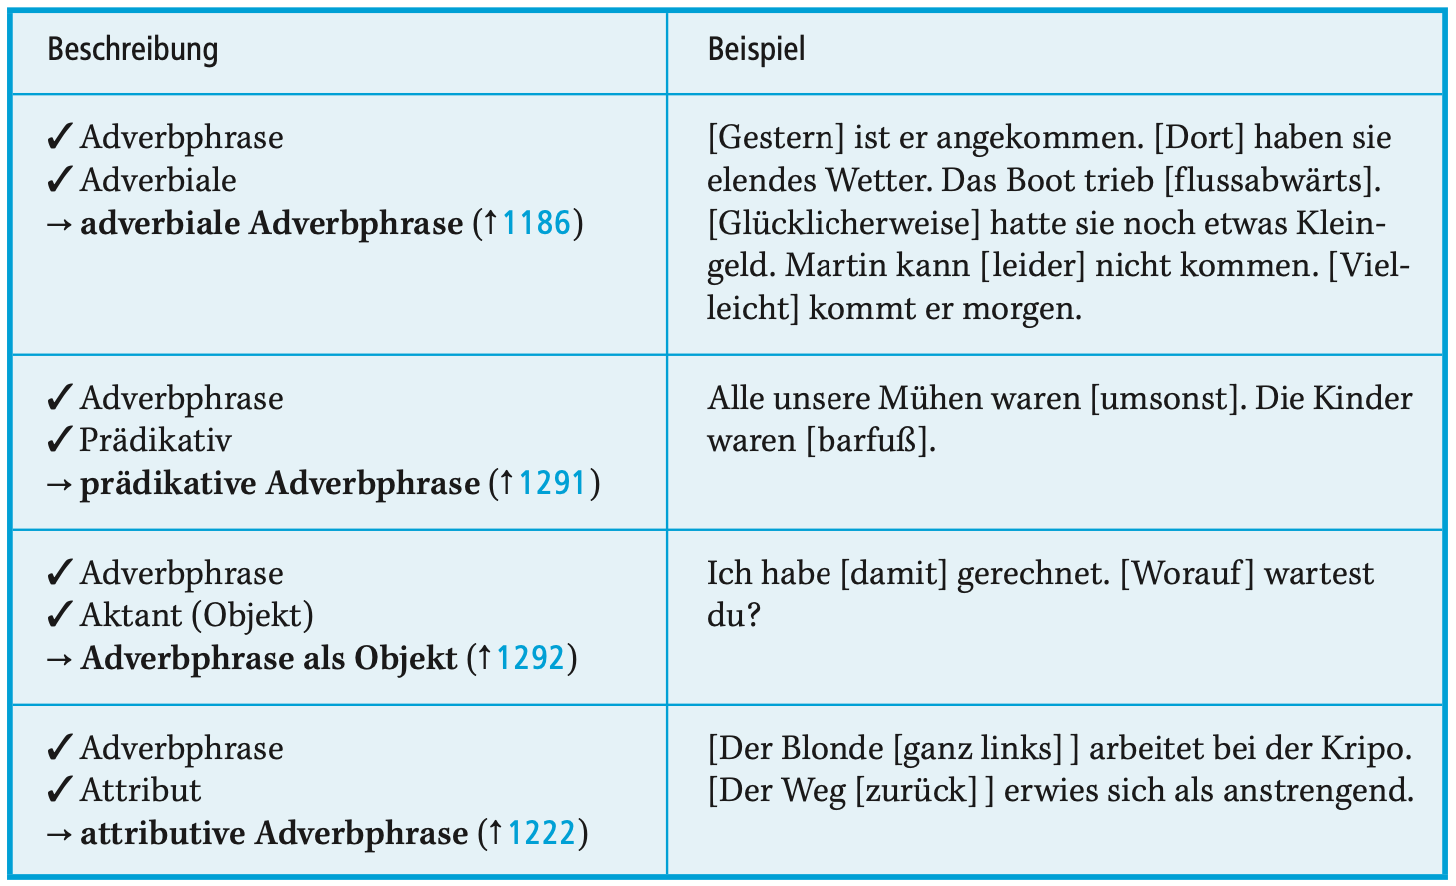
\includegraphics[scale=0.5]{adv.png}
\end{figure}

\section{Semantische Klassen}
Indefinitadverbien
\begin{enumerate}
    \item lokal: irgendwo, irgendwohin, irgendwoher, irgendworauf, irgendwodurch
    \item temporal: irgendwann, einmal, mal
    \item modal: irgendwie
    \item kausal (im weiteren Sinn; hier: final): irgendwozu (selten)
\end{enumerate}
n-Adverbien
\begin{enumerate}
    \item lokal: nirgends, nirgendwo, nirgendwohin, nirgendwoher
    \item temporal: nie, niemals
\end{enumerate}

Textadverbien:erstens, zweitens, einerseits, andererseits, ferner, 847 weiterhin, schließlich

\subsection{Lokaladverbien}
\subsubsection{Ortsadverbien}
hier, da, dort, draußen, drinnen, drüben, oben, unten, rechts, links, vorn, hinten, innen, außen, nirgends/nirgendwo, irgendwo, allseits, überall, allenthalben, mittendrin, darin, obenauf, wo

\subsubsection{Richtungsadverbien}
hierher, hierhin, dorther, dorthin, (von) überallher, irgendwohin, irgendwoher, überallhin, nirgendwohin, nirgendwoher, aufwärts, abwärts, vorwärts, rückwärts, seitwärts, heimwärts, heim, nach vorn/hintenloben/unten, beiseite, querfeldein, bergauf, bergab, weg, wohin, woher

\begin{itemize}
    \item Ortsadverbien与von(Herkunft)和nach(ziel)连用,可变为Richtungsadverbien
    \begin{itemize}
        \item Er kommt von drüben
        \item Er geht nach drüben
    \end{itemize}
\end{itemize}

\subsection{Temporaladverb}
\subsubsection{Zeitpunkt}

\begin{itemize}
    \item jetzt/nun/heute(正在), sofort/sogleich/gleich(立刻), bald/gleich/demnächst(马上/不久后), einst/einmal/dereinst(将来)
    
    \item soeben/vorhin(刚刚), gerade/eben(正在、刚刚), neulich/unlängst(不久前), einst/einmal/früher/eher/ehemals(以前)
    \item danach, da, darauf(hin), hinterher, nachher, fortan, seitdem, seither
    \item davor, vorher, zuvor
    \item indessen, unterdessen, mittlerweile, inzwischen:同时
    \item gestern, vorgestern, morgen, übermorgen, morgens, mittags, abends, nachts
\end{itemize}

\subsubsection{Zeitdauer}
immer, stets, lange, längst, zeitlebens

seither, bisher/bislang

tagsüber/nachts/wochenlang/monatelang/jahrelang

\subsubsection{Wiederholung}
manchmal, bisweilen, zuweilen, zeitweise, gelegentlich, oft, öfter, öfters, manchmal, mitunter, ab und zu

häufig, durchweg, mehrmals, nochmals

werktags, morgens, mittags, abends, nachts, sonntags, montags, vormittags, nachmittags, zweimal, dreimal


\subsection{Modaladverb}
ansatzweise, einigermaßen, etwa, halbwegs:有点

dermaßen:如此程度

fast, beinahe, geradezu, nachgerade, nahezu:几乎

schätzungsweise:大约

schlechthin, schlechterdings, Äußerst:absolutely, extremely

nebenbe:by the way

weitaus:more

zutiefst

vergebens, umsont:徒劳地

zudem, außerdem, obendrein, darüber hinaus

gleichwohl, trotzdem, nichtsdestotrotz, nichtsdestoweniger

\subsection{Kausaladverb}
-(et)wegen oder -halber
\begin{itemize}
    \item meinetwegen, deinetwegen, seinetwegen, ihretwegen
    \item gesundheitshalber, krankheitshalber, umständehalber, anstandshalber, sicherheitshalber, höflich- keitshalber, deutlichkeitshalber
\end{itemize}

\subsection{Interrogativadverb}
\begin{enumerate}
    \item lokal: wo, woher, wohin, wozwischen, woran usw.
    \item temporal: wann
    \item modal: wie(可与形容词连用)
    \begin{itemize}
        \item Er sagt nicht, wie oft er die Fenster putzt
    \end{itemize}
    \item kausal: warum, weshalb, weswegen, wieso
\end{enumerate}

\subsection{Relativadverb}
除了wann与Interrogativadverb同
\begin{itemize}
    \item Sie ist nach München gefahren, wohin er auch kommen will
    \item Es gibt nicht einen Grund, warum/weshalb/weswegen/ wieso man das anders machen sollte
    \item Sie besteht auf einer Entschädigung, worauf sie eigentlich keinen Anspruch hat
    \item Er staunt über (die Art), wie sie sich aus der Affäre zieht
    \item Es fand ein Konkurrenzkampf statt, wie man ihn bisher nicht kannte
\end{itemize}

\subsection{Pronominaladverb}
副词+介词, 元音间加r(darauf, worin), 口语中省略为drauf, drunter

\begin{enumerate}
    \item 现场指称deiktisch
    \begin{itemize}
        \item Sie schiebt den Karton darunter/hierunter
    \end{itemize}
    \item 回指前文anaphorisch:名词、名词短语、整个句子
    \begin{itemize}
        \item Sie fuhr den Wagen nicht in die Garage, sondern stellte ihn davor ab
    \end{itemize}
    \item 先行后指kataphorisch:指称从句关联词、不定式短语、整个从句
    \begin{itemize}
        \item Sie dachte nicht daran, aufzuräumen
        \item Sie hat nichts dagegen, den Vertrag zu verlängern
        \item Er tröstete sich damit, dass es wenigstens seinem Kind gut ging
        \item Sie überraschte ihre Schwester dabei, wie sie Geld abhob
        \item Es bleibt dabei: Wir reisen morgen ab
        \item Sie überraschte ihre Schwester dabei, wie sie Geld abhob
        \item Ich bin weiterhin dafür: Das Ehegattensplitting muss abgeschafft werden
    \end{itemize}
    \begin{enumerate}
        \item 指称Relativsatz时Pronominaladverb必须要拆开
        \begin{itemize}
            \item Du darfst über das (*darüber), was ich dir erzählt habe, nicht sprechen
            \item Du brauchst vor dem (*davor), was passieren wird, keine Angst zu haben
        \end{itemize}
    \end{enumerate}
    \item 当指称无生命物时用Pronominaladverb,指称有生命物时必须拆开(darunter und davon是例外)
    \begin{itemize}
        \item Ich warte auf den Auftrag→Ich warte darauf(*aufihn)
        \item Ich warte auf meinen Hund →Ich warte auf ihn (*darauf)
        \item Auf wen warten sie? -- Worauf warten sie?
        \item Vor wem hast du Angst? -- Wovor hast du Angst?
        \item der Arzt, vor dem du Angst hast -- etwas, wovor du Angst hast
    \end{itemize}
\end{enumerate}


\subsection{Konjunktionaladverb}
与Konjunktion的区别:Konjunktionaladverb可成为Vorfeld,但Konjunktion取消了Vorfeld成为link Satzklammer,随之导致finite verb的位置不同
\begin{figure}[H]
    \centering
    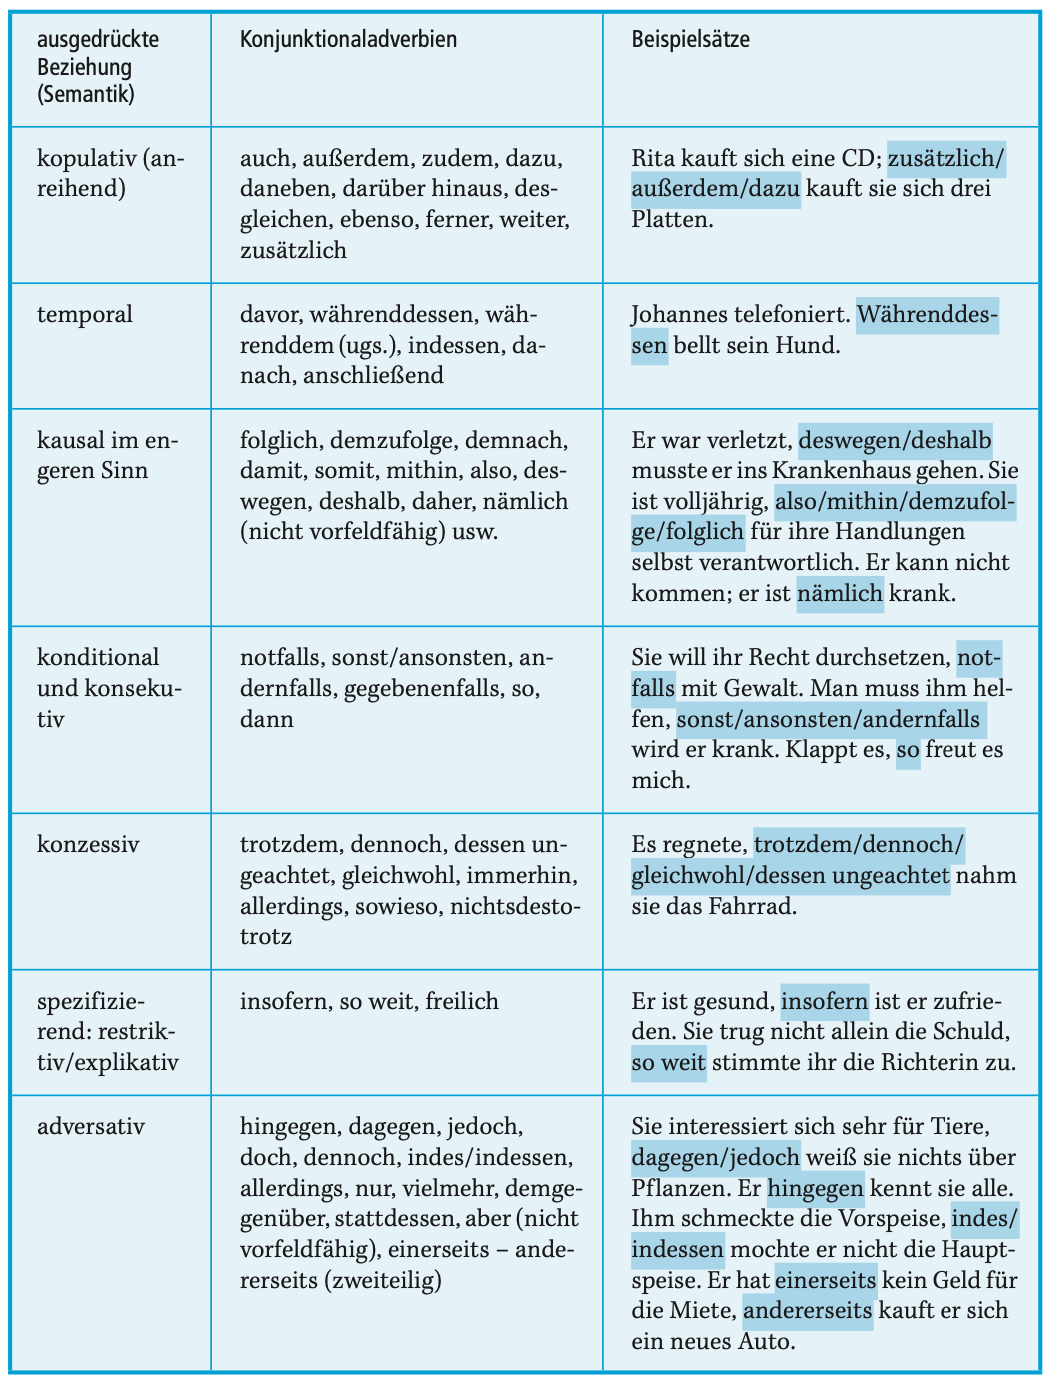
\includegraphics[scale=0.75]{ka.png}
\end{figure}

\begin{enumerate}
    \item immerhin
    \begin{enumerate}
        \item 表示尽管存在某些不足或限制,但仍有值得肯定的部分:至少、好歹
        \begin{itemize}
            \item Es ist nicht perfekt, aber immerhin besser als nichts
        \end{itemize}
        \item 提醒对方注意被忽视的事实:毕竟
        \begin{itemize}
            \item Immerhin habe ich dir geholfen, als du mich brauchtest
            \item Du solltest es besser wissen. Immerhin bist du Lehrer
        \end{itemize}
    \end{enumerate}
    \item notfalls/nötigenfalls:必要时,其他方法无效时的最后选择
    \begin{itemize}
        \item Nimm den Zug, notfalls ein Taxi
    \end{itemize}
    \item gegebenfalls
    \begin{itemize}
        \item Gegebenenfalls ist eine Genehmigung erforderlich(必要时)
        \item Bringen Sie Snacks mit, gegebenenfalls gibt es vor Ort nichts(以防、如果有情况发生)
    \end{itemize}
    \item ohnehin/sowieso:反正/无论如何,某事在任何情况下都成立或不需要特别考虑
    \begin{itemize}
        \item Ich gehe sowieso ins Fitnessstudio, da kann ich dich mitnehmen
        \item Das brauchen wir sowieso nicht.
        \item Die Entscheidung war ohnehin gefallen
    \end{itemize}
    \item jedenfalls
    \begin{itemize}
        \item Ich komme jedenfalls pünktlich(无论如何)
        \item Jedenfalls sollten wir es versuchen(至少)
    \end{itemize}
\end{enumerate}

\subsection{Kommentaradverb}
leider, bedauerlicherweise, dummerweise(不幸地)

allerdings, freilich(的确)

immerhin(至少好歹)

jedenfalls(至少、总之、无论如何)

anerkanntermaßen, bekanntermaßen(众所周知)

zugegebenermaßen(诚然)

seltsamerweise(奇怪的是), überraschenderweise, unerwarteterweise(出乎意料地)

kaum, möglicherweise, bestimmt/sicher(lich), vielleicht/Vermutlich, zweifellos, zweifelsohne

\chapter{Partikel}
与Adverb不同,Partikel不是Satzglieder,所以它不能单独出现在Vorfeld



\section{Gradpartikel}
wenig, etwas, einigermaßen, fast, ziemlich, recht, so, sehr, ausgesprochen, besonders, ungemein, überaus, ganz, äußerst, ungewöhnlich, vollkommen, zutiefst, höchst, zu

只与否定词连用:gar/überhaupt/beileibe nicht

与比较级或最高级连用:viel/weit/weitaus/nur noch

\section{Fokuspartikel}
Sogar/selbst/auch/besonders:even

einzig/nur/bloß/allein

Ausgerechnet:好巧不巧/偏偏

\section{Modalpartikel}

\subsection{Aussagesätzen}
\begin{enumerate}
    \item ja:强调共识
    \begin{itemize}
        \item Wie du ja weißt, liegt sein Vater im Krankenhaus
    \end{itemize}
    \item eben/halt/nun einmal:事情just就是如此(无奈接受)
    \begin{itemize}
        \item Das Leben ist halt/eben ungerecht
        \item Es ist nun einmal so
    \end{itemize}
    \item doch:反驳预期
    \begin{itemize}
        \item Weil das Leben doch ungerecht ist
    \end{itemize}
    \item schon:缓和肯定或部分让步,确实/倒是,终究/反正
    \begin{itemize}
        \item Das ist schon richtig, aber...
        \item Er wird schon kommen
        \item Was kann ich da schon ausrichten
    \end{itemize}
    \item auch:强调事实(的确)、无奈接受事实whatever
    \begin{itemize}
        \item Ich will auch ein Eis
        \item Das ist auch so
        \item Was du auch tust, es wird immer einer besser sein.
        \item Er muss auch immer recht haben
    \end{itemize}
\end{enumerate}


\subsection{Ausrufe}
\begin{enumerate}
    \item ja:之前以为是该事不是如此而惊讶
    \begin{itemize}
        \item Der Vortrag war ja interessant
    \end{itemize}
    \item aber/vielleicht:之前认为就是如此但是没想到是如此程度
    \begin{itemize}
        \item Der Vortrag war aber/vielleicht interessant
    \end{itemize}
    \item bloß/nur:究竟/到底
    \begin{itemize}
        \item Was hat sie sich bloß/nur dabei gedacht
    \end{itemize}
\end{enumerate}

\subsection{Wunschsätzen}
Konjunktiv II, doch/nur/bloß:要是……就好
\begin{itemize}
    \item Hättest du bloß nichts gesagt
    \item Wenn nur der Frühling bald käme
    \item Wenn er doch käme
\end{itemize}

\subsection{Aufforderung}
\begin{enumerate}
    \item ja/bloß:警告、威胁
    \begin{itemize}
        \item Mach ja/bloß das Fenster zu
    \end{itemize}
    \item schon/gefälligst:紧迫、不礼貌
    \begin{itemize}
        \item Mach schon/gefälligst das Fenster zu!
    \end{itemize}
    \item nur/ruhig:允许、尽管放心去
    \begin{itemize}
        \item Mach nur/ruhig das Fenster zu! 
    \end{itemize}
    \item doch/(doch/eben/gerade)mal/einfach:劝说、建议
    \begin{itemize}
        \item Halt’ eben mal die Leiter!
        \item Mach doch/mal/einfach das Fenster zu!
    \end{itemize}
    \item halt:妥协认命,那就去
    \begin{itemize}
        \item Dann mach halt das Fenster zu
    \end{itemize}
\end{enumerate}

\subsection{Fragesätzen}
\begin{enumerate}
    \item nicht:想得到对这件事肯定的回答
    \begin{itemize}
        \item Ist das Essen nicht hervorragend? (→ Ja.)
    \end{itemize}
    \item etwa/vielleicht:想得到对这件事否定的回答
    \begin{itemize}
        \item Ist das Essen etwa/vielleicht hervorragend? (→ Nein.)
    \end{itemize}
    \item denn
    \begin{itemize}
        \item Wie heißt du denn?(善意的好奇)
        \item Kannst du denn schwimmen?(询问)
    \end{itemize}
    \item auch
    \begin{itemize}
        \item Kannst du auch schwimmen
        \item Hast du auch die Tür abgeschlossen
    \end{itemize}
\end{enumerate}


\chapter{Präposition}
介词 + 名词、代词、形容词、副词

\section{Stellung}
\subsection{Prästellung}

\subsection{Prä- und Poststellung}

gegenüber, entlang, ausgenommen, einbegriffen, bar, wegen, gemäß, nach (im Sinn von ›gemäß‹ oder ›folgend‹), betreffend, entgegen, entsprechend, eingedenk, entlang, ungeachtet, zufolge

\subsection{Poststellung}

zuliebe, halber

\subsection{Zirkumposition}
um……willen, von……an/ab/aus/auf/wegen, auf……hin


\section{Verschmelzung}
\begin{enumerate}
    \item zum, zur, im, am, beim, vom; (auch:) ins, ans, aufs
    \item (dem, das)vorm, vors, hinterm, hinters, überm, übers, unterm, unters, fürs, durchs, ums
    \item (Akk. Sg. Mask.)vorn, hintern, übern, untern, fürn, durch’n, aufn
    \item Gesprochener Sprache
    \begin{enumerate}
        \item (Dat. Sg. Fem /Akk. Sg. Fem. und Akk. Pl.)
        \begin{itemize}
            \item an’n, an’er, an’e, in’n, in’er, in’e, von’n, von’er, von’e, durch’e, mit’er
        \end{itemize}
        \item (unbestimmten Artikel)
        \begin{itemize}
            \item auf ’nem, auf ’ner, auf ’nen, auf ’ne, auf ’n, mit ’ner, mit ’nem, nach ’nem, nach ’ner
        \end{itemize}
    \end{enumerate}
\end{enumerate}




\section{Liste}

\subsection{à(A)}
用于价格前
\begin{itemize}
    \item Ich möchte fünf Briefmarken a sechzig
\end{itemize}
\subsection{ab(D)}
\begin{enumerate}
    \item 表示时间/空间的起点(=von……ab/an)
    \begin{itemize}
        \item Der Zug fährt ab Berlin-Schönefeld
        \item Ab acht Uhr bin ich wieder zu Hause
    \end{itemize}
    \item 超过(=mit mehr als)
    \begin{itemize}
        \item Dieser Film ist für Jugendliche ab 14 Jahren erlaubt
        \item Körpergrößen ab einem Meter siebzig bezeichnet man als groß
    \end{itemize}
\end{enumerate}


\subsection{abzüglich(G)}
扣除……之后
\begin{itemize}
    \item Der Nettopreis beträgt 100 Euro, abzüglich der Steuern
\end{itemize}


\subsection{als(无格)}
\begin{enumerate}
    \item Spezifizierung(=in der Eigenschaft, Funktion)
    \begin{itemize}
        \item Er arbeitet als Schlosser in einem kleinen Betrieb.
    \end{itemize}
    \begin{enumerate}
        \item als后名词的Kasus与其Bezugwort的Kasus相同
        \begin{itemize}
            \item Er bezeichnet die Montage als den aufwendigsten Arbeitsprozeß
            \item Er sprach von der Montage als dem aufwendigsten Arbeitsprozeß
        \end{itemize}
        \item Bezugwort是Genitiv,若als后名词无冠词则其为Nominativ
        \begin{itemize}
            \item die Kosten der Montage als (aufwendigster) Arbeitsprozeß
        \end{itemize}
    \end{enumerate}
    \item 比较, Ungleichheit im Vergleich;在形容词/副词后
    \begin{itemize}
        \item Er spielt anders als sein Gegner
    \end{itemize}
\end{enumerate}
\subsection{an(D/A)}
\begin{enumerate}
    \item Lokal
    \begin{enumerate}
        \item (D)Nicht zielgerichtet
        \begin{itemize}
            \item Der Schrank steht an der Wand
            \item Die Lampe hängt an der Decke
            \item Wir sitzen am Tisch
            \begin{figure}[H]
                \centering
                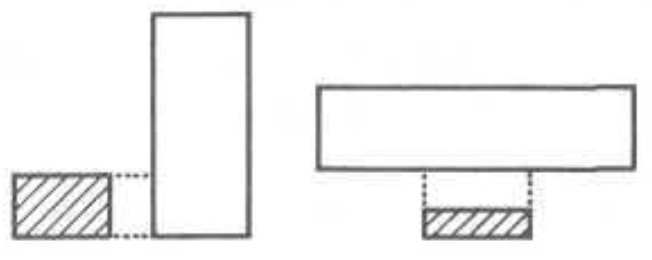
\includegraphics[scale=0.3]{an1.png}
            \end{figure}
        \end{itemize}
        \item (A)zielgerichtet
        \begin{itemize}
            \item Sie schieben den Schrank an die Wand
            \item Er hängt die Lampe an die Decke
            \item Wir setzen uns an den Tisch
            \begin{figure}[H]
                \centering
                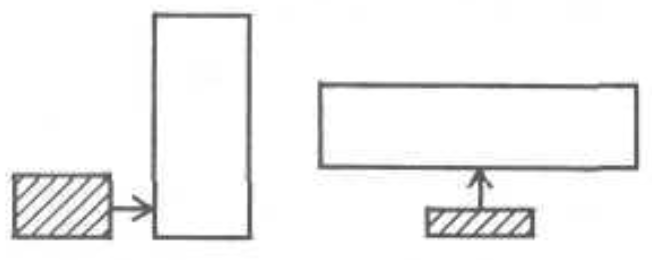
\includegraphics[scale=0.3]{an2.png}
            \end{figure}
        \end{itemize}
        \item (D)Geographisch 紧挨着;在山/水的名词前
        \begin{itemize}
            \item Halle an der Saale
            \item Köln am Rhein
        \end{itemize}
    \end{enumerate}
    \item (D)Temporal;在日期前
    \begin{enumerate}
        \item 月份前用in,除非是一月中的具体日子
        \begin{itemize}
            \item im Dezember1970
            \item am 31. Dezember 1970
        \end{itemize}
    \end{enumerate}
\end{enumerate}

\subsection{anlässlich}
(=während, bei)
\begin{itemize}
    \item Anlässlich seines Geburtstags veranstalten wir eine Feier
    \item Anlässlich der Konferenz wurden neue Richtlinien vorgestellt
\end{itemize}

\subsection{angesichts(G)}
鉴于(=wegen)
\begin{itemize}
    \item Angesichts der hohen Kosten müssen wir sparen
\end{itemize}

\subsection{anstelle(G)}
=anstatt


\subsection{auf(D/A)}
\begin{enumerate}
    \item Lokal 有接触
    \begin{enumerate}
        \item (D)Nicht zielgerichtet
        \begin{itemize}
            \item Das Buch liegt auf dem Tisch
            \begin{figure}[H]
                \centering
                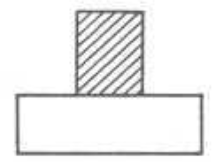
\includegraphics[scale=0.3]{auf1.png}
            \end{figure}
        \end{itemize}
        \item (A)zielgerichtet
        \begin{itemize}
            \item Sie legt das Buch auf den Tisch
            \begin{figure}[H]
                \centering
                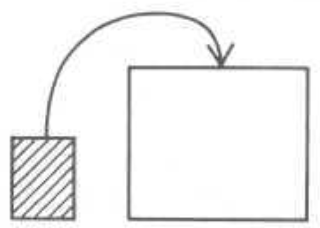
\includegraphics[scale=0.3]{auf2.png}
            \end{figure}
        \end{itemize}
    \end{enumerate}
    \item Final-Lokal;用于表示部门、机构的名词前
    \begin{enumerate}
        \item (D)Nicht zielgerichtet
        \begin{itemize}
            \item Sie kauft auf dem Postamt Briefmarken.
        \end{itemize}
        \item (A)zielgerichtet
        \begin{itemize}
            \item Sie geht auf das Postamt
        \end{itemize}
    \end{enumerate}
    \item Temporal
    \begin{enumerate}
        \item (D)Gleichzeitigkeit. Zeitdauer(=bei, während)
        \begin{itemize}
            \item Auf der Wanderung sahen wir verschiedene Wildtiere
            \item Auf dem Kongreß sprachen auch mehrere ausländische Vertrete
        \end{itemize}
        \item (A)Gleichzeitigkeit. Bevorstehende festgelegte Zeitdauer;用于前有数词的时间词(Woche, Monat, Jahrzehnt)前
        \begin{itemize}
            \item Sie ist auf drei Monate ins Ausland gefahren
            \item Die Strecke ist auf längere Zeit gesperrt
        \end{itemize}
        \begin{enumerate}
            \item 如果前无数词,时间词后跟hinaus(fak.)
            \begin{itemize}
                \item Der Betrieb ist auf Monate (hinaus) ausgelastet
            \end{itemize}
        \end{enumerate}
    \end{enumerate}
    \item Modal
    \begin{enumerate}
        \item (A)尺度;尺寸词后跟genau(fak./obl.)
        \begin{itemize}
            \item Er arbeitet auf den Zentimeter genau
            \item Er kommt auf die Minute (genau)
        \end{itemize}
        \item (A)程度(最高级);auf das/aufs + Superlativ
        \begin{itemize}
            \item Er arbeitet auf das genaueste
            \item Wir grüßen Sie aufs herzlichste
        \end{itemize}
        \item (无格)Steigende Wiederholung
        \begin{itemize}
            \item Tropfen auf Tropfen rann aus dem Wasserhahn
        \end{itemize}
        \item (无格)在语言名称前
        \begin{itemize}
            \item Er hat ihr das Kompliment auf englisch gemacht
        \end{itemize}
        \item auf einmal(=gleichzeitig);不能用于句首
        \begin{itemize}
            \item Er wollte alles auf einmal schaffen
        \end{itemize}
        \begin{enumerate}
            \item auf einmal表示「突然」时,可用于句首
            \begin{itemize}
                \item Auf einmal konnte sie ihn nicht mehr sehen
            \end{itemize}
        \end{enumerate}
    \end{enumerate}
    \item (A)Distributiv每个/逐个/分别
    \begin{itemize}
        \item Von diesem Medikament muß man 3 Tropfen auf ein Glas Wasser einnehmen
        \item Auf ein Kilo Mehl rechnet man 30 Gramm Hefe
    \end{itemize}
    \item (A)Kasual
    \begin{enumerate}
        \item 若auf后名词无冠词,则在其后加hin(fak.)
        \begin{itemize}
            \item Er las das Buch auf Anregung seines Professors (hin).
        \end{itemize}
        \item 若auf后名词有冠词,则在其后加hin(obl.)
        \begin{itemize}
            \item Er korrigierte einige Stellen im Vortrag auf die Kritik seines Freundes hin
        \end{itemize}
    \end{enumerate}
\end{enumerate}
\subsection{aus(D)}
\begin{enumerate}
    \item Lokal 出
    \item Kausal,无冠词
    \begin{itemize}
        \item Er arbeitet aus Überzeugung mit
        \item Er half ihr aus Mitleid
    \end{itemize}
    \begin{enumerate}
        \item aus表原因时主体做出有意识的动作;vor表原因时主体做出无意识(情不自禁)的动作
        \begin{itemize}
            \item vor Freude lachen, vor Schmerzen schreien, vor Kälte zittern, vor Hunger sterben
        \end{itemize}
    \end{enumerate}
    \item Modal 组成的材质(=von)
    \begin{itemize}
        \item Ein Haus aus Glas, Beton und Aluminium wird gebau
    \end{itemize}
    \item 从Lokal引申来的比喻义;表示状态改变
    \begin{itemize}
        \item Er hat lange nicht gespielt, er ist ganz aus der Übung gekommen.
    \end{itemize}
\end{enumerate}
\subsection{außer(D)}
\begin{enumerate}
    \item Restriktiv 除了,Gegenüberstellend einer Gesamtheit;常与alle, immer, niemand等总括词连用(=bis auf, mit Ausnahme von)
    \begin{itemize}
        \item Außer ihrem Zwillingsbruder waren alle Geschwister zur Geburts- tagsfeier gekommen.
        \item Außer dem Kind war niemand in der Wohnung.
    \end{itemize}
    \item Kopulativ 除了……还有, Gegenüberstellend einer Nicht-Gesamtheit;常与noch, auch, nur(noch)连用(=neben)
    \begin{itemize}
        \item Außer ihrem Zwillingsbruder waren noch zwei Brüder und eine Schwester gekommen.
        \item Außer Büchern werden dort auch Papier- und Schreibwaren ver- kauft
    \end{itemize}
    \item Lokal 不属于某一领域;无冠词(=außerhalb)
    \begin{itemize}
        \item Nach wenigen Minuten war das Boot außer Sichtweite
    \end{itemize}
    \item Modal 状态改变;无冠词
    \begin{itemize}
        \item Die Maschine war außer Betrieb
    \end{itemize}
\end{enumerate}
\subsection{außerhalb(G)}
\begin{enumerate}
    \item Lokal 不属于某一领域
    \begin{itemize}
        \item Die Garage befindet sich außerhalb des Wohnhauses
    \end{itemize}
    \item Temporal 不属于特定时间段
    \begin{itemize}
        \item Kommen Sie bitte außerhalb der Arbeitszeit
    \end{itemize}
    \item 比喻义(=jenseits)
    \begin{itemize}
        \item Er beschäftigt sich gern mit Dingen, die außerhalb seines Fachgebietes liegen
    \end{itemize}
\end{enumerate}

\subsection{bei(D)}
\begin{enumerate}
    \item Lokal
    \begin{enumerate}
        \item 紧挨着(= vor, hinter, über, unter, neben)
        \begin{itemize}
            \item Er saß bei seinen Freunden
            \item Das Haus steht bei einem Springbrunnen
        \end{itemize}
        \item Geographisch 附近
        \begin{itemize}
            \item In Markkleeberg bei Leipzig finden landwirtschaftliche Ausstel- lungen statt
        \end{itemize}
        \item 政经/个人领域
    \end{enumerate}
    \item Temporal
    \begin{enumerate}
        \item Gleichzeitigkeit. Zeitdauer(=auf, während)
        \begin{itemize}
            \item Beim Essen soll man nicht sprechen
        \end{itemize}
        \item Gleichzeitigkeit. Zeitpunkt(=mit)
        \begin{itemize}
            \item Beim Eintritt des Dozenten wurde es still
        \end{itemize}
    \end{enumerate}
    \item Konditional;多无冠词
    \begin{itemize}
        \item Bei Regen fällt die Veranstaltung aus
        \item Die Notbremse darf nur bei Gefahr gezogen werden
        \item Bei Glatteis ist besondere Vorsicht erforderlich
    \end{itemize}
\end{enumerate}

\subsection{betreffs/betreffend(G)}
关于,就……而言
\begin{itemize}
    \item Betreffs Ihrer Anfrage teilen wir Ihnen mit
\end{itemize}

\subsection{bezüglich}
关于,就……而言



\subsection{behufs(G)}
Final
\begin{itemize}
    \item Behufs der Klärung dieser Angelegenheit
\end{itemize}


\subsection{binnen(D)}
Temporal Gleichzeitigkeit. Begrenzte Zeitdauer;在数词前
\begin{itemize}
    \item Wir müssen die Arbeit binnen einem Monat (eines Monats) abschließen
    \item Der Exportauftrag ist binnen sechs Monaten zu erfüllen
\end{itemize}
\subsection{bis(A)}
\begin{enumerate}
    \item Lokal Strecke mit Angabe des Endpunktes
    \begin{enumerate}
        \item Geographisch 空间副词/地名前;双介词(fak.)且无冠词
        \begin{itemize}
            \item Er fuhr von Leipzig bis (nach) Weimar
            \item Bis (nach) dort drüben sind es knapp zehn Meter
        \end{itemize}
        \item 在其他方向词前;双介词(obl.)且有冠词
        \begin{itemize}
            \item Das Auto fuhr bis vor das Hotel
            \item Der Bus fuhr bis in das Stadion
        \end{itemize}
    \end{enumerate} 
    \item Temporal Zeitdauer mit Angabe des Endpunktes
    \begin{enumerate}
        \item 在时间副词/小时/年份前;无冠词(obl.)
        \begin{itemize}
            \item Bis 1945 lebte der Dichter in der Emigration
            \item Ich warte bis 12 Uhr
        \end{itemize}
        \item 在星期/月份/日期前;无冠词或双介词zu + 有冠词
        \begin{itemize}
            \item Bis (zur) Mitte der Woche hat sie Zeit
            \item Bis (zum nächsten) nächstes Jahr will er mit seiner Arbeit fertig sein
            \item Bis (zum) 1. September haben die Kinder Schulferien
        \end{itemize}
        \item 在其他时间词前;双介词zu(obl.) + 有冠词
        \begin{itemize}
            \item Bis zum vorigen Jahrhundert herrschte in Teilen Europas die Leibeigenschaft
            \item Der zweite Weltkrieg dauerte bis zum Jahr 1945
            \item Bis zu den Ferien muß ich noch viel erledigen
        \end{itemize}
    \end{enumerate}
    \item Modal 程度/尺度,最大限度;双介词(obl.)
    \begin{itemize}
        \item Sie marschierten bis zur Erschöpfung
        \item In dem Aufsatz ist alles bis ins letzte durchdacht
        \item Das Kino war bis auf den letzten Platz besetzt
        \begin{itemize}
            \item bis auf包含双重意思:最后一个座位仍空着(ausschließlich)/没有座位空着(einschließlich)
        \end{itemize}
    \end{itemize}
    \item Temporal/Modal 不确定的程度/时间;用于两数词之间表示限制;无冠词(obl.)
    \begin{itemize}
        \item Die Temperatur soll morgen 3 bis 8 Grad betragen
        \item Die Operation dauert zwei bis drei Stunden
    \end{itemize}
\end{enumerate}
\subsection{dank (D/G)}
Modal. Instrumental(=durch)
\begin{itemize}
    \item Dank seinem Fleiß bestand er die Prüfung
    \item Dank seines raschen Handelns wurde die Ertrinkende gerettet.
\end{itemize}
\subsection{diesseits(G)}
Lokal 界限
\begin{itemize}
    \item Weil keine Brücke zu finden war, mußten wir diesseits des Flusses bleiben
\end{itemize}
\subsection{durch(A)}
\begin{enumerate}
    \item Lokal 运动穿过该范围或在范围内
    \begin{itemize}
        \item Er sieht durch das Fernrohr
        \item Sie geht durch die Tür
        \item Wir bummeln durch die Stadt
        \begin{figure}[H]
            \centering
            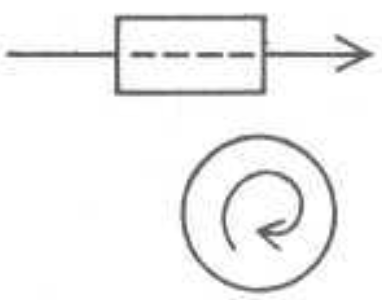
\includegraphics[scale=0.3]{durch.png}
        \end{figure}
    \end{itemize}
    \item Agens(=von)
    \begin{itemize}
        \item Amerika wurde durch Kolumbus entdeckt
    \end{itemize}
    \begin{enumerate}
        \item 名词短语中,durch紧挨genitiv或von短语后(此时不用von)
        \begin{itemize}
            \item die Entdeckung Amerikas durch Kolumbus
            \item die Entdeckung von Amerika durch Kolumbus
        \end{itemize}
    \end{enumerate}
    \item Modal. Instrument, Mittel, Vermittler(=mit, per)
    \begin{itemize}
        \item Sie versenkten das Schiff durch ein Torpedo
        \item Das Schiff wurde durch ein Torpedo versenkt
    \end{itemize}
    \begin{enumerate}
        \item 当durch同时可被解释为Agens和Vermittler时,表Agens时用von(不用durch),表Vermittler时用durch
        \begin{itemize}
            \item Der Brief wurde ihr durch einen Boten geschickt(der Bote ist Vermittler)
            \item Der Brief wurde ihr von einem Boten geschickt(der Bote ist Agens)
        \end{itemize}
    \end{enumerate}
    \item Temporal Gleichzeitigkeit, Begrenzte Zeitdauer;只以hindurch形式出现在名词后(Fak.)
    \begin{itemize}
        \item Sie arbeiteten die ganze Nacht (hindurch)
    \end{itemize}
    \item 从Lokal引申来的比喻义
    \begin{itemize}
        \item Durch die Diskussion zog sich ein Gedanke wie ein roter Faden
    \end{itemize}
\end{enumerate}

\subsection{entgegen(D)}
Adversativ;In Prä- oder Poststellung
\begin{itemize}
    \item Entgegen dem Befehl (dem Befehl entgegen) verließ er seinen Posten.
\end{itemize}

\subsection{entlang(A/D)}
\begin{enumerate}
    \item Lokal Parallelverlauf;A in Poststellung, seltener D in Post- oder Prästellung;(=neben, parallel zu, längs)
    \begin{itemize}
        \item Den Weg entlang (dem Weg entlang / entlang dem Weg) stehen hübsche Wochenendhäuser
        \item Der Weg führt den Bach (dem Bach) entlang
        \begin{figure}[H]
            \centering
            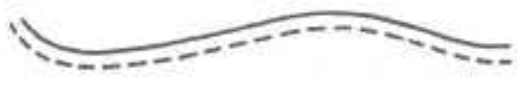
\includegraphics[scale=0.3]{entlang1.png}
        \end{figure}
    \end{itemize}
    \item Lokal 运动动词表示的位置变化;A in Poststellung
    \begin{itemize}
        \item Das Schiff fährt den Fluß entlang
        \item Wir wandern die Straße entlang
        \begin{figure}[H]
            \centering
            
\includegraphics[scale=0.3]{entlang2.png}
        \end{figure}
    \end{itemize}
\end{enumerate}

\subsection{für(A)}
\begin{enumerate}
    \item 目的
    \begin{itemize}
        \item Das Auto benötigt für die Bewältigung dieser Strecke eine Stunde
        \item Sie hat Wanderschuhe für den Urlaub gekauft
    \end{itemize}
    \item Bezugspunkt
    \begin{itemize}
        \item Er arbeitet gern für die Mathematik
        \item Seine Krankheit war für den Arzt neu
    \end{itemize}
    \item Modal
    \begin{enumerate}
        \item Komparativ(=im Hinblick auf, im Vergleich zu)
        \begin{itemize}
            \item Für sein Alter ist das Kind gut entwickelt
            \item Für die kurze Zeit seines Klavierunterrichts spielt er schon recht gut
        \end{itemize}
        \item (无格)Steigende Wiederholung
        \begin{itemize}
            \item Schritt für Schritt ging er vorwärts
        \end{itemize}
    \end{enumerate}
    \item Ersatz, Austausch(=statt)
    \begin{itemize}
        \item Für seinen Wagen bekam er nur wenig Geld
        \item Da er kein Geld bei sich hatte, habe ich für ihn bezahlt
    \end{itemize}
    \item Temporal. Gleichzeitigkeit. Begrenzte Zeitdauer(=auf)
    \begin{itemize}
        \item Für einen Tag herrschte Arbeitsruhe
        \item Das ist alles für diesmal
    \end{itemize}
    \item distributiv
    \begin{itemize}
        \item Sie kaufte zwei Kilo Äpfel für drei (zu drei) Mark
    \end{itemize}

    \begin{enumerate}
        \item 双重意思;加à, je, pro可只表示eigentlich distributive
        \begin{itemize}
            \item Ein Kilo Äpfel kostet drei Mark(eigentlich distributive Bedeutung)
            \item Zwei Kilo kosten drei Mark(summarische Bedeutung)
        \end{itemize}
    \end{enumerate}
\end{enumerate}

\subsection{gegen(A)}
\begin{enumerate}
    \item Lokal. Zielgerichtet
    \begin{enumerate}
        \item Vor statischem Ziel
        \begin{itemize}
            \item Das Auto ist gegen einen Baum gefahren
            \item Er schlug mit der Faust gegen die Tür
            \item Er stand mit dem Rücken gegen das Licht
            \begin{figure}[H]
                \centering
                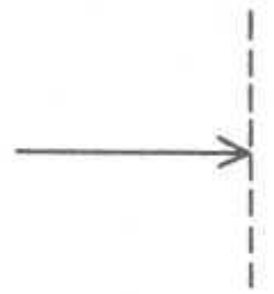
\includegraphics[scale=0.3]{gegen.png}
            \end{figure}
        \end{itemize}
        \item Vor dynamischem Ziel
        \begin{itemize}
            \item Er ruderte gegen den Strom
        \end{itemize}
    \end{enumerate}
    \item Adversativ
    \begin{enumerate}
        \item Relation. (= im Gegensatz zu)
        \begin{itemize}
            \item Gegen seinen Bruder ist er klein
            \item Gegen gestern ist es heute kalt
        \end{itemize}
        \item 从Lokal引申来的比喻义
        \begin{itemize}
            \item Er hat gegen das Gesetz verstoßen
            \item In der Diskussion hatte er alle gegen sich.
            \item Wir sind gegen Feuer und Diebstahl versichert.
        \end{itemize}
    \end{enumerate}
    \item Modal/Temporal. 不确定的时间
    \begin{itemize}
        \item Der Zug kommt gegen 19 Uhr an
        \item Er ist gegen Morgen gestorben
    \end{itemize}
\end{enumerate}

\subsection{gegenüber(D)}
Prä- und Poststellung. Bei Personenbezeichnungen vorwiegend, bei Personalpronomina immer Poststellung.
\begin{enumerate}
    \item Lokal 另一边
    \begin{itemize}
        \item Gegenüber dem Internat (dem Internat gegen- über) befindet sich ein Krankenhaus.
        \item Ihm gegenüber saß der Direktor
        \begin{figure}[H]
            \centering
            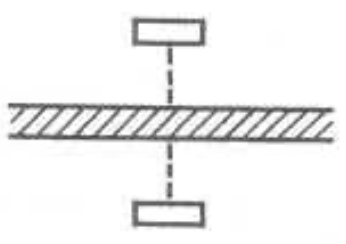
\includegraphics[scale=0.3]{gegenu.png}
        \end{figure}
    \end{itemize}
    \item Modal
    \begin{enumerate}
        \item Komparativ 比较
        \begin{itemize}
            \item Gegenüber einer Dampflok hat eine Diesellok viele Vorzüge.
            \item Gegenüber einem Zweitakter ist ein Viertakter ökonomischer.(与形容词比较级连用)
        \end{itemize}
        \item 对待某人的行为/态度
        \begin{itemize}
            \item Alten Menschen gegenüber soll man immer hilfsbereit sein
            \item Ich habe ihm gegenüber Hemmungen
        \end{itemize}
    \end{enumerate}
\end{enumerate}

\subsection{gemäß(D)}
Modal 按照,相符,根据;Poststellung, seltener Prä-stellung
\begin{itemize}
    \item Die Maschine wurde den Anweisungen gemäß (gemäß den Anwei- sungen) zusammengesetzt
\end{itemize}
\begin{enumerate}
    \item gemäß, laut, nach, zufolge区别
    \begin{enumerate}
        \item gemäß用于表达正确的、不一定严格拘泥于字面对应的匹配关系
        \begin{itemize}
            \item Der Unterricht wurde gemäß den Anweisungen des Direktors ratio- nalisiert
        \end{itemize}
        \item laut严格按字面复述
        \begin{itemize}
            \item Laut Gesetz darf an Jugendliche kein Alkohol ausgeschenkt werden
        \end{itemize}
        \item nach进行意译并与原述保持距离
        \begin{itemize}
            \item Nach seinen Worten hat er schon zwei Auszeichnungen erhalten
        \end{itemize}
        \item zufolge表示必然结果或逻辑推论
        \begin{itemize}
            \item Zufolge seiner Anweisung wurde die neue Kollegin eingestellt
            \item Einer Presse-Meldung zufolge ist der Politiker erkrankt
        \end{itemize}
    \end{enumerate}
\end{enumerate}

\subsection{halber(G)}
Kausal. In Poststellung(=wegen)
\begin{itemize}
    \item Der Vollständigkeit halber stehen in dem Wörterbuch auch veraltete Wörter
    \item Besonderer Umstände halber mußte er seinen W agen verkaufen
\end{itemize}

\subsection{hinter(D/A)}

\begin{enumerate}
    \item Lokal
    \begin{enumerate}
        \item (D) Nicht zielgerichtet
        \begin{itemize}
            \item Hinter dem Haus befindet sich eine Garage
            \item Er marschierte hinter mir
            \begin{figure}[H]
                \centering
                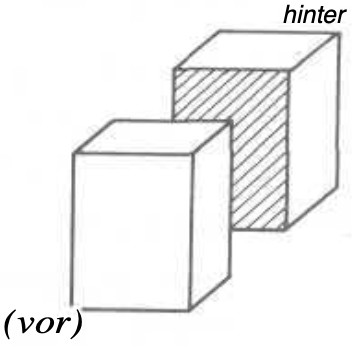
\includegraphics[scale=0.3]{hinter1.png}
            \end{figure}
        \end{itemize}
        \item (A) Zielgerichtet
        \begin{itemize}
            \item Sie haben die Garage hinter das Haus gebaut
            \item Er stellte sich in der Schlange hinter mich
            \begin{figure}[H]
                \centering
                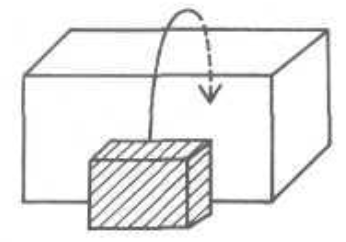
\includegraphics[scale=0.3]{hinter2.png}
            \end{figure}
        \end{itemize}
    \end{enumerate}
    \item (D nicht zielgerichtet, A zielgerichtet)比喻义
    \begin{itemize}
        \item Er wußte, daß seine Freunde hinter ihm stehen würden. (= helfen)
        \item Er wußte, daß seine Freunde sich hinter ihn stellen würden
    \end{itemize}
\end{enumerate}

\subsection{in(D/A)}
\begin{enumerate}
    \item Lokal
    \begin{enumerate}
        \item (D)Nicht zielgerichtet
        \begin{itemize}
            \item Das Buch liegt im Schrank
            \item Die Kinder sind in der Schule
            \begin{figure}[H]
                \centering
                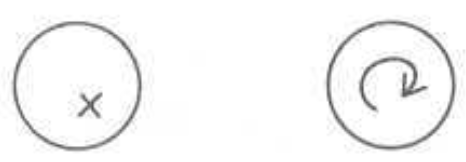
\includegraphics[scale=0.3]{in.png}
            \end{figure}
        \end{itemize}
        \item(A) Zielgerichtet
        \begin{itemize}
            \item Sie legt das Buch in den Schrank
            \item Die Kinder gehen in die Schule
            \begin{figure}[H]
                \centering
                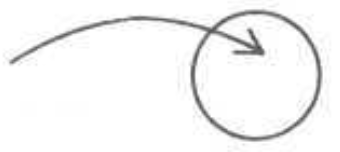
\includegraphics[scale=0.3]{in2.png}
            \end{figure}
        \end{itemize}
    \end{enumerate}
    \item (D)Temporal
    \begin{enumerate}
        \item Gleichzeitigkeit. Begrenzte Zeitdauer(= binnen, innerhalb)
        \begin{itemize}
            \item Wir hatten die Arbeit in zwei Tagen geschafft
        \end{itemize}
        \item Zeitpunkt nach der Sprechergegenwart
        \begin{itemize}
            \item In einem Jahr wird der Vertrag abgeschlossen sein
            \item Morgen in vierzehn Tagen bekommen wir Besuch. ( = 14 Tage nach morgen)
        \end{itemize}
        \item Gleichzeitigkeit. Zeitpunkt, Zeitdauer
        \begin{itemize}
            \item Sie ist im Jahre 1940 geboren
            \item Im Frühling fahren wir nach Berlin
            \item Erst in der letzten Sekunde besiegte er seinen Gegner
        \end{itemize}
    \end{enumerate}
    \item Modal
    \begin{enumerate}
        \item (D)Begleitender Umstand(=mit)
        \begin{itemize}
            \item Sie kamen in der Absicht, ihr zu helfen
        \end{itemize}
        \item(无格)用于语言名称前(=auf)
        \begin{itemize}
            \item Er hält seine Vorlesungen in russisch
        \end{itemize}
        \item(无格)用于颜色名称前
        \begin{itemize}
            \item Haben Sie dieses Kleid auch in grün
        \end{itemize}
        \item Zustand oder Zustandsveränderung;固定搭配中无冠词
        \begin{enumerate}
            \item(D)Zustand
            \begin{itemize}
                \item Die Maschine war in Betrieb.
            \end{itemize}
            \item(A)Zustandsveränderung
            \begin{itemize}
                \item Als die Maschine repariert war, konnte sie wieder in Gang gesetzt werden
            \end{itemize}
        \end{enumerate}
    \end{enumerate}
    \item 比喻义
    \begin{enumerate}
        \item(A/D)Bereich
        \begin{itemize}
            \item Er brachte dieses Problem in die Diskussion
        \end{itemize}
        \item Zustand oder Zustandsveränderung;用于Verbalsubstantiven前
        \begin{enumerate}
            \item (D)Zustand
            \begin{itemize}
                \item Wir waren im Diskutieren
                \item Die Arbeit ist im Werden
            \end{itemize}
            \item (A)Zustandsveränderung
            \begin{itemize}
                \item Wir kamen ins Diskutieren
            \end{itemize}
        \end{enumerate}
    \end{enumerate}
\end{enumerate}

\subsection{infolge(G)}
Kausal. Voraussetzung
\begin{itemize}
    \item Infolge eines Unfalls konnte er nicht mehr in seinem Betrieb arbeiten
    \item Infolge Nebels konnte das Flugzeug nicht starten
\end{itemize}

\subsection{inmitten(G)}
Lokal. Zentral in einem Bereich(=in)
\begin{itemize}
    \item Inmitten des Sees liegt eine Insel
    \item Der Werkleiter saß inmitten seiner Kollegen
    \begin{figure}[H]
        \centering
        
\includegraphics[scale=0.3]{inneri.png}
    \end{figure}
\end{itemize}

\subsection{innerhalb(G)}
\begin{enumerate}
    \item Lokal. Zu einem Bereich gehörig(=in)
    \begin{itemize}
        \item Innerhalb des Stadtgebietes ist die Fahrgeschwindigkeit begrenzt
        \item Innerhalb des Gebäudes darf nicht geraucht werden
        \begin{figure}[H]
            \centering
            
\includegraphics[scale=0.3]{innern.png}
        \end{figure}
    \end{itemize}
    \item Temporal. Gleichzeitigkeit. Begrenzte Zeitdauer(=während)
    \begin{itemize}
        \item Innerhalb eines Monats sollen wir die Arbeit abschließen
        \item Ich erwarte die Antwort auf meinen Brief innerhalb acht Tagen
    \end{itemize}
    \item 比喻义(=in)
    \begin{itemize}
        \item Das Gespräch bewegte sich immer innerhalb gewisser Grenzen
    \end{itemize}
\end{enumerate}

\subsection{je(A/N)}
Distributiv
\begin{enumerate}
    \item (A/N)常无冠词;也可无格(=pro)
    \begin{itemize}
        \item Ich habe 50 Pfennig je Kilo gezahlt
        \item Der Fahrpreis beträgt zwanzig Pfennig je angefangenen (angefangener) Kilometer
    \end{itemize}
    \item 双介词词置于je前/后
    \begin{itemize}
        \item Die Tabletten sind zu je sechs Stück verpackt
        \item Am Gemüsestand wird frisches Obst je nach der Jahreszeit verkauft
    \end{itemize}
\end{enumerate}

\subsection{je nach(D)}
根据……不同;因……而异

\subsection{jenseits(G)}
\begin{enumerate}
    \item Lokal
    \begin{itemize}
        \item Jenseits des Flusses liegt ein ausgedehnter Wald
        \item Der Berg mit dem Aussichtsturm befindet sich jenseits der Grenze
    \end{itemize}
    \item 比喻义(=außerhalb)
    \begin{itemize}
        \item Diese Problematik liegt jenseits seines Interesses
    \end{itemize}
\end{enumerate}


\subsection{Kraft(G)}
Modal. Instrumental. Amtssprache. Nur bei Abstrakta
\begin{itemize}
    \item Kraft seines Amtes ist er zu Änderungen an den Bauentwürfen be- rechtigt
\end{itemize}

\subsection{längs(G)}
Lokal. Parallelverlauf. (= entlang )
\begin{itemize}
    \item Sie wanderten längs des Flusses
    \item Längs der Straße standen Apfelbäume
    \item Er besitzt ein Stück Land längs des Bahndamms
\end{itemize}

\subsection{laut(G)}
Modal 按照、根据、相符;常无冠词
\begin{itemize}
    \item Laut dieses Berichts (diesem Bericht) hat der Betrieb einen hohen Gewinn erzielt
    \item Laut Gesetz ist der Alkoholausschank an Jugendliche verboten
\end{itemize}

\subsection{mit(D)}
\begin{enumerate}
    \item Modal
    \begin{enumerate}
        \item Instrumental(=mittels)
        \begin{itemize}
            \item Sie schreibt den Brief mit der Schreibmaschine
            \item Er ist mit dem Abendzug gekommen
            \item Mit wenigen W orten hat er die Situation charakterisiert
        \end{itemize}
        \item Begleitender Umstand;名词前有修饰词(obl./fak.)
        \begin{itemize}
            \item 名词属于客观情况,其前有修饰词(obl.)
            \begin{itemize}
                \item Mit hoher Geschwindigkeit fuhr der Zug über die Brücke
                \item Mit großen Schritten eilte er nach Hause
            \end{itemize}
            \item 名词属于主观情况,其前有修饰词(fak.)
            \begin{itemize}
                \item Mit (großem) Interesse verfolgten sie das Spiel.
            \end{itemize}
        \end{itemize}
    \end{enumerate}
    \item Temporal. Gleichzeitigkeit, Zeitpunkt(=bei)
    \begin{itemize}
        \item In vielen Ländern kommen die Kinder mit sechs Jahren in die Schule
        \item Mit dem Startschuß setzten sich die Läufer in Bewegung
    \end{itemize}
    \item Konditional
    \begin{itemize}
        \item Mit etwas Glück kann er die Prüfung schaffen.
    \end{itemize}
    \item Partitiv. Zugehörigkeit. Teil-von-Verhältnis
    \begin{itemize}
        \item Ein Tisch mit drei Beinen
        \item Ein Zimmer mit Frühstück
    \end{itemize}
\end{enumerate}


\subsection{mittels(G)}
Modal. Instrumental. Vor allem in technischen Fachsprachen;Dativ当Gentiv无法识别
\begin{itemize}
    \item Die Tür mußte mittels eines Schweißgeräts geöffnet werden
    \item Die Raumfahrer schützen sich mittels Spezialanzügen gegen kosmi- sche Strahlen
\end{itemize}


\subsection{nach(D)}
\begin{enumerate}
    \item Lokal. Zielgerichtet. 在空间副词和地名前;大部分无冠词
    \begin{itemize}
        \item Gehen Sie bitte nach rechts
        \item Die Vögel fliegen nach Süden
    \end{itemize}
    \begin{enumerate}
        \item 有冠词时多用in
        \begin{itemize}
            \item Die Studentengruppe fährt in die Schweiz
            \item Die Vögel fliegen im Herbst in den Süden
        \end{itemize}
    \end{enumerate}
    \item Temporal. Vorzeitigkeit. Mit Angabe des Ausgangspunktes
    \begin{itemize}
        \item Wir sind erst nach Mitternacht in Leipzig angekommen
        \item Nach dem Essen geht sie immer spazieren
    \end{itemize}
    \item Modal
    \begin{enumerate}
        \item 程度;与最高级连用
        \begin{itemize}
            \item Nach Hans ist Werner der Größte in der Klasse
            \item Nach dem Schwimmen gefällt mir der Langlauf am besten
        \end{itemize}
        \item 等级、顺序;Prä- und Poststellung
        \begin{itemize}
            \item Sie standen der Größe nach (nach der Größe) nebeneinander
            \item Die Waren wurden nach der Qualität (der Qualität nach) sortiert
        \end{itemize}
        \item 按照、根据;Prä- und Poststellung
        \begin{itemize}
            \item Allem Anschein nach (nach allem Anschein) wird es heute noch regnen
            \item Nach den Hygienevorschriften (den Hygienevorschriften nach) müßte das Geschäft geschlossen werden
            \item Nach Herder ist die Humanität das Ziel des geschichtlichen Fort- schritts.
        \end{itemize}
    \end{enumerate}
    \item nach und nach(=allmählich)逐渐地
    \begin{itemize}
        \item Nach und nach versammelten sich die Gäste
    \end{itemize}
    \item nach wie vor(=noch immer)仍然
    \begin{itemize}
        \item Nach wie vor macht er beim Sprechen viele Fehler
    \end{itemize}
\end{enumerate}

\subsection{neben(D/A)}
\begin{enumerate}
    \item Lokal
    \begin{enumerate}
        \item(D)Nicht zielgerichtet
        \begin{itemize}
            \item Die Lampe steht neben dem Schrank
            \item Sie geht neben ihm
            \begin{figure}[H]
                \centering
                
\includegraphics[scale=0.3]{neben1.png}
            \end{figure}
        \end{itemize}
        \item(A)Zielgerichtet
        \begin{itemize}
            \item Sie stellt die Lampe neben den Schrank
            \item Sie setzt sich neben ihn
            \begin{figure}[H]
                \centering
                
\includegraphics[scale=0.3]{neben2.png}
            \end{figure}
        \end{itemize}
    \end{enumerate}
    \item(D)Kopulativ(=außer)
    \begin{itemize}
        \item Neben seiner beruflichen Arbeit hat er noch eine Menge Hobbys
        \item Neben einigen afrikanischen Studenten nahmen auch Südamerika- ner an der Exkursion teil
    \end{itemize}
\end{enumerate}

\subsection{ob(G)}
(=wegen)
\begin{itemize}
    \item Ob des schlechten Wetters blieben wir zu Hause
\end{itemize}
\subsection{oberhalb(G)}
Lokal. Höhere Lage(=über)
\begin{itemize}
    \item Er stand oberhalb des Hanges.
    \item Oberhalb des ersten Stockwerks brach
    \begin{figure}[H]
        \centering
        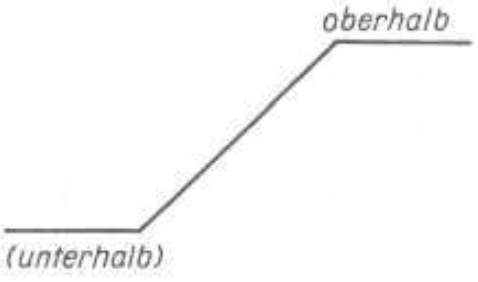
\includegraphics[scale=0.3]{ober.png}
    \end{figure}
\end{itemize}

\subsection{ohne(A)}
\begin{enumerate}
    \item Modal
    \begin{enumerate}
        \item Instrumental. Negation
        \begin{itemize}
            \item Ohne ein Spezialwerkzeug kann die Tür nicht geöffnet werden
        \end{itemize}
        \item Begleitender Umstand. Negation
        \begin{itemize}
            \item Er las das Buch ohne großes Interesse
            \item Das Zimmer ist ohne Frühstück berechnet
        \end{itemize}
        \item Konditional. Negation
        \begin{itemize}
            \item Ohne Zufuhr von Düngemitteln läßt der Boden bald in seiner Fruchtbarkeit nach
        \end{itemize}
        \item Restriktiv. 与数词连用(=außer)
        \begin{itemize}
            \item Ohne die Kinder waren es zehn Gäste
            \item Ohne den Lehrer waren dreißig Personen im Raum
        \end{itemize}
    \end{enumerate}
\end{enumerate}

\subsection{per(A)}
durch 3
\subsection{pro(A)}
je 1


\subsection{(mit)samt(D)}
Modal. Begleitender Umstand. 可无冠词
\begin{itemize}
    \item Der Lastwagen ist (mit)samt (dem) Anhänger umgekippt.
\end{itemize}


\subsection{seit(D)}
\begin{enumerate}
    \item Temporal. Zeitdauer bis Sprechergegenwart mit Anfangspunkt in der Vergangenheit
    \begin{itemize}
        \item Seit drei Monaten liegt seine Frau im Krankenhaus
        \item Sie haben sich seit acht Jahren nicht gesehen
    \end{itemize}
    \item 
\end{enumerate}

\subsection{seiten(s)(G)}
Urheber(=von, durch)

\begin{itemize}
    \item Seitens der Stadtverwaltung wird das Bauvorhaben unterstützt
    \item Seitens des Arztes gibt es keine Einwände, daß er Sport treibt
\end{itemize}

\subsection{(an)statt(G)}
Ersatz, Austausch(= an Stelle von, für);口语中也用Dativ
\begin{itemize}
    \item Statt eines Fernsehapparates kauften sie ein Radio
    \item (An)statt Blumen habe ich Ihnen ein Buch mitgebracht
\end{itemize}



\subsection{trotz(G)}
Konzessiv(=ohne Rücksicht auf);少数情况用Dativ
\begin{itemize}
    \item Trotz des schlechten Wetters gingen wir spazieren
    \item Trotz dem Verbot des Vaters ging der Junge auf das Eis
\end{itemize}

\subsection{über}
\begin{enumerate}
    \item Lokal
    \begin{enumerate}
        \item (D)Nichtzielgerichtet
        \begin{itemize}
            \item Das Bild hängt über dem Schreibtisch
            \item Das Flugzeug kreist über der Stadt
            \begin{figure}[H]
                \centering
                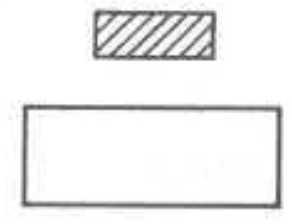
\includegraphics[scale=0.3]{uber1.png}
            \end{figure}
        \end{itemize}
        \item (A)zielgerichtet
        \begin{itemize}
            \item Sie hängt das Bild über den Schreibtisch
            \item Der Wagen ist über den Sperrstreifen gefahren
            \begin{figure}[H]
                \centering
                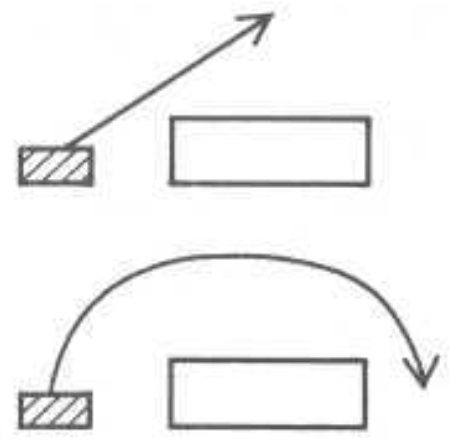
\includegraphics[scale=0.3]{uber2.png}
            \end{figure}
        \end{itemize}
        \item(A)Geographisch 车站、航线
        \begin{itemize}
            \item Fährt die Straßenbahn über den Bahnhof?
            \item Die Maschine fliegt über Prag nach Sofia
        \end{itemize}
    \end{enumerate}
    \item(无格)Modal. Steigende Wiederholung
    \begin{itemize}
        \item In seinem Aufsatz sind Fehler über Fehler
        \item Fragen über Fragen wurden gestellt
    \end{itemize}
    \item(A)Temporal. Gleichzeitigkeit. Begrenzte Zeitdauer;Poststellung;Fak. Gebrauch(=hindurch)
    \begin{itemize}
        \item Die letzten drei Jahre (über) waren die Sommer kühl
        \item Die Nacht (über) hat es geregnet
    \end{itemize}
\end{enumerate}

\subsection{um(A)}
\begin{enumerate}
    \item Lokal. Verhältnis zu einem Mittelpunkt
    \begin{itemize}
        \item Das Auto fährt um die Eck
        \item Der Junge läuft um einen Baum
        \item Die Studenten sind um den Dozenten versammelt
        \begin{figure}[H]
            \centering
            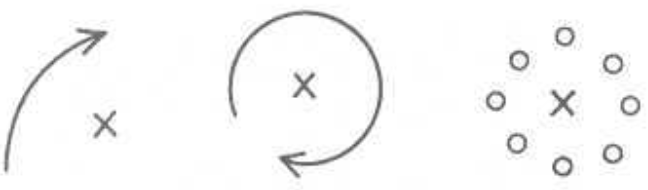
\includegraphics[scale=0.3]{um.png}
        \end{figure}
    \end{itemize}
    \item Temporal. 确定或不确定
    \begin{enumerate}
        \item 不确定时间(= ungefähr, etwa, gegen)
        \begin{itemize}
            \item Dieses Haus ist um 1900 erbaut
            \item Die Prüfung findet um den 20. Januar statt
        \end{itemize}
        \item 确定的小时
        \begin{itemize}
            \item Kommen Sie bitte um 19 Uhr zu mir
        \end{itemize}
        \begin{enumerate}
            \item 小时词作为谓语时=常无介词,有介词的情况常出现于口语中
        \end{enumerate}
    \end{enumerate}
    \item (无格)Modal. Steigernde Wiederholung
    \begin{itemize}
        \item Tag um Tag wartet er auf Antwort
        \item Ich habe Seite um Seite gelesen, die Stelle aber nicht gefunden
    \end{itemize}
\end{enumerate}

\subsection{um……willen(G)}
Kausal. Grund(=wegen)
\begin{itemize}
    \item Um seiner Gesundheit willen hat er das Rauchen aufgegeben
    \item Um der Kinder willen ließen sie sich nicht scheiden
\end{itemize}

\subsection{ungeachtet(G)}
Konzessiv. Vor Abstrakta. Prä- und Poststellung;文学语言中用Poststellung
\begin{itemize}
    \item Ungeachtet verschiedener Schwierigkeiten hat sie ihre Arbeit termingemäß abgeschlossen
    \item Seiner schlechten Kondition ungeachtet nahm er am Wettkampf teil. Ungeachtet wiederholter Beschwerden der Hausbewohner wurde der Müll nicht pünktlich abgefahren
\end{itemize}

\subsection{unter(D/A)}
\begin{enumerate}
    \item Lokal
    \begin{enumerate}
        \item (D)Nichtzielgerichtet
        \begin{itemize}
            \item Unter dem Tisch liegt ein Teppich
            \begin{figure}[H]
                \centering
                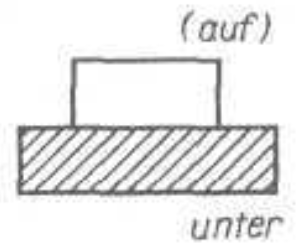
\includegraphics[scale=0.3]{unter1.png}
            \end{figure}
        \end{itemize}
        \item (A)zielgerichtet
        \begin{itemize}
            \item Sie nimmt die Tasche unter den Arm.
            \begin{figure}[H]
                \centering
                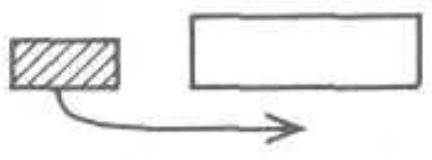
\includegraphics[scale=0.3]{unter2.png}
            \end{figure}
        \end{itemize}
        \item 位于人群或物品之间的位置
        \begin{enumerate}
            \item (D)Nichtzielgerichtet
            \begin{itemize}
                \item Er hat bisher immer nur unter Gleichaltrigen gelebt
                \item Unter den Steinen befand sich ein Diamant
                \begin{figure}[H]
                    \centering
                    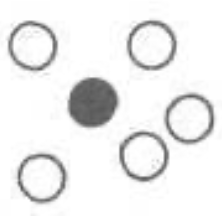
\includegraphics[scale=0.3]{unter3.png}
                \end{figure}
            \end{itemize}
            \item (A)zielgerichtet
            \begin{itemize}
                \item Er kam unter Gleichaltrige
                \item Ich mischte mich unter die Zuschauer
                \begin{figure}[H]
                    \centering
                    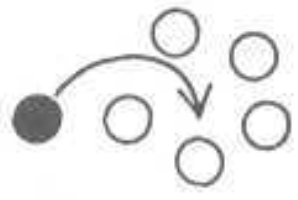
\includegraphics[scale=0.3]{unter4.png}
                \end{figure}
            \end{itemize}
        \end{enumerate}
    \end{enumerate}
    \item (D)Modal
    \begin{enumerate}
        \item Begleitender Umstand(=mit)
        \begin{itemize}
            \item Unter großem Beifall wurde der Redner vorgestellt
            \item Unter Jubel und Gelächter fiel der Vorhang
        \end{itemize}
        \item 固定搭配,表示条件
        \begin{itemize}
            \item Er kann die Prüfung nur unter der Voraussetzung bestehen, daß man ihm bei der Vorbereitung hilft
        \end{itemize}
    \end{enumerate}
    \item 比喻义
    \begin{itemize}
        \item Der Roman handelt von den Verhältnissen unter Ludwig XIV
        \item Die Tagung findet unter der Leitung des Ministers statt
    \end{itemize}
\end{enumerate}

\subsection{unterhalb(G)}
Lokal
\begin{itemize}
    \item Das Feuer war unterhalb der zweiten Etage ausgebrochen
\end{itemize}

\subsection{unweit, unfern(G)}
Lokal 附近
\begin{itemize}
    \item Unweit der Eisenbahnlinie entsteht eine neue Stadt
\end{itemize}

\subsection{von(D)}
\begin{enumerate}
    \item Lokal
    \begin{enumerate}
        \item 一般的出发点
        \begin{itemize}
            \item Er sprang von der Straßenbahn
        \end{itemize}
        \item 具体的出发点;双介词在被修饰词后(Circumstellung)
        \begin{itemize}
            \item Von der Brücke an fuhr das Auto langsam
            \item Vom Flugzeug aus war die Gegend gut zu überblicken.
        \end{itemize}
        \item 一段距离的出发点;双介词分别在起点和终点前
        \begin{itemize}
            \item Der Bus fährt von Leipzig bis Dresden
            \item Wir fliegen von Berlin nach Moskau
        \end{itemize}
    \end{enumerate}
    \item Temporal. Zeitdauer mit Angabe des Anfangspunktes
    \begin{enumerate}
        \item 双介词/her在被修饰词后
        \begin{itemize}
            \item Von acht Uhr ab bin ich wieder zu Hause
            \item Er spielt von Jugend auf Klavier
            \item Wir feiern von alters her Silvester zu Hause
        \end{itemize}
        \item bis在第二个被修饰词前
        \begin{itemize}
            \item Von zehn Uhr bis zehn Uhr dreißig ist Pause
        \end{itemize}
    \end{enumerate}
    \item Modal
    \begin{enumerate}
        \item Qualität. Eigenschaft
        \begin{itemize}
            \item Sie war eine Frau von großer Schönheit
            \item Wir sahen ein Theaterstück von hohem Niveau
        \end{itemize}
        \item Qualität. Stoffliche Beschaffenheit(=aus)
        \begin{itemize}
            \item Sie kaufte einen Ring von (purem) Gold
            \item Der Ring ist von (purem) Gold
        \end{itemize}
        \item Urheber, Agens(=durch)
        \begin{itemize}
            \item Das Kind wurde von seinen Eltern nie geschlagen
            \item Dresden wurde von Flugzeugen zerstört.
        \end{itemize}
        \item Partitiv. Teil-von-Verhältnis. Auswahl
        \begin{itemize}
            \item Von allen Studenten war er der fleißigste
        \end{itemize}
    \end{enumerate}
\end{enumerate}

\subsection{vor(D/A)}
\begin{enumerate}
    \item Lokal
    \begin{enumerate}
        \item (D)Nichtzielgerichtet
        \begin{itemize}
            \item Das Taxi steht vor dem Hoteleingang
            \item Bei der Demonstration marschierte er vor mir.
        \end{itemize}
        \item (A)zielgerichtet
        \begin{itemize}
            \item Das Taxi fährt vor den Hoteleingan
            \item Bei der Demonstration stellte er sich vor mich
        \end{itemize}
    \end{enumerate}
    \item (D)Temporal
    \begin{enumerate}
        \item Zeitpunkt vor der Sprechergegenwart.
        \begin{itemize}
            \item Vor einer Woche haben die Ferien begonnen
            \item Gestern vor vierzehn Tagen ist er abgefahren
        \end{itemize}
        \item Nachzeitigkeit. Mit Angabe des Endpunktes
        \begin{itemize}
            \item Vor 1945 war Mecklenburg vorwiegend Agrarland
            \item Vor dem Schlafengehen soll der Patient Spazierengehen
        \end{itemize}
        \item Zeitpunkt nach der Sprechergegenwart
        \begin{itemize}
            \item Vor Ende dieses Monats wird die Arbeit nicht beendet sein
            \item Wir erwarten ihn nicht vor heute abend
        \end{itemize}
    \end{enumerate}
    \item(D)Kasul 无冠词
    \begin{itemize}
        \item Die Kinder schrien vor Begeisterung
        \item Vor Nebel war nichts zu sehen
        \item Vor Lärm konnte man nichts hören
    \end{itemize}
\end{enumerate}

\subsection{während(G)}
Temporal. Gleichzeitigkeit. Zeitdauer(=auf, bei);Genitiv无法识别时用Dativ,口语中也用Dativ
\begin{itemize}
    \item Während der Sommerferien arbeiten viele Studenten in den Betrieben
    \item Während der Arbeit darf auf der Baustelle weder geraucht noch ge- trunken werden
\end{itemize}

\subsection{wegen(G)}
Kausal. Grund;Auch in Poststellung;口语中也用Dativ
\begin{itemize}
    \item Die Vorlesung fiel wegen (der) Erkrankung des Professors aus
    \item Des starken Frostes wegen heizen wir jetzt zweimal am Tag
\end{itemize}

\subsection{(zu)wider(A)}
\begin{enumerate}
    \item wider; Adversativ. Vor Abstrakta
    \begin{itemize}
        \item Die beiden haben wider das Gesetz gehandelt
        \item Wider Willen mußte sie lachen
    \end{itemize}
    \item zuwider, Poststellung
    \begin{itemize}
        \item Otto handelt der Abmachung zuwider
    \end{itemize}
\end{enumerate}

\subsection{wie(无格)}
Modal. Komparativ. Gleichheit im Vergleich
\begin{itemize}
    \item Sie liebte ihn wie einen Vater.
    \item Der Ausländer spricht Deutsch wie ein Muttersprachler
\end{itemize}


\subsection{zu(D)}
\begin{enumerate}
    \item Lokal. Zielgerichtet
    \begin{itemize}
        \item Wir gehen zum Bahnhof
    \end{itemize}
    \begin{enumerate}
        \item 在地名前用nach不用zu
    \end{enumerate}
    \item Temporal. Gleichzeitigkeit. Zeitpunkt, Zeitdauer
    \begin{itemize}
        \item Kommt ihr heute zum Abendessen
        \item Er hat uns zum Jahresende besucht
        \item Diese Arbeit muß (bis) zum 1. September fertig sein
        \item Zur Hochzeit erhielten sie viele Geschenke.
    \end{itemize}
    \item Final. Vor Deverbativa.
    \begin{enumerate}
        \item Zumeist mit Artikelverschmelzung(=für)
        \begin{itemize}
            \item Zum Gelingen des Festes waren viele Vorbereitungen nötig
            \item Er ist zum Training auf den Sportplatz gegangen
        \end{itemize}
        \item Mit modal-spezifizierender Nebenbedeutung. Obl. Artikelverschmelzun(=als)
        \begin{itemize}
            \item Zum Andenken schenkte er ihr ein Armband
            \item Sie tranken eine Limonade zur Erfrischung
        \end{itemize}
    \end{enumerate}
    \item Distributiv
    \begin{enumerate}
        \item Personengruppe. V or endungslosen Ordinalia und vor Kardinalia mit Endung -en 
        \begin{itemize}
            \item Die Soldaten marschierten zu dritt in einer Reihe
            \item Die Soldaten marschierten zu dreien in einer Reihe
        \end{itemize}
        \item Relation zwischen zwei Zahlangaben
        \begin{itemize}
            \item Sie kaufte zwei Kilo Äpfel zu drei Mark
            \item Ich habe zwei Päckchen Kaffee zu hundert Gramm genommen.
        \end{itemize}
    \end{enumerate}
    \item Modal. Instrumental. Art der Fortbewegung. In festen Verbindun- gen. Bei Maskulina und Neutra mit Nullartikel
    \begin{itemize}
        \item Das Manöver wurde zu Wasser, zu Lande und in der Luft durchgeführt
    \end{itemize}
    \item Konsekutiv 承接、结果
    \begin{itemize}
        \item Die Zwillinge sind sich zum Verwechseln ähnlich
        \item Die Feier gestaltete sich zu einem großen Erlebnis
    \end{itemize}
\end{enumerate}


\subsection{zufolge(D)}
\begin{enumerate}
    \item Kausal. Zumeist in Poststellung
    \begin{itemize}
        \item Dem V ertrag zufolge (zufolge des V ertrages) werden große Mengen Weizen importiert
    \end{itemize}
    \item Modal. Entsprechung. Gewöhnlich in Poststellung
    \begin{itemize}
        \item Einer Pressemeldung zufolge ist der ausländische Gast eingetroffen
    \end{itemize}
\end{enumerate}

\subsection{zugunsten(G)}
Final. (= im Interesse von)
\begin{itemize}
    \item Sie ist zugunsten eines Kollegen (einem Kollegen zugunsten) von der Reise zurückgetreten.
    \item Er hat zugunsten des Roten Kreuzes auf das Honorar verzichtet
\end{itemize}

\subsection{zuzüglich(G)}
另加
\begin{itemize}
    \item Der Preis beträgt 100 Euro, zuzüglich Versandkosten
\end{itemize}
\subsection{zuliebe(D)}
Final-Kausal. In Poststellung

\begin{itemize}
    \item Seiner Frau zuliebe ist er zu Hause geblieben
\end{itemize}

\subsection{zwischen(D/A)}
\begin{enumerate}
    \item Lokal. Vor zwei mit und verbundenen Substantiven oder einem Substantiv im Plural
    \begin{enumerate}
        \item(D) Nichtzielgerichtet
        \begin{itemize}
            \item Zwischen dem Schrank und dem Bett steht ein Tisch
            \item Sie ging zwischen meinem Freund undmir
            \begin{figure}[H]
                \centering
                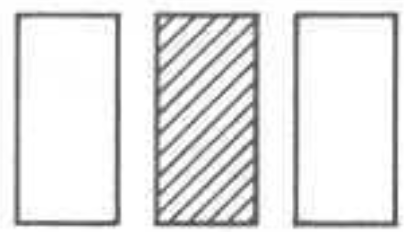
\includegraphics[scale=0.3]{zw1.png}
            \end{figure}
        \end{itemize}
        \item(A) zielgerichtet
        \begin{itemize}
            \item Sie haben den Tisch zwischen den Schrank und das Bett gestellt
            \item Er stellte sich zwischen meinen Freund und mich
            \begin{figure}[H]
                \centering
                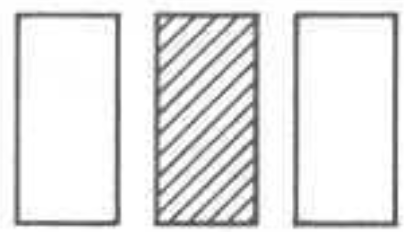
\includegraphics[scale=0.3]{zw1.png}
            \end{figure}
        \end{itemize}
    \end{enumerate}
    \item (无格)Modal/Temporal 不确定的时间/尺度;Vor zwei mit und verbundenen Zahlen, mit denen die Begren- zung angegeben wird. 无冠词
    \begin{itemize}
        \item Die Temperatur beträgt zwischen 8 und 12 Grad
        \item Der Dichter ist zwischen 1410 und 1420 geboren
    \end{itemize}
    \item(D nicht zielgerichtet, A zielgerichtet)从Lokal引申来的比喻义
    \begin{itemize}
        \item Der Handel zwischen den Vertragspartnern entwickelt sich immer intensiver
        \item Er hat versucht, einen Keil zwischen die Freunde zu treiben
    \end{itemize}
\end{enumerate}

\chapter{Junktion}


\section{Konjunktion}
\subsection{Additive}
\begin{figure}[H]
    \centering
    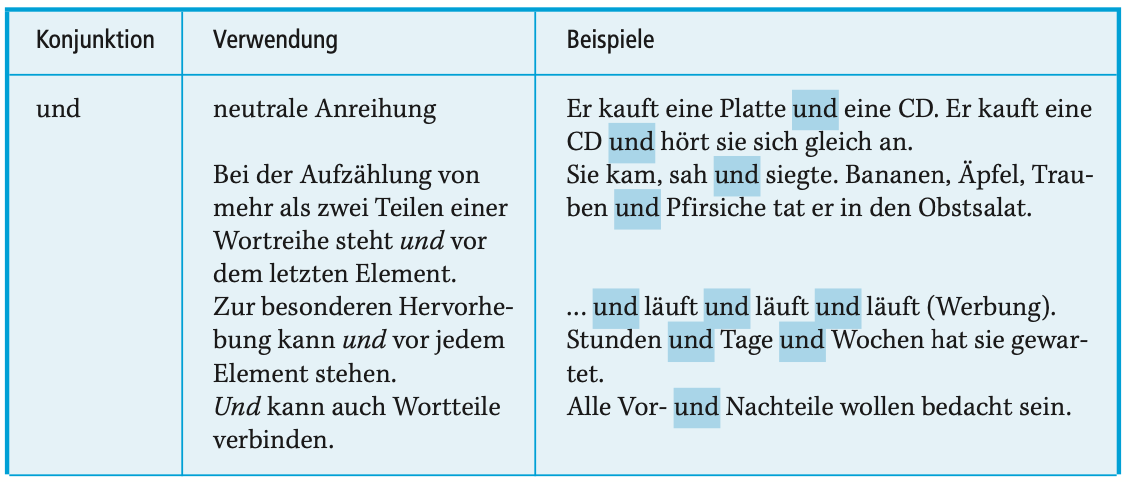
\includegraphics[scale=0.6]{add1.png}
\end{figure}
\begin{figure}[H]
    \centering
    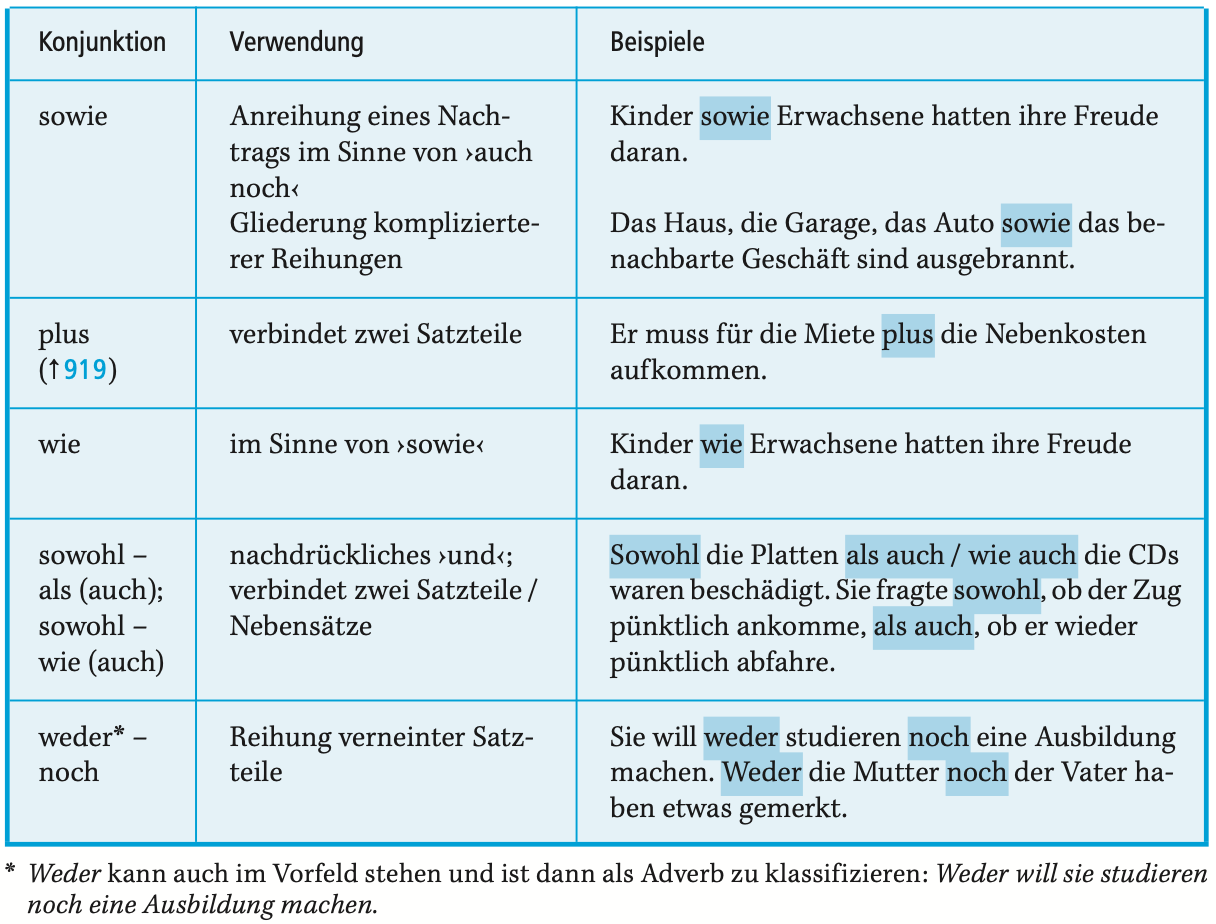
\includegraphics[scale=0.55]{add2.png}
\end{figure}


\subsection{Alternative}
\begin{figure}[H]
    \centering
    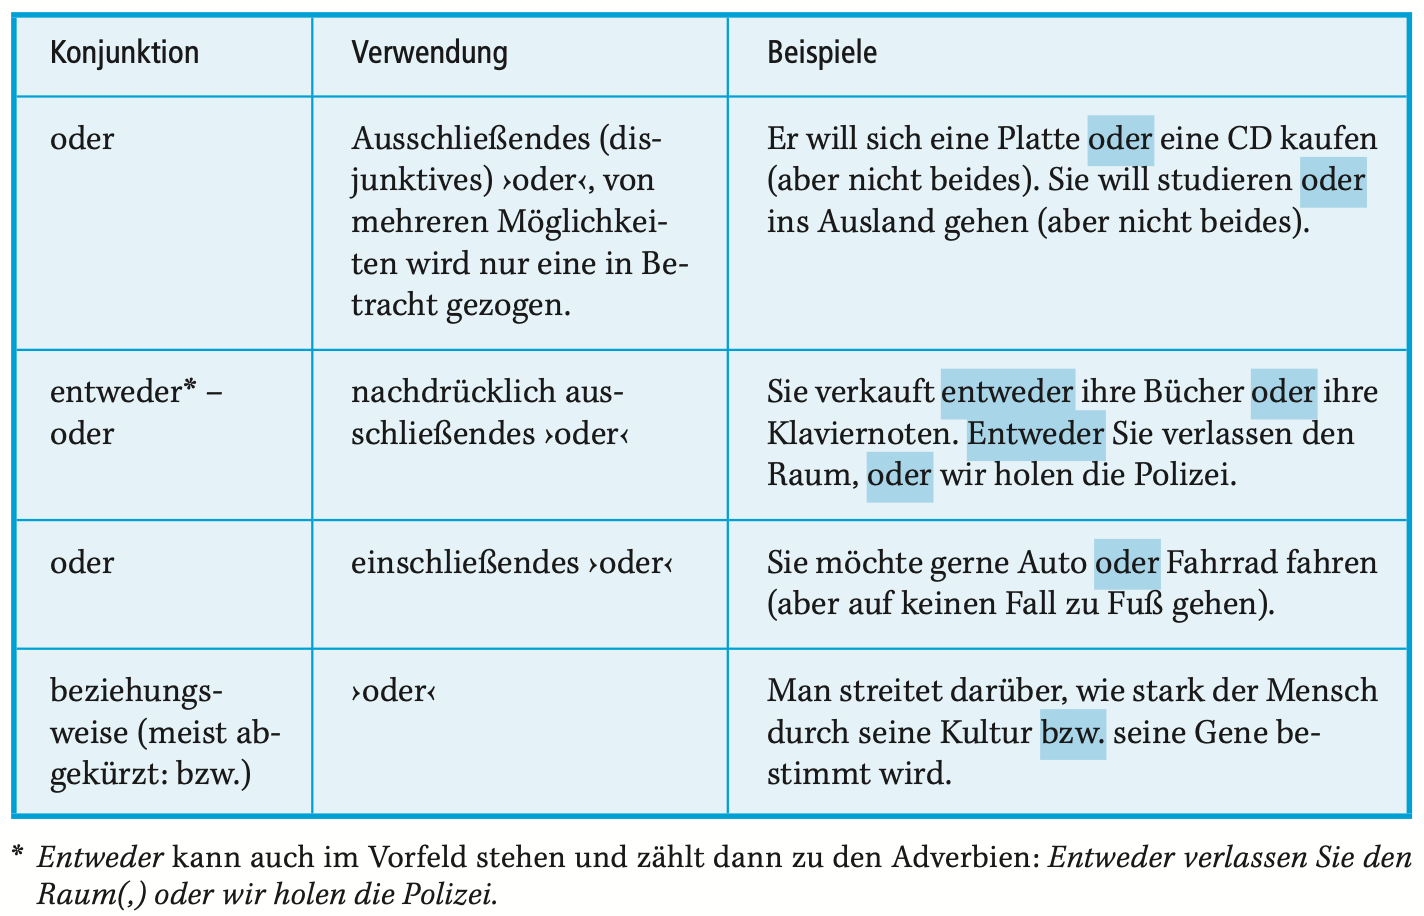
\includegraphics[scale=0.55]{alt.png}
\end{figure}

\subsection{Adversative/Konzessive}
\begin{figure}[H]
    \centering
    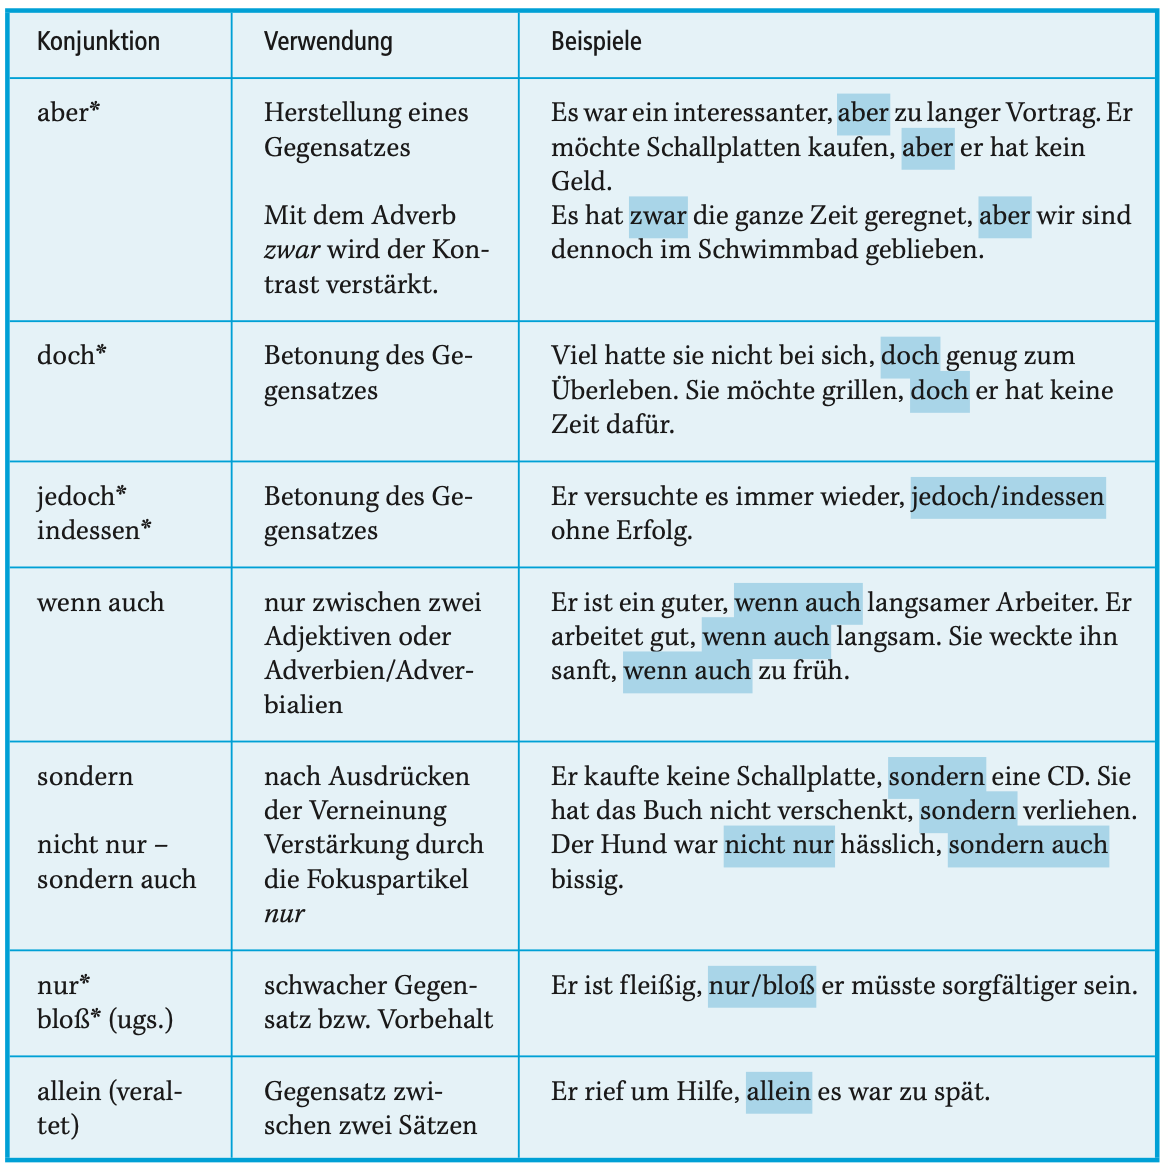
\includegraphics[scale=0.65]{knz.png}
\end{figure}

\subsection{Spezifizieren}
\begin{figure}[H]
    \centering
    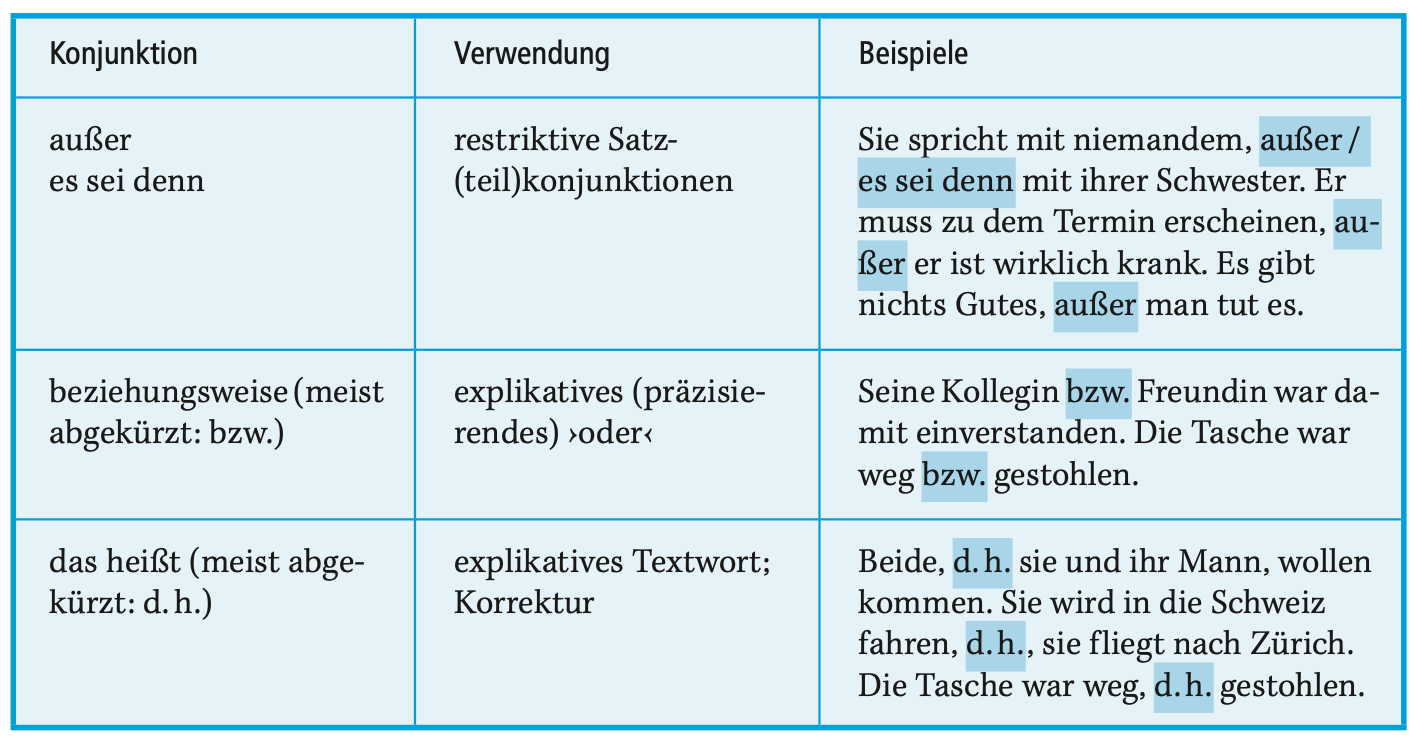
\includegraphics[scale=0.55]{spc.png}
\end{figure}

\subsection{Kasual}
\begin{figure}[H]
    \centering
    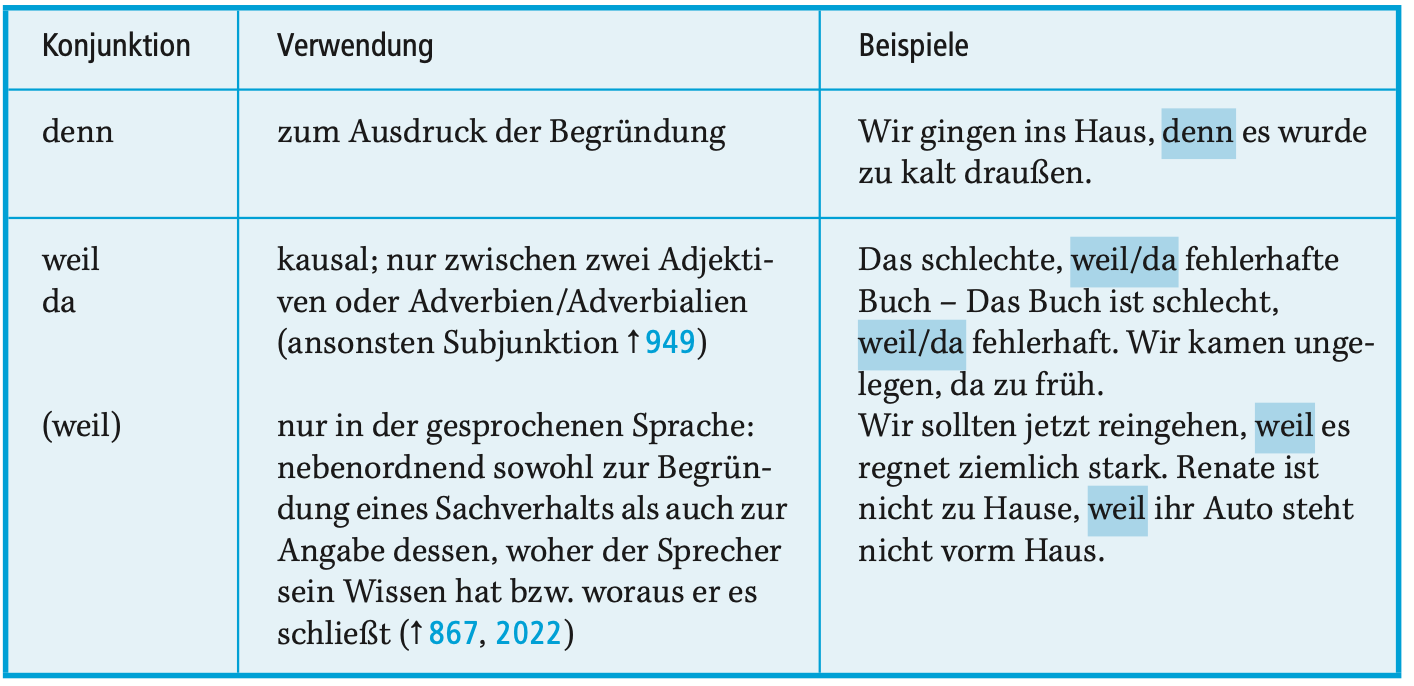
\includegraphics[scale=0.55]{kc.png}
\end{figure}

\subsection{Vergleich}
\begin{figure}[H]
    \centering
    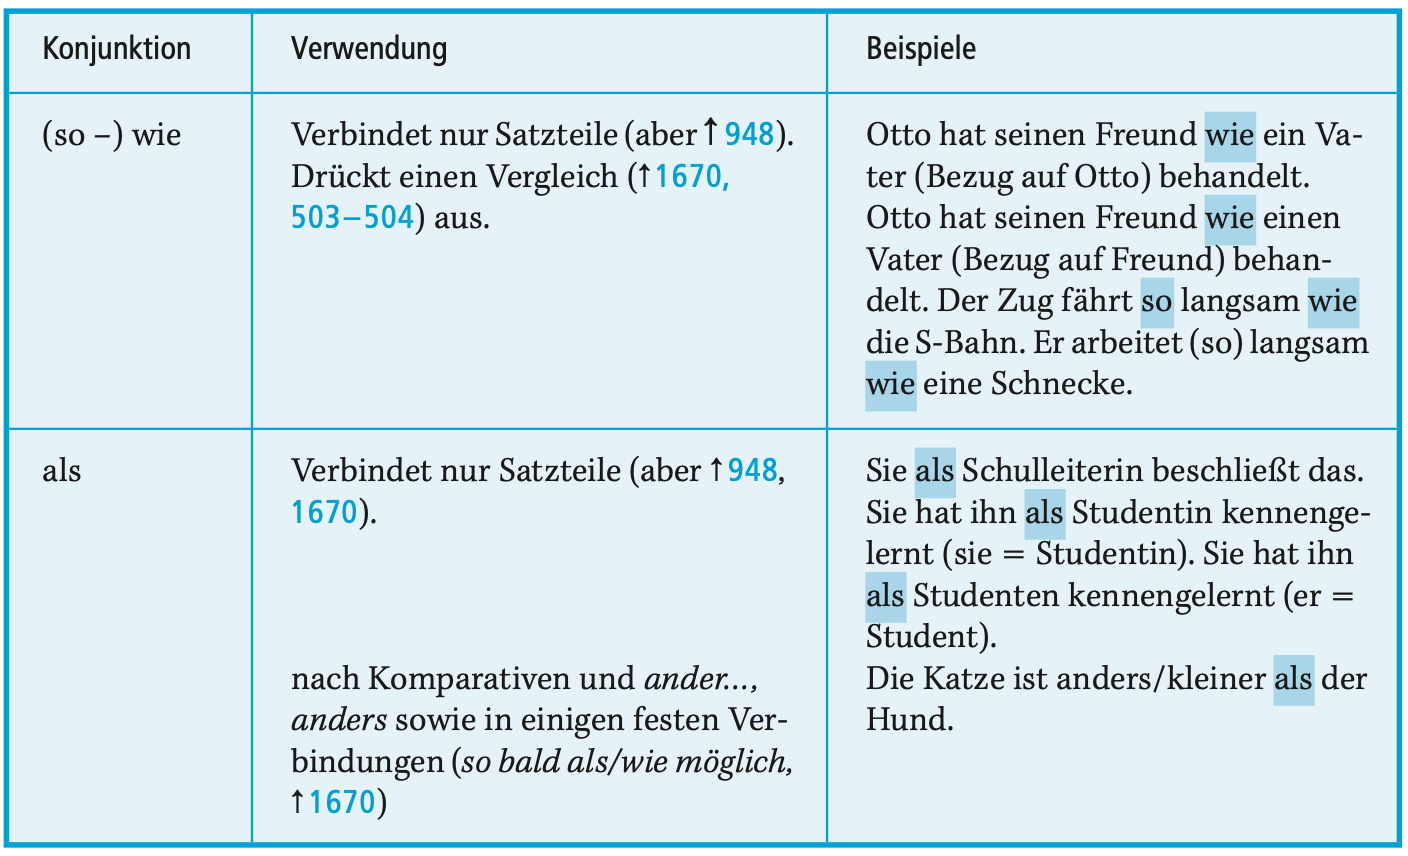
\includegraphics[scale=0.55]{ver.png}
\end{figure}



\section{Subjunktion}
Um, ohne, anstatt, außer单独时只与Infinitiv连用

\subsection{Neutral}
\begin{figure}[H]
    \centering
    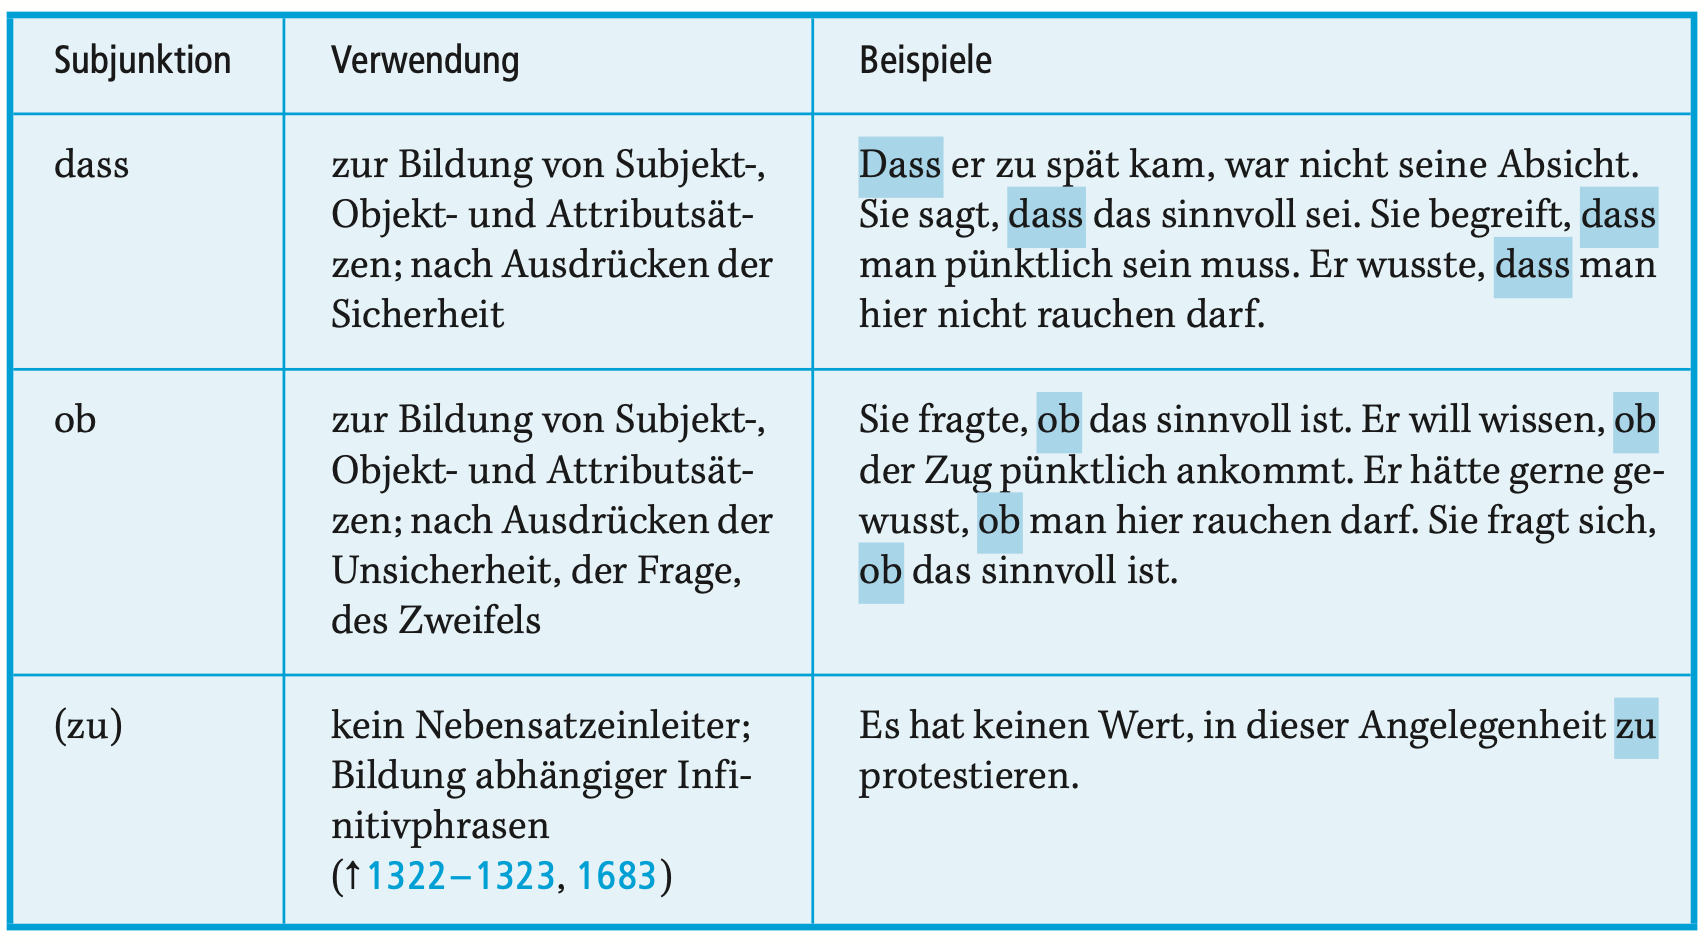
\includegraphics[scale=0.55]{nu.png}
\end{figure}

\subsection{Temporal}
\begin{figure}[H]
    \centering
    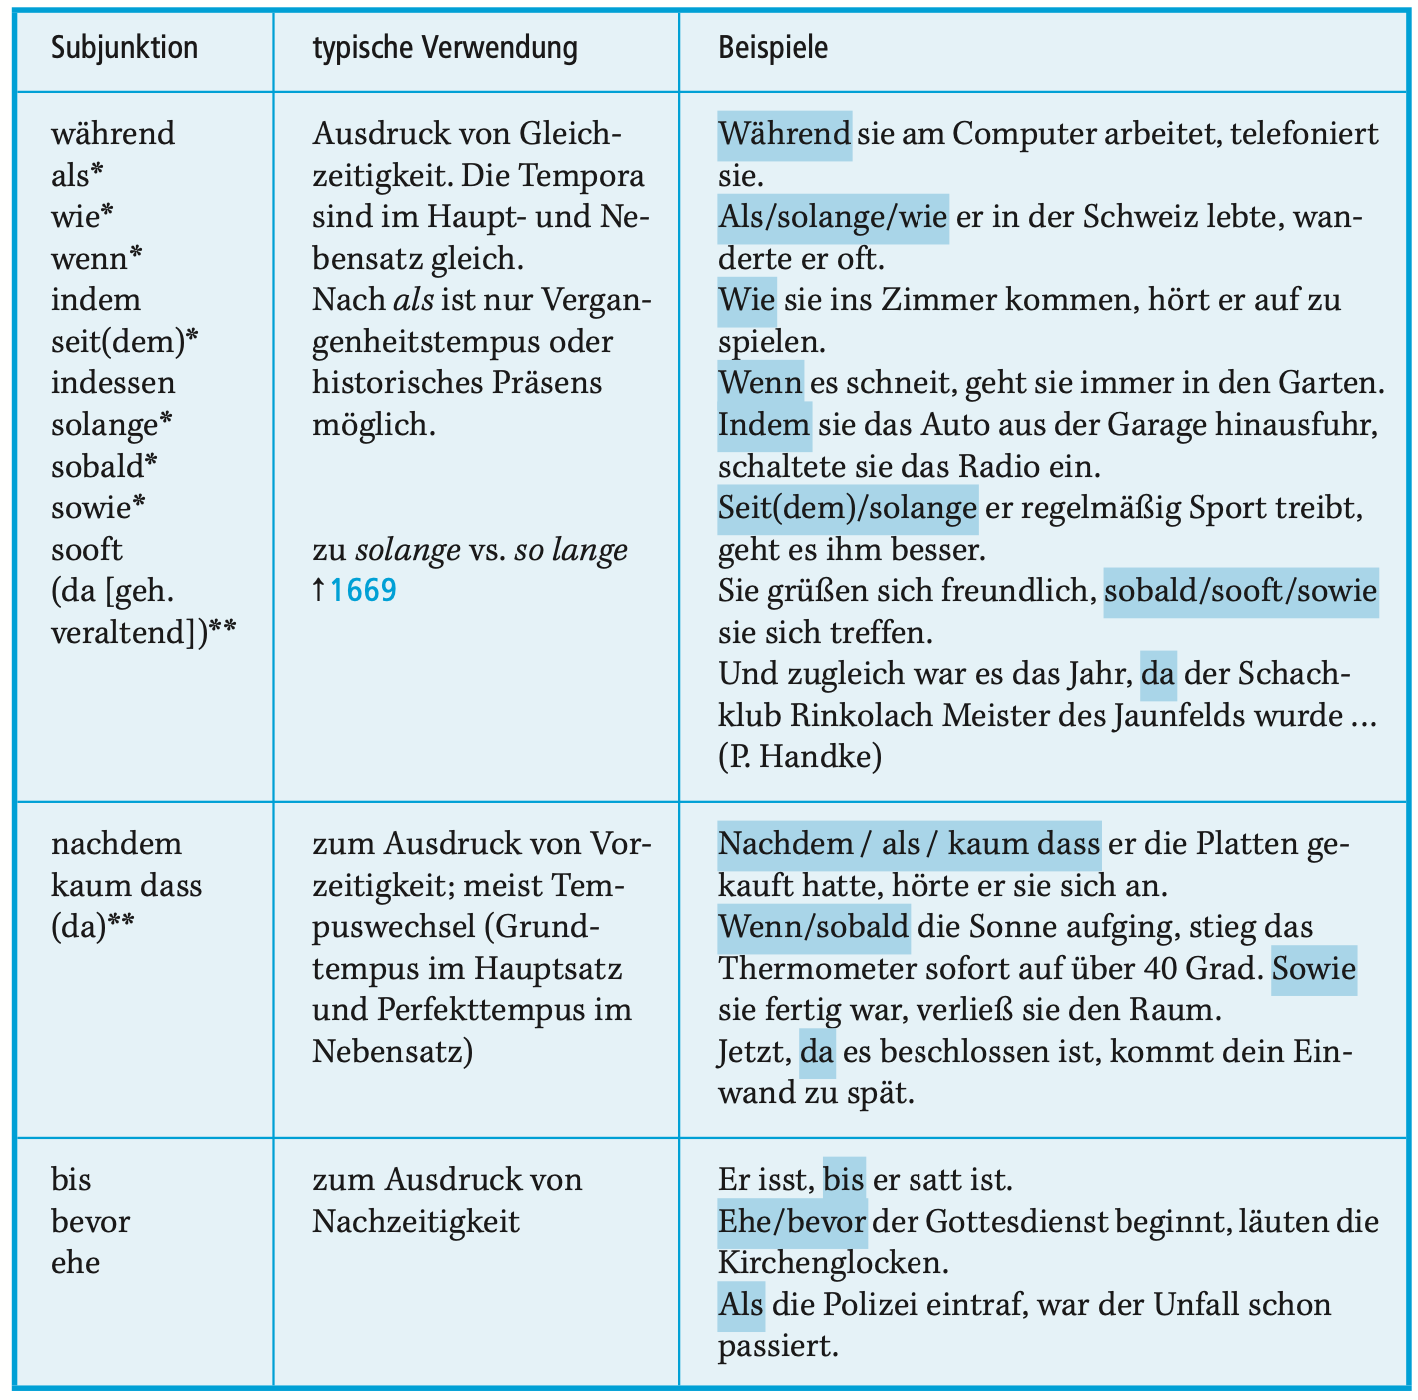
\includegraphics[scale=0.6]{tem.png}
\end{figure}

\subsection{Konditionale}
\begin{figure}[H]
    \centering
    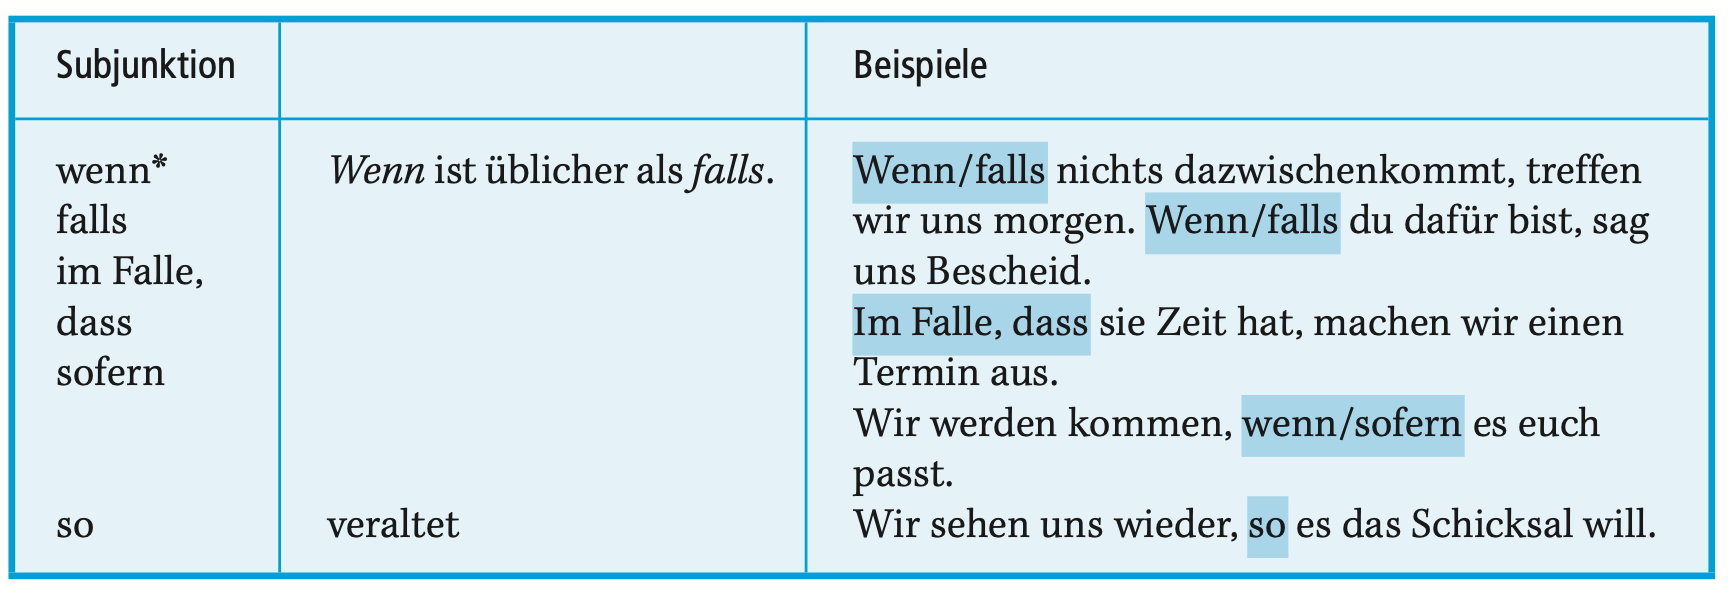
\includegraphics[scale=0.5]{kon1.png}
\end{figure}

\subsubsection{Irrelevanzkonditionale}
\begin{figure}[H]
    \centering
    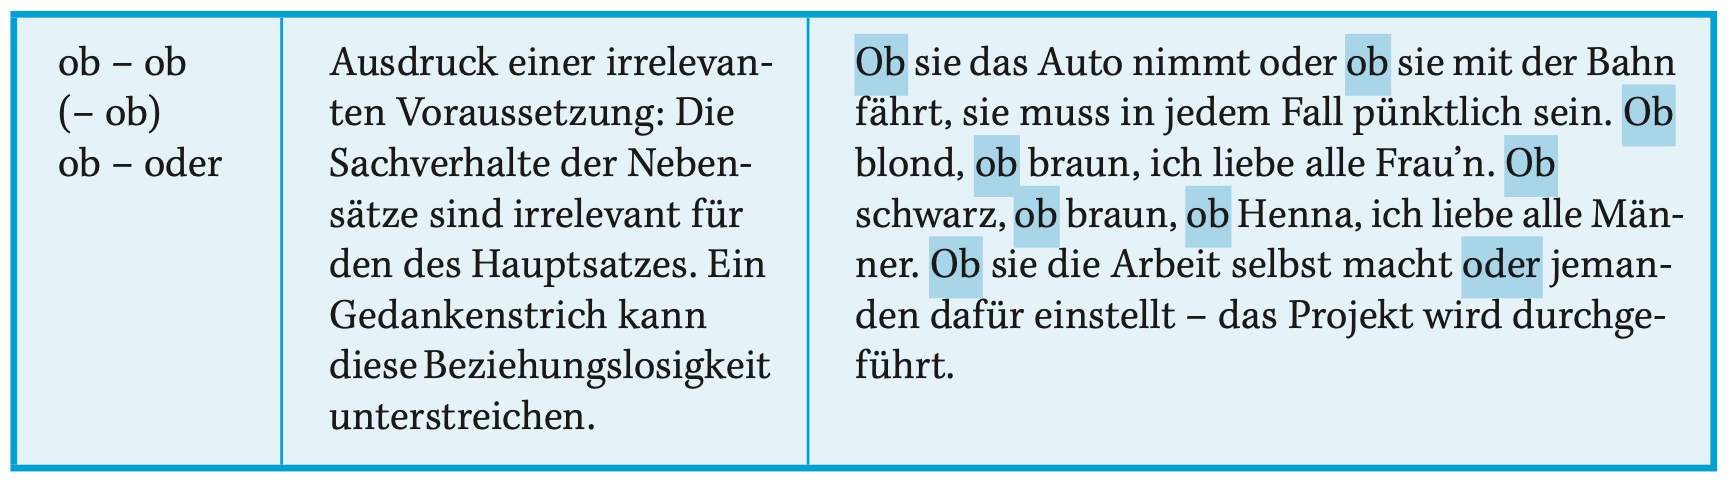
\includegraphics[scale=0.5]{kon2.png}
\end{figure}

\subsection{Adversative}
\begin{figure}[H]
    \centering
    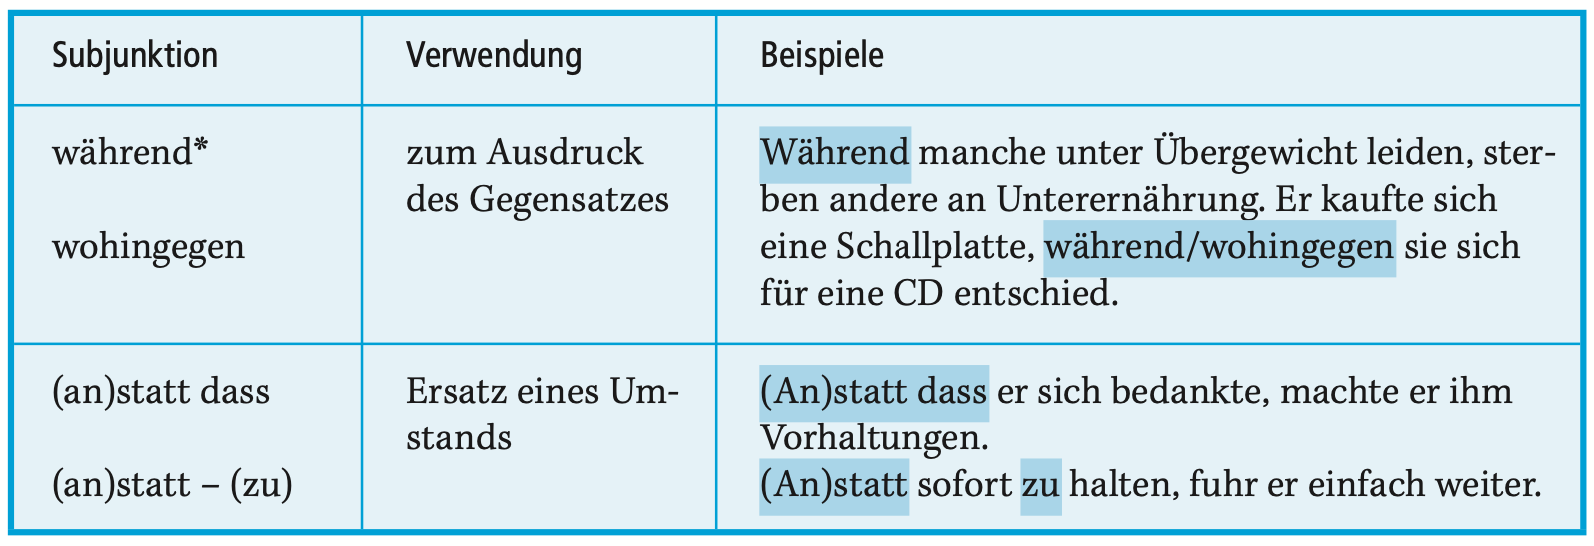
\includegraphics[scale=0.55]{ads.png}
\end{figure}



\subsection{Restriktive}
\begin{figure}[H]
    \centering
    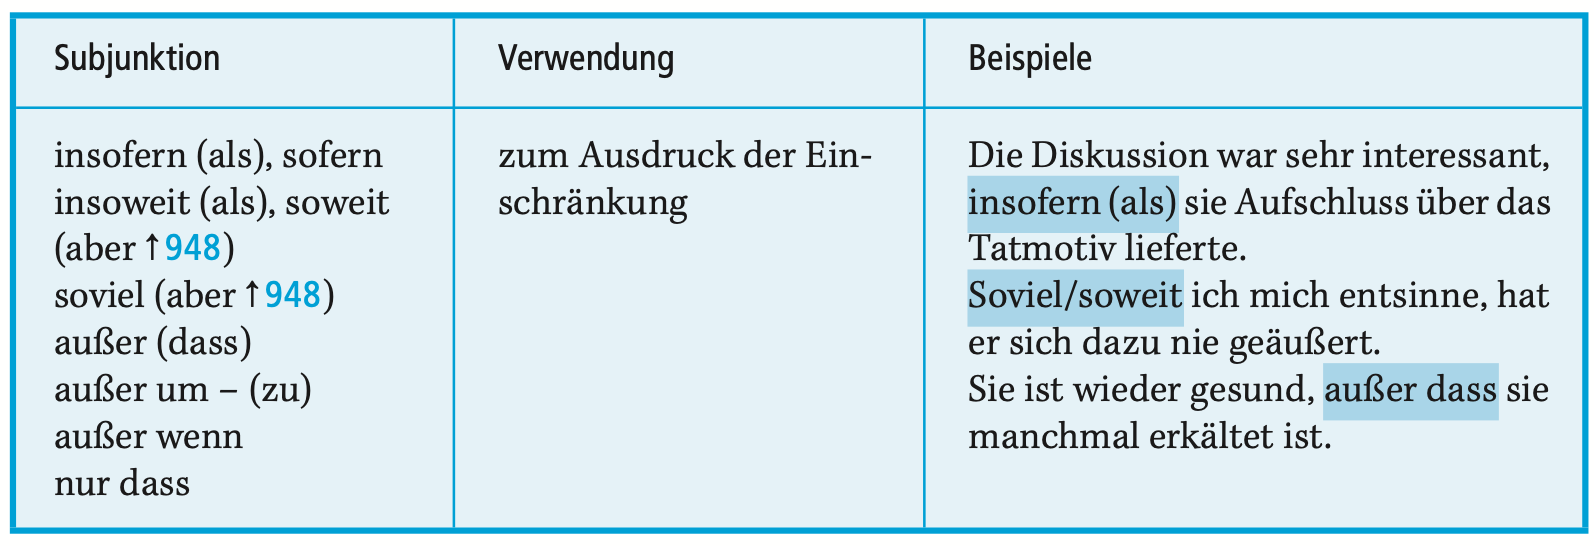
\includegraphics[scale=0.55]{res.png}
\end{figure}


\subsection{Vergleich}
\begin{figure}[H]
    \centering
    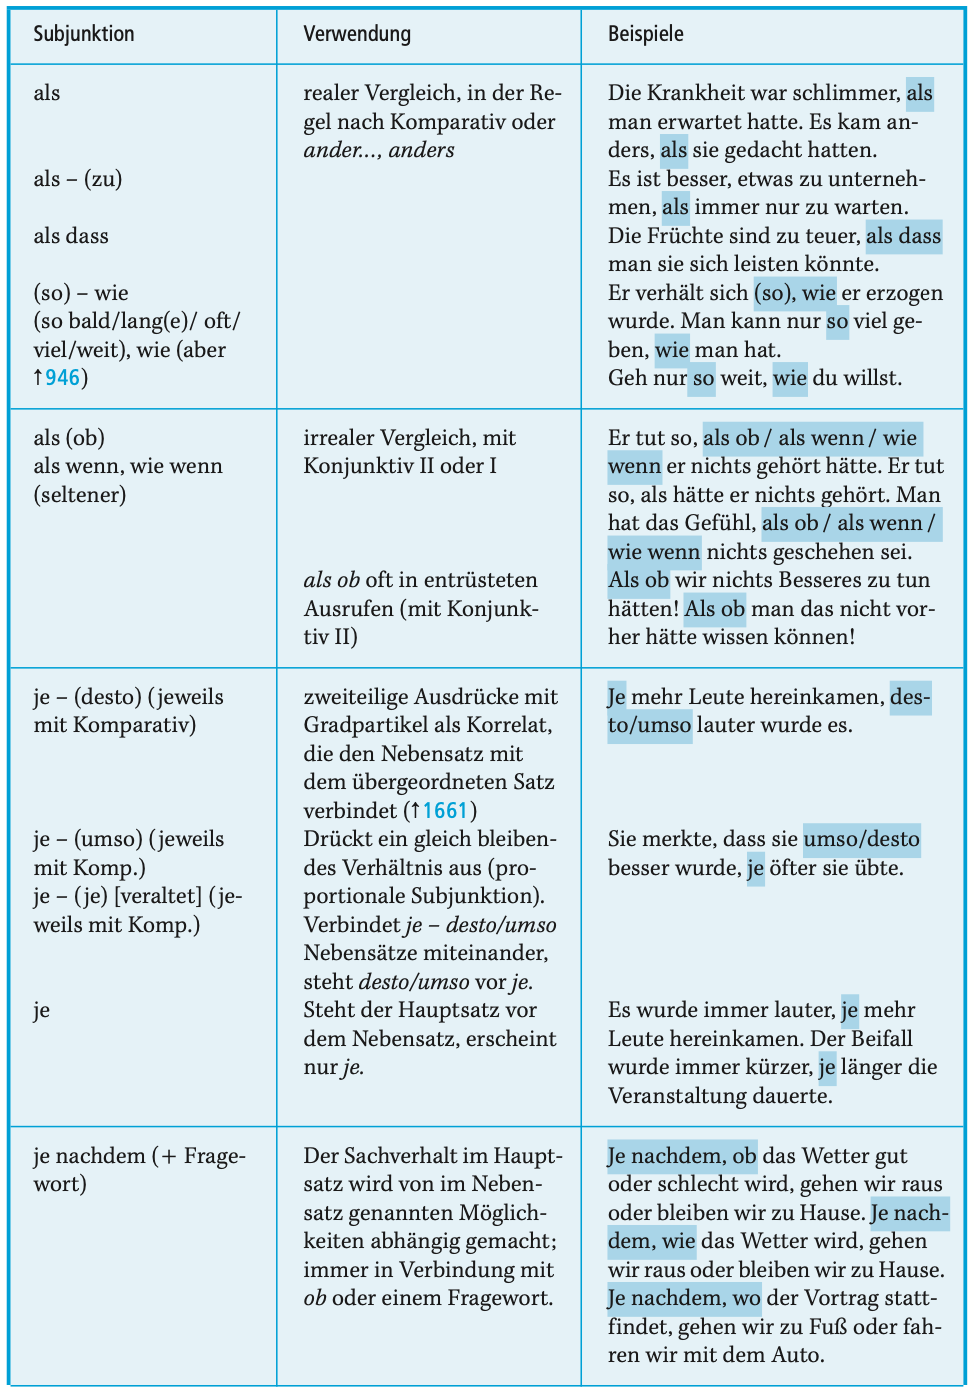
\includegraphics[scale=0.85]{verg.png}
\end{figure}

\subsection{Modal-instrumentale}
\begin{figure}[H]
    \centering
    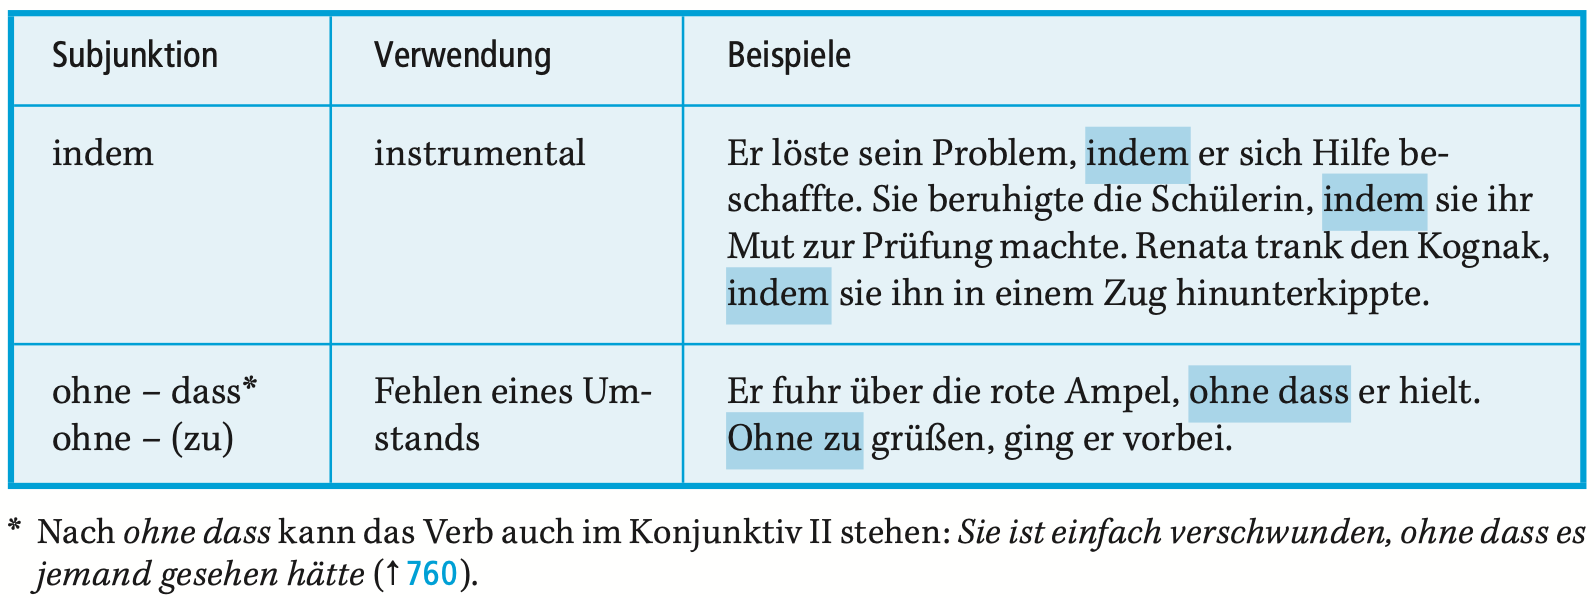
\includegraphics[scale=0.5]{mi.png}
\end{figure}


\subsection{Kasual}
\begin{figure}[H]
    \centering
    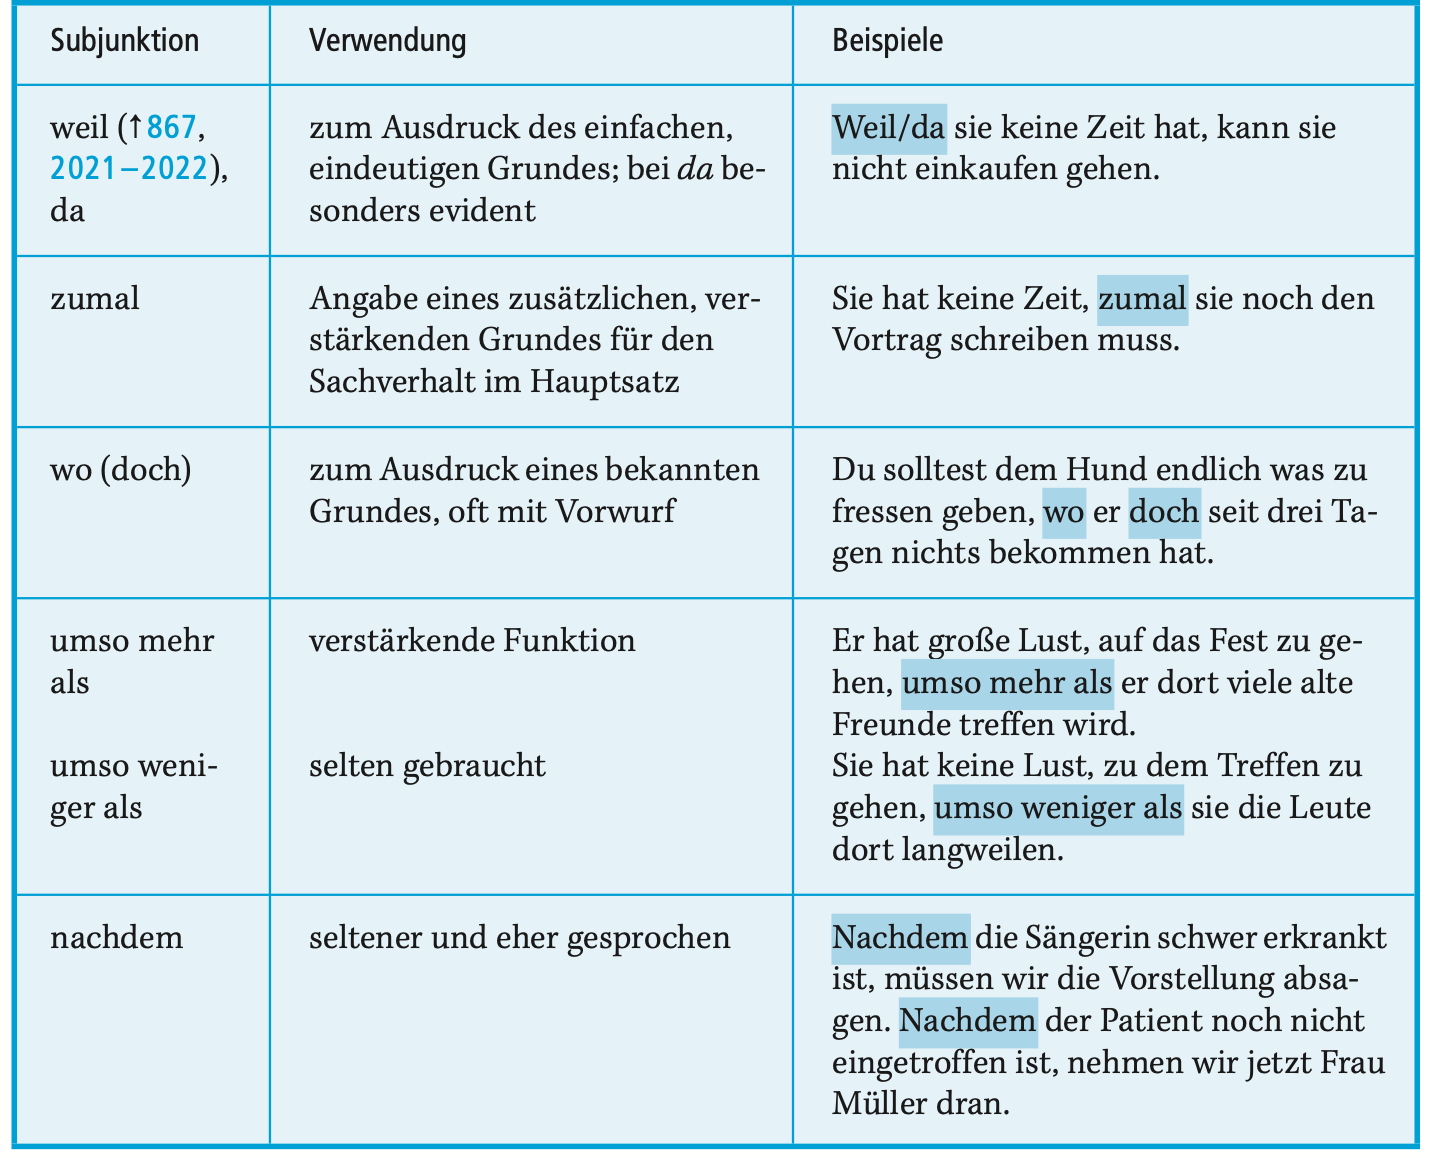
\includegraphics[scale=0.55]{kas.png}
\end{figure}

\subsection{Konsekutive}
\begin{figure}[H]
    \centering
    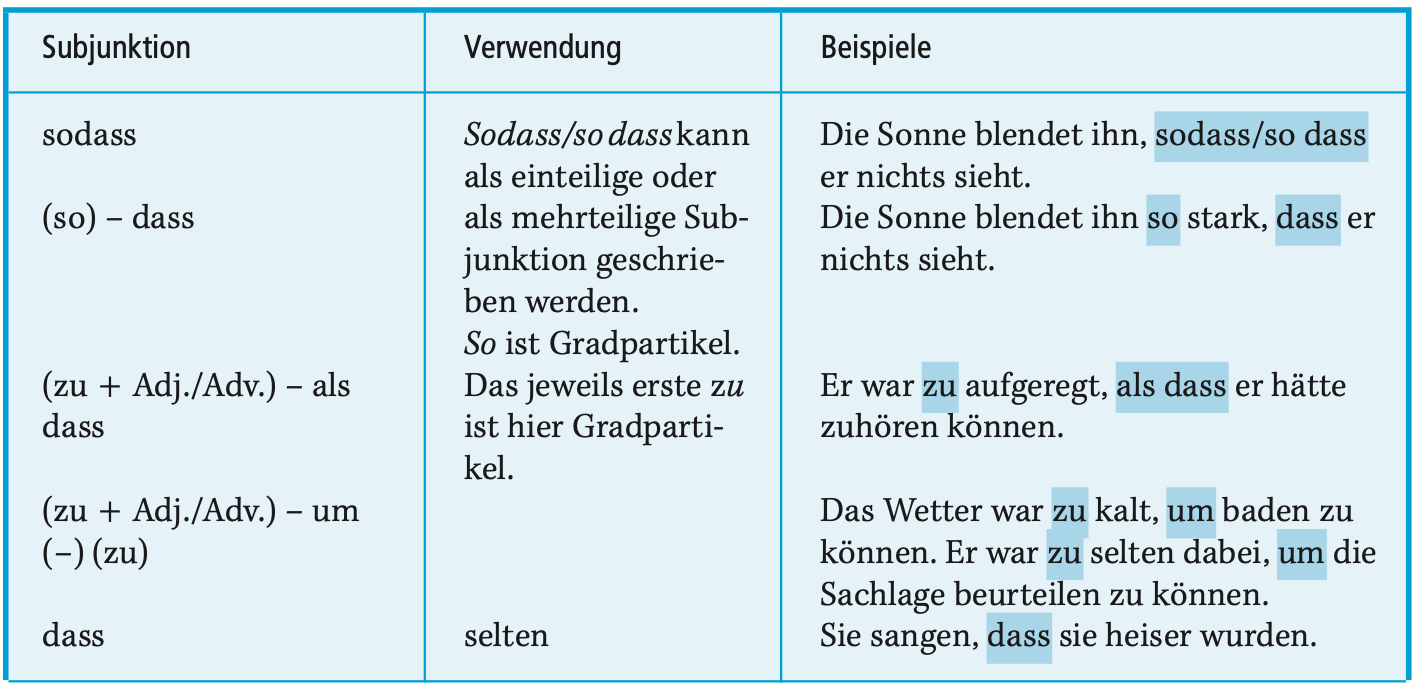
\includegraphics[scale=0.55]{se.png}
\end{figure}


\subsection{Final}
\begin{figure}[H]
    \centering
    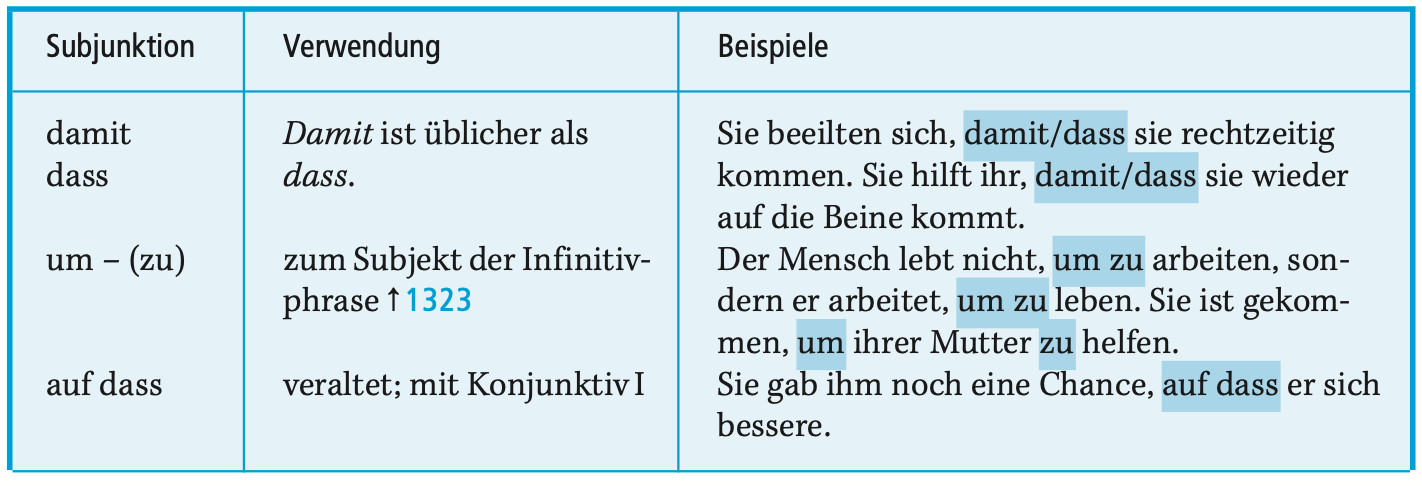
\includegraphics[scale=0.55]{fin.png}
\end{figure}

\subsection{Konzessive}
\begin{figure}[H]
    \centering
    \includegraphics[scale=0.55]{zes.png}
\end{figure}



\section{Liste}
\subsection{aber}
Konjunktion. Adversativ.
\subsection{allein}
Konjunktion. Adversativ.(=aber)


\subsection{als}
Subjunktion. 
\begin{enumerate}
    \item Temporal
    \begin{enumerate}
        \item Gleichzeitigkeit. Zeitpunkt. Einmaligkeit in der Vergangenheit
        \begin{itemize}
            \item Als der Verband gegründet wurde, zählte er nur wenige Mitglieder.
        \end{itemize}
        \item Vorzeitigkeit. Einmaligkeit in der Vergangenheit
        \begin{itemize}
            \item Als die Sonne aufgegangen war, begannen sie mit dem Bergauf stieg
            \item Als der Startschuß ertönte, sprangen die Schwimmer ins Wasser
        \end{itemize}
        \item Nachzeitigkeit
        \begin{itemize}
            \item Er hatte sich schlafen gelegt (kaum hatte er sich schlafen gelegt), als das Telefon klingelte
        \end{itemize}
    \end{enumerate}
    \item Modal
    \begin{enumerate}
        \item Komparativ. Realer Vergleich. Ungleichheit. 主句包含比较级/anders, auf andere Weise. NS immer Nachsatz
        \begin{itemize}
            \item Der gebrochene Arm ist schneller geheilt, als sie es sich selbst vorgestellt hat
            \item Er arbeitet anders, als du gearbeitet hast
            \item Der Mathematiker hat die Aufgabe auf andere Weise gelöst, als es der Gutachter vorgeschlagen hat
        \end{itemize}
        \begin{enumerate}
            \item als wenn. Hypothetischer Vergleich
            \begin{itemize}
                \item So ist es besser, als wenn wir es anders gemacht hätten
            \end{itemize}
        \end{enumerate}
        \item Komparativ. Hypothetischer Vergleich. Gleichheit. \textbf{Verberst}. NS immer Nachsatz
        \begin{itemize}
            \item Ich tat so, als sehe / sähe ich sie nicht
            \item Er hat den Eindruck, als sei / wäre / (ist) sie krank gewesen
            \item Die ausländische Studentin spricht (so gut) Deutsch, als sei / wäre sie eine Deutsche
        \end{itemize}
        \begin{enumerate}
            \item 这种Irrealität可通过祈使感叹句表达
            \begin{itemize}
                \item Als gäbe es außer dir niemanden, der im Ausland war
                \item Als lebten wir nicht im 20. Jahrhundert!
            \end{itemize}
        \end{enumerate}
        \item Modal. Spezifizierung. Mit kausaler Nebenbedeutung. 主句必须包含insofern / insoweit / um so + Komparativ(之所以是因为). NS immer Nachsatz
        \begin{itemize}
            \item Dieses Buch hat mich um so mehr interessiert, als darin meine Hei- mat beschrieben wird
            \item Das Buch war insofern interessant, als es eine Weiterentwicklung darstellte
            \item Diese Diskussion beschäftigte uns insoweit, als sie Einfluß auf unse- ren Betrieb hatte
            \item Er hatte um so weniger Anspruch auf ein höheres Gehalt, als er seine normalenVerpflichtungenkaumerfüllte
            \item Die Zusammenkunft war um so schöner, als alle Verwandten gekom- men waren
        \end{itemize}
    \end{enumerate}
\end{enumerate}

\subsection{als dass}
Subjunktion.
\begin{enumerate}
    \item Konsekutiv. 主句表示过量(zu + Adjektiv/Adjektivadverb/Partizip),从句表示期望的结果因此无法发生(太……以至于不能). NS immer Nachsatz
    \begin{itemize}
        \item Er ist zu krank, als daß er das Bett verlassen könnte
        \item Das Gebäude war zu zerstört, als daß man es hätte wieder aufbauen können
        \item Die Diskussion war zu interessant, als daß jemand nach Hause gegangen wäre
    \end{itemize}
    \begin{enumerate}
        \item 当主句和从句的主语相同时,用um + Infinitiv + zu结构
        \begin{itemize}
            \item Er ist zu krank, um das Bett verlassen zu können
        \end{itemize}
    \end{enumerate}
    \item Ersatz. 相比于从句中的事物更偏好主句中的事物(=anstatt daß). 主句中必须要有lieber / besser. NS immer Nachsatz
    \begin{itemize}
        \item Er fuhr lieber mit der Straßenbahn, als daß er den weiten Weg zu Fuß machte
    \end{itemize}
\end{enumerate}

\subsection{als ob}
Subjunktion. Modal. Hypothetischer Vergleich. Gleichheit(=als wenn, wie wenn). meist mit Konjunktiv. NS meist Nachsatz

\begin{itemize}
    \item Er tat, als ob er fest schlafe /schliefe /(schlief)
    \item Er erweckte den Eindruck, als ob er sehr überarbeitet sei /wäre
    \item Als ob wir nicht im 20. Jahrhundert lebten
    \item Als ob wir diese Entwicklung nicht schon lange vorausgeahnt hätten
\end{itemize}

\subsection{(an)statt dass/zu}
Subjunktion. Ersatz. 从句展示了一个未被选择的可能性,而主句则作为替代展示了另一种可能性. 主从句主语相同时用(an)statt + Infinitiv + zu
\begin{itemize}
    \item Er ging ins Theater, (an)statt daß er seinen Freund besuchte
    \item Er ging ins Theater, (an)statt seinen Freund zu besuchen
\end{itemize}

\subsection{außer daß}
Subjunktion
\begin{enumerate}
    \item Modal. Restriktiv(=nur daß)
    \begin{itemize}
        \item Er war geheilt, außer daß er in der Aufregung manchmal ein wenig stotterte.
    \end{itemize}
    \item 主从句主语相同时,用außer um zu
    \begin{itemize}
        \item Er ging nicht von ihrer Seite, außer um die Arzneimittel zu holen
    \end{itemize}
\end{enumerate}

\subsection{außer wenn}
Subjunktion.
\begin{enumerate}
    \item Restriktiv-konditional(除非)
    \begin{itemize}
        \item Er wird die Prüfung bestehen, außer wenn er sich nicht genügend vorbereitet.
        \item Ich gehe täglich spazieren, außer wenn es regnet
    \end{itemize}
    \item außer wenn $\ne$ wenn nicht
\end{enumerate}

\subsection{bevor}
Subjunktion
\begin{enumerate}
    \item Temporal. Nachzeitigkeit. Unmittelbare Aufeinanderfolge.(=ehe)
    \begin{itemize}
        \item Bevor er zur Arbeit geht, bringt er das Kind in den Kindergarten
    \end{itemize}
    \item 当主句带否定时,从句表示条件(bevor nicht = wenn nicht)从句加否定(fak.)不影响意思
    \begin{itemize}
        \item Er will den Arbeitsplatz nicht verlassen, bevor er (nicht) den Fehler an der Maschine gefunden hat
        \item Die Promovendin möchte ihre Dissertation nicht abschließen, bevor sie (nicht) alle Probleme gelöst hat
    \end{itemize}
\end{enumerate}


\subsection{beziehungsweise}
Konjunktion. Alternativ. (= oder)
\begin{itemize}
    \item Er will kommen, bzw. sie will anrufen
    \item Er bzw. seine Frau wird herkommen
\end{itemize}


\subsection{bis}
Subjunktion. Temporal. Nachzeitigkeit. Endpunkt. Ziel
\begin{itemize}
    \item Ich warte auf dich, bis du wiederkommst
    \item Bis der Regen aufhört, bleibst du hier
    \item Bis die Arbeit fertig ist, können wir nicht nach Hause gehen
\end{itemize}

\subsection{da}
Subjunktion. Kausal. 从句是原因
\begin{itemize}
    \item Da es heute regnet, nimmt er einen Schirm
    \item Er konnte gestern die Versammlung nicht besuchen, da er krank war
\end{itemize}

\subsection{damit/um……zu}
Subjunktion. Final. 从句是目的主句是前提. 主从句主语相同时用um……zu
\begin{itemize}
    \item Er schenkte ihr Briefpapier, damit sie ihm öfter schriebe
    \item Er fährt an die Ostsee, um sich zu erholen
\end{itemize}

\subsection{das heißt}
Konjunktion. Spezifizierung
\begin{itemize}
    \item Wir reisen morgen in die Schweiz, d.h., wir fahren nach Zürich
\end{itemize}

\subsection{denn}
Konjunktion. 第二个分句给第一个分句提供原因
\begin{itemize}
    \item Wir gehen spazieren, denn das Wetter ist schön
    \item Das Arbeitsergebnis war ausgezeichnet, denn alle Mitarbeiter haben sich sehr angestrengt
\end{itemize}

\subsection{doch}
Konjunktion(=jedoch, aber)
\begin{itemize}
    \item Wir wollten ihn besuchen, doch er war nicht zu Hause
\end{itemize}

\subsection{ehe}
Subjunktion. 
\begin{enumerate}
    \item Temporal. Nachzeitigkeit. (=bevor)
    \begin{itemize}
        \item Ehe er zur Arbeit geht, bringt er das Kind in den Kindergarten
    \end{itemize}
    \item Ersatz. 更偏好主句中的事物(=anstatt daß)
    \begin{itemize}
        \item Ehe er den weiten Weg zu Fuß machte, fuhr er lieber mit der Straßenbahn
    \end{itemize}
\end{enumerate}


\subsection{entweder……oder}
Konjunktion. Alternativ

\begin{itemize}
    \item Entweder wir gehen ins Kino, oder wir besuchen unsere Freunde
    \item Du weißt, daß du entweder die Prüfung bestehen mußt oder daß du nicht mehr weiterstudieren kannst
\end{itemize}

\subsection{falls}
Subjunktion. Konditional(=wenn)
\begin{itemize}
    \item Er wird uns besuchen, falls er nach Leipzig kommt
\end{itemize}

\subsection{indem}
Subjunktion. Modal. Instrumental. 从句表示工具,主句表示目的(=dadurch daß)
\begin{itemize}
    \item Er beruhigte das Kind, indem er es streichelte
    \item Man setzt diese Maschine in Betrieb, indem man den rechten Hebel herunterdrückt
    \item Indem er mit dem Kind rechnete, half er ihm, die Prüfung zu beste- hen
\end{itemize}

\subsection{insofern/insoweit(als)}
Subjunktion. Modal. Spezifizierung.
\begin{itemize}
    \item Der Abend war interessant, insofern (als) es die musikalischen Darbietungen betraf
    \item Die Dissertation war ausgezeichnet, insoweit (als) sie theoretische Fragestellungen behandelte
\end{itemize}

\subsection{je……desto/umso}
Subjunktion. NS gewöhnlich als V ordersatz
\begin{enumerate}
    \item 当该词组处于从句中时,je引导的句子在desto后
    \begin{itemize}
        \item Er merkte, daß er um so besser spielen konnte, je öfter er übte
    \end{itemize}
    \item je引导的从句在后时,主句的desto/umso可换成immer,也可用und
    \begin{itemize}
        \item Er wurde immer lustiger, je mehr er trank
        \item Das Auto fuhr schneller und schneller, je steiler der Abhang wurde
    \end{itemize}
\end{enumerate}


\subsection{je nachdem}
Subjunktion. 主句的事件取决于从句不同情况的可能性. 总与ob或疑问词相连
\begin{itemize}
    \item Je nachdem ob das Wetter schön oder schlecht ist, gehen wir spazieren oder bleiben wir zu Hause
    \item Wir gehen spazieren oder bleiben zu Hause, je nachdem wie das Wetter ist.
\end{itemize}

\subsection{jedoch}
Konjunktion
\begin{itemize}
    \item Wir gehen fort, jedoch ihr bleibt zu Hause
\end{itemize}

\subsection{kaum daß}
Subjunktion. Temporal. Vorzeitigkeit. Unmittelbare Aufeinanderfolge
\begin{itemize}
    \item Kaum daß das Klingelzeichen ertönt war, strömten die Kinder aus dem Klassenzimmer
    \item Sie begannen zu essen, kaum daß das Essen auf dem Tisch stand
\end{itemize}

\subsection{nachdem}
Subjunktion. Temporal. Vorzeitigkeit. 从句若用过去完成式,主句要用过去时;从句用现在完成时,主句要用现在时或将来时
\begin{itemize}
    \item Nachdem wir in der Stadt angekommen waren, suchten wir uns ein Hotelzimmer
    \item Nachdem wir in der Stadt angekommen sind, suchen wir uns ein Ho- telzimmer
    \item Nachdem wir mit ihm gesprochen haben, werden wir seine Angelegenheit klären
\end{itemize}

\subsection{nicht nur……sondern auch}
Konjunktion.(= und zusätzlich auch)
\begin{itemize}
    \item Er hat nicht nur ein Hochschulstudium abgeschlossen, sondern (er hat) auch promovier
\end{itemize}

\subsection{nur daß}
Subjunktion. Modal. Restriktiv. NS immer als Nachsatz
\begin{itemize}
    \item Er verfügte über ein umfangreiches Fachwissen, nur daß er noch nicht genügend Erfahrung gesammelt hatt
\end{itemize}

\subsection{ob}
Subjunktion. ob-Satz可像dass-Satz那样作为主句的主语/宾语

\subsection{ob……order}
Konzessiv. 从句的各种可能性与主句无关. 从句在前时,主句此时是Verbzweit
\begin{itemize}
    \item Wir gingen spazieren, ob es regnete oder die Sonne schien
    \item Ob es regnet oder die Sonne scheint, wir gehen (doch) spazieren
    \item Ob er es will oder nicht, mit diesem Resultat muß er rechnen
\end{itemize}


\subsection{obwohl}
Subjunktion. 从句在前时,主句添加(fak.) so (in Spitzenstellung) und doch (nach finitem Verb und Subjekt) 

\begin{itemize}
    \item Er arbeitet noch, obwohl er schon alt ist
    \item Obwohl er schon alt ist, (so) arbeitet er (doch) noch
\end{itemize}


\subsection{ohne daß/zu}
Subjunktion. 主从句主语(逻辑主语而不是语法主语)相同时用zu
\begin{enumerate}
    \item Modal. Fehlender Begleitumstand
    \begin{itemize}
        \item Er ging durch den Regen, ohne daß er den Regenschirm aufspannte
    \end{itemize}
    \item Konsekutiv. 从句陈述了主句预期结果未发生
    \begin{itemize}
        \item Sie litt unter schweren Schmerzen, ohne darüber zu klagen
        \item Sie schrie vor Schmerzen, ohne daß der Arzt ihr hätte helfen können
    \end{itemize}
\end{enumerate}

\subsection{seit(dem)}
Subjunktion. Temporal
\begin{enumerate}
    \item Gleichzeitigkeit. Zeitdauer bis Sprechergegenwart mit Anfangspunkt in der Vergangenheit. 只用现在时或过去时的持续动词
    \begin{itemize}
        \item Seit(dem) ich ihn kenne, ist er Nichtraucher
        \item Seit(dem) sie auf dem Lande wohnte, ging es ihr besser
    \end{itemize}
    \item Vorzeitigkeit. Genauer Anfangspunkt in der Vergangenheit. 只用完成时
    \begin{itemize}
        \item Seit(dem) er aus dem Krankenhaus entlassen ist, arbeitet er in einem anderen Betrieb
        \item Seit(dem) seine Frau gestorben war, ging er zu keiner Veranstaltung mehr
    \end{itemize}
\end{enumerate}


\subsection{so daß}
Subjunktion. Konsekutiv. 从句是结果

\begin{itemize}
    \item Es war kalt, so daß wir froren
    \item In der Nacht hatte es geregnet, so daß die Waldwege schlammig wa- ren.
\end{itemize}


\subsection{sobald}
Subjunktion. Temporal. sowie
\begin{enumerate}
    \item Vorzeitigkeit. Unmittelbare Aufeinanderfolge(=als, kaum daß)
    \begin{itemize}
        \item Sobald (sowie) sie ihren Freund sah (gesehen hatte), eilte sie auf ihn zu.
        \item Sobald der Zug ankommt (ankommen wird), werden wir anrufen
    \end{itemize}
    \item Gleichzeitigkeit(=wenn)
    \begin{itemize}
        \item Sobald es läutet (läutete), setzen (setzten) sich die Schüler auf ihre Plätze
        \item Sobald er in Dresden ist, sucht er seinen Freund auf
    \end{itemize}
\end{enumerate}


\subsection{sofern}
Subjunktion. Konditional(=wenn, falls)
\begin{itemize}
    \item Wir werden den Zug noch erreichen, sofern wir uns beeilen
    \item Sofern du mir hilfst, schaffe ich die Prüfung
\end{itemize}

\subsection{solange}
Subjunktion. Temporal. Gleichzeitigkeit. Zeitdauer mit gleichem Beginn und gleichem Ende

\begin{itemize}
    \item Ich bleibe hier, solange du hier bist
    \item Solange es Kriege gibt, ist die Existenz der Völker bedroht
    \item Er gönnte sich keine Ruhe, solange er an dem Buch schrieb
\end{itemize}

\begin{enumerate}
    \item synonyme Formen:so lang在主句作为Korrelat,wie引导从句
    \begin{itemize}
        \item Ich bleibe so lange hier, wie du hier bist
    \end{itemize}
\end{enumerate}

\subsection{sondern}
Subjunktion. Adversativ
\begin{itemize}
    \item Er kaufte sich für das Geld kein Auto, sondern er machte eine Reise
    \item Wir gingen nicht ins Kino, sondern ins Theater
\end{itemize}

\subsection{sooft}
Subjunktion. Temporal. Wiederholung. 主句的事件根据从句事件反复发生(=jedesmal wenn)
\begin{enumerate}
    \item Gleichzeitigkeit
    \begin{itemize}
        \item Sooft er zu Hause war, freuten sich die Kinder
        \item Er grüßt mich freundlich, sooft er mich trifft
    \end{itemize}
    \item orzeitigkeit
    \begin{itemize}
        \item Sooft er nach Hause kam, freuten sich die Kinder.
        \item Er erkältete sich, sooft er bei kühlem Wetter badete
    \end{itemize}
\end{enumerate}


\subsection{soviel/soweit}
Subjunktion

\begin{enumerate}
    \item Modal. Restriktiv. 从句对主句陈述进行主观性限定(据……所知)
    
    \begin{itemize}
        \item Soviel ich gehört habe, ist er krank
        \item Es handelt sich um einen Unfall, soviel man sieht
        \item Soweit ich das Buch beurteilen kann, handelt es sich um eine Arbeit von internationaler Bedeutung
        \item Er wird die Prüfung sehr gut bestehen, soweit ich ihn kenne
    \end{itemize}
    \item soviel加上auch,表示让步
    \begin{itemize}
        \item Der Student schafft es nicht, soviel er auch arbeitet = obwohl er viel arbeitet
    \end{itemize}
\end{enumerate}

\subsection{sowie}
\begin{enumerate}
    \item sobald
    \item und
\end{enumerate}

\subsection{sowohl als/wie auch}
Konjunktion. Kopulativ. (= und)
\begin{itemize}
    \item Er ist sowohl Arzt als auch (wie auch) Künstler
    \item Seine Arbeiten sind sowohl wissenschaftlich neu als auch (wie auch) verständlich geschrieben
\end{itemize}


\subsection{(an)statt}
不连接主从句
\begin{itemize}
    \item Er schrieb mir (an)statt ihm
    \item Wir tranken Tee (an)statt Kaffee
\end{itemize}


\subsection{trotzdem}
Subjunktion. Konzessiv. (= obwohl)
\begin{itemize}
    \item Trotzdem mehrere Spieler verletzt waren, hat die Mannschaft das entscheidende Spiel gewonnen
\end{itemize}


\subsection{um so mehr/weniger als}
Subjunktion. Kausa. 从句为主句提供额外的更强的理由(=zumal)

\begin{itemize}
    \item Er geht selten ins Kino, um so weniger als er keine Zeit hat.
    \item Er geht oft ins Kino, um so mehr als er keinen Fernseher hat
\end{itemize}

\subsection{um……zu}
\begin{enumerate}
    \item Final. 替代damit
    \begin{itemize}
        \item Er fährt an die Ostsee, um sich zu erholen
    \end{itemize}
    \item Konsekutiv. 替代dass/als dass
    \begin{itemize}
        \item Das Wasser war zu kalt, als daß man darin baden konnte
        
        -> Das Wasser war zu kalt, um darin baden zu können
        \item Das Wasser war so kalt, daß man nicht darin baden konnte
        
        -> Das Wasser war zu kalt, um darin baden zu können
    \end{itemize}
    \item Konditional. 替代wenn
    \begin{itemize}
        \item Er muß fleißig sein, wenn er die Prüfung bestehen will
        
        ->  Er muß fleißig sein, um die Prüfung zu bestehen
    \end{itemize}
    \item Kopulativ. 替代und
    \begin{itemize}
        \item Er betrat das Lokal und verließ es nach einer Stunde wieder
        
        -> Er betrat das Lokal, um es nach einer Stunde wieder zu verlassen
    \end{itemize}
\end{enumerate}

\subsection{während}
Subjunktion
\begin{enumerate}
    \item Temporal. Gleichzeitigkeit. Zeitdauer
    \item Adversativ
    \begin{itemize}
        \item Während es gestern schön war, ist das Wetter heute schlecht
        \item Während er die Prüfung bereits bestanden hat, hat sie sie noch nicht bestanden.
    \end{itemize}
\end{enumerate}


\subsection{weder……noch}
(= nicht... und auch nicht)
\begin{itemize}
    \item ch habe ihn weder besucht, noch habe ich ihm geschrieben.
\end{itemize}

\subsection{weil}
Subjunktion

\subsection{wenn}
Subjunktion
\begin{enumerate}
    \item Temporal
    \begin{enumerate}
        \item Gleichzeitigkeit. Zeitpunkt. Einmaliges Geschehen in Gegenwart und Zukunft(als是过去)
        \begin{itemize}
            \item Der Unterricht ist zu Ende, wenn das Klingelzeichen ertönt
            \item Wenn die Sonne am höchsten steht, ist Mittag
        \end{itemize}
        \item Gleichzeitigkeit. Zeitpunkt. Wiederholtes Geschehen ( = jedesmal wenn, immer wenn)
        \begin{itemize}
            \item Wenn es regnete, blieben wir zu Hause
            \item Wenn es läutet, setzen sich die Schüler auf ihre Plätze
        \end{itemize}
        \item Vorzeitigkeit. Abschluß eines Geschehens.
        \begin{itemize}
            \item Er liest die Zeitung, wenn er gefrühstückt hat
            \item Wenn der Besuch gekommen ist, beginnen wir mit dem Essen
        \end{itemize}
    \end{enumerate}
    \item Konditional (=falls)
    \begin{enumerate}
        \item 从句表示条件,主句表示结果
        \begin{itemize}
            \item Wenn das Wetter schön ist, gehen wir spazieren.
        \end{itemize}
        \begin{enumerate}
            \item 如果表示非现实条件,则wenn后动词用Konjuntiv
        \end{enumerate}
    \end{enumerate}
    \item Isolierte Wunschsätze. Indikativ und Konjunktiv(如果……就好了)
    \begin{itemize}
        \item Wenn doch der Briefträger käme!
        \item Wenn er nur zu uns kommt!
    \end{itemize}
\end{enumerate}


\subsection{wenn auch so doch}
Subjunktion. Konzessiv. wenn auch引导从句,so doch引导主句. 主句在前时,so必须删去
\begin{itemize}
    \item Wenn auch einige nicht dabei waren, so war es doch ein unterhaltsamer Abend
    \item Es war (doch) ein unterhaltsamer Abend, wenn auch einige nicht dabei waren.
    \item Wenn es auch kalt ist, so zieht er doch keinen Mantel an
    \item Wenn er die Prüfung auch nicht besonders gut abgelegt hat, so war er doch fleißig
\end{itemize}


\subsection{wie}
Subjunktion. Modal. Komparativ. Realer Vergleich. Gleichheit(正如)
\begin{enumerate}
    \item 方式的比较. so作为Korrelat(fak.)
    \begin{itemize}
        \item Der Dozent hat (so) geprüft, wie ich es mir vorgestellt hatte
        \item Er macht seine Arbeit (so), wie er sie immer gemacht hat
    \end{itemize}
    \item 程度的比较. so作为Korrelat(obl.)
    \begin{itemize}
        \item Er ist so alt, wie ich bin
    \end{itemize}
\end{enumerate}

\subsection{wie auch}
Subjunktion. Konzessiv. mit immer(fak.)从句在前时,主句此时是Verbzweit
\begin{itemize}
    \item Sie konnten den Berg nicht ersteigen, wie sehr sie sich auch (immer) anstrengte
    \item Wie morgen das Wetter auch sein mag, wir müssen verreisen
\end{itemize}

\subsection{zumal}
Subjunktion. Kausal. Zusätzlicher Grund.
\begin{itemize}
    \item Der Lehrer lobte den Schüler, zumal sich dessen Leistungen schon seit längerer Zeit verbesserten
\end{itemize}

\chapter{Konnektoren}
\section{Kopulative}
\subsection{Additive}
\begin{longtable}{|>{\raggedright\arraybackslash}p{1cm}|>{\raggedright\arraybackslash}p{12cm}|}

\hline
\textbf{Präp} & \textit{einschließlich, samt, nebst, inklusive, zuzüglich, mit, bei} \\
\hline
\textbf{Subj} & \textit{(nicht) ohne dass; (nicht) ohne zu} \\
\hline
\textbf{Konj} & \textit{und; sowie; sowohl -- wie/als (auch); nicht nur/allein/bloß -- sondern auch; (weder -) noch geschweige denn} \\
\hline
\textbf{Rel} & \textit{wie auch, wobei} \\
\hline
\textbf{Adv} & \textit{auch, ferner, außerdem, weiterhin, darüber hinaus, gleichfalls, ebenfalls, zudem, überdies, ebenso, zusätzlich, dazu, dabei, übrigens, im Übrigen, des Weiteren, nicht zuletzt, vor allem, insbesondere; erstens -- zweitens; letztlich, schließlich} \\
\hline
\textbf{Abt} & \textit{auch} \\
\hline
\end{longtable}

\begin{enumerate}
    \item Relativkonstruktionen使用Verbletztstellung
    \begin{itemize}
        \item Wie auch die Panade keine künstlichen Farbstoffe und Geschmacksverstärker enthalten soll
    \end{itemize}
\end{enumerate}

\subsection{Alternative}

\begin{longtable}{|>{\raggedright\arraybackslash}p{1cm}|>{\raggedright\arraybackslash}p{12cm}|}
\hline
\textbf{Konj} & \textit{oder, beziehungsweise, bzw., entweder -- oder (auch)/(aber)}\\
\hline
\end{longtable}

\section{Temporal}
\subsection{Vorzeitige}
\begin{longtable}{|>{\raggedright\arraybackslash}p{1cm}|>{\raggedright\arraybackslash}p{12cm}|}

\hline
\textbf{Präp} & \textit{nach} \\
\hline
\textbf{Subj} & \textit{nachdem, kaum, dass} \\
\hline
\textbf{Rel} & \textit{wonach, worauf} \\
\hline
\textbf{Adv} & \textit{dann, danach, sodann, darauf(hin), anschließend, alsdann, nachher, bald, sofort, nun, schon, seitdem, schließlich, endlich, später} \\
\hline

\end{longtable}

\subsection{Nachzeitige}
\begin{longtable}{|>{\raggedright\arraybackslash}p{1cm}|>{\raggedright\arraybackslash}p{5.5cm}|>{\raggedright\arraybackslash}p{5.5cm}|}
\hline
\textbf{} & \textbf{auf einen Zeitpunkt bezogen} & \textbf{auf eine Zeitdauer bezogen} \\
\hline
\endfirsthead

\hline
\textbf{} & \textbf{auf einen Zeitpunkt bezogen} & \textbf{auf eine Zeitdauer bezogen} \\
\hline
\endhead

\textbf{Präp} & \textit{vor} & \textit{bis} \\
\hline
\textbf{Subj} & \textit{bevor, ehe} & \textit{bis} \\
\hline
\textbf{Adv} & \textit{vorher, davor, früher, zuvor, vordem, einst, zunächst} & \textit{bis dahin, bislang} \\
\hline

\end{longtable}


\subsection{Gleichzeitige}
\begin{adjustbox}{width=\textwidth}
\begin{tabular}{|>{\raggedright\arraybackslash}p{1cm}|
                >{\raggedright\arraybackslash}p{2.8cm}|
                >{\raggedright\arraybackslash}p{2.8cm}|
                >{\raggedright\arraybackslash}p{2.8cm}|
                >{\raggedright\arraybackslash}p{2.8cm}|
                >{\raggedright\arraybackslash}p{2.8cm}|}
\hline
\textbf{} &
\textbf{im Verlauf} &
\textbf{im Verlaufs\-abschluss} &
\textbf{mit Verlaufs\-beginn} &
\textbf{auf Eintritt bezogen} &
\textbf{wiederholt (iterativ)} \\
\hline
\textbf{Präp} &
\textit{während, bei, zu, binnen, durch} & 
& 
\textit{seit} & 
\textit{mit, bei} & 
\\
\hline
\textbf{Subj} &
\textit{während, als, wie, wenn, indem} &
\textit{solange} &
\textit{seit, seitdem} &
\textit{sobald, sowie, erst als / wenn / wie, kaum/gerade -- als, als gerade} &
\textit{(immer) wenn, sooft} \\
\hline
\textbf{Rel} &
\textit{wo, da, wann, wenn} &
 & 
 & 
 & 
 \\
\hline
\textbf{Adv} &
\textit{währenddessen, gleichzeitig, zugleich, damals} &
\textit{solange} &
\textit{seitdem, seither, inzwischen, derweil, unterdessen} &
\textit{da, plötzlich, soeben, gerade} &
\textit{jedesmal, immer} \\
\hline
\end{tabular}
\end{adjustbox}

\section{Konditionale}
\begin{longtable}{|>{\raggedright\arraybackslash}p{1cm}|>{\raggedright\arraybackslash}p{12cm}|}

\hline
\textbf{Präp} & \textit{bei, unter, mit, im Fall(e) (von)} \\
\hline
\textbf{Subj} & \textit{wenn, falls, (in)sofern; sobald, bevor/ehe nicht; ob} \\
\hline
\textbf{Adv} & \textit{sonst, andernfalls, ansonsten, dann, unter Umständen, eventuell} \\
\hline

\end{longtable}

\begin{enumerate}
    \item 主句中的Korrelat为dann/so
    \begin{itemize}
        \item Wenn Bäume in Gefahr sind zu sterben, (dann/so) produzieren sie ungewöhnlich viele Früchte
    \end{itemize}
\end{enumerate}

\section{Kausale}

\subsection{Im engeren Sinne Kausale}
\begin{longtable}{|>{\raggedright\arraybackslash}p{1cm}|>{\raggedright\arraybackslash}p{12cm}|}

\hline
\textbf{Präp} & \textit{wegen, aufgrund (von), aus, vor, durch, dank, qua, infolge, gemäß, kraft, mangels, anlässlich, angesichts; halber, zuliebe, zufolge; um [...] willen} \\
\hline
\textbf{Subj} & \textit{weil, da (doch); um so [...] als, um so mehr als, um so weniger als, zumal (da), insofern -- als} \\
\hline
\textbf{Konj} & \textit{denn} \\
\hline
\textbf{Rel} & \textit{weswegen, weshalb, warum} \\
\hline
\textbf{Adv} & \textit{deshalb, daher, darum, also, deswegen, darum, demnach, demgemäß, dadurch, infolgedessen, dementsprechend, aus diesem Grund} \\
\hline
\textbf{Abt} & \textit{ja, doch, eben} \\
\hline
\end{longtable}


\subsection{Konsekutive}
\begin{longtable}{|>{\raggedright\arraybackslash}p{1cm}|>{\raggedright\arraybackslash}p{12cm}|}

\hline
\textbf{Präp} & \textit{auf [...] hin, infolge} \\
\hline
\textbf{Subj} & \textit{sodass; so [...] / dermaßen [...] / solch(-) [...] / derartig(-) [...] -- dass, so [...] -- (um) zu, zu [...] -- (als) dass, zu [...] -- (um) zu, genug / nicht so [...] -- (um) zu} \\
\hline
\textbf{Adv} & \textit{folglich, infolgedessen, demzufolge, demnach, konsequenterweise, also, so, somit, mithin} \\
\hline

\end{longtable}

\subsection{Modal-instrumentale}
\begin{longtable}{|>{\raggedright\arraybackslash}p{1cm}|>{\raggedright\arraybackslash}p{12cm}|}

\hline
\textbf{Präp} & \textit{indem, dadurch dass; so/dadurch -- dass; ohne dass; ohne zu} \\
\hline
\textbf{Subj} & \textit{wodurch, womit, wozu, wofür} \\
\hline
\textbf{Rel} & \textit{wodurch, womit, wozu, wofür} \\
\hline
\textbf{Adv} & \textit{dadurch, damit, dazu, dafür, daran} \\
\hline

\end{longtable}


\subsection{Finale}
\begin{longtable}{|>{\raggedright\arraybackslash}p{1cm}|>{\raggedright\arraybackslash}p{12cm}|}

\hline
\textbf{Präp} & \textit{zwecks, zu, für, um [...] willen, halber, zuliebe} \\
\hline
\textbf{Subj} & \textit{damit, (auf)/(so) dass, dazu/zu dem Zweck -- dass; (um) zu} \\
\hline
\textbf{Adv} & \textit{damit, dadurch, dazu, deshalb, deswegen, dafür} \\
\hline

\end{longtable}

\subsection{Konzessive}
\begin{longtable}{|>{\raggedright\arraybackslash}p{1cm}|>{\raggedright\arraybackslash}p{12cm}|}

\hline
\textbf{Präp} & \textit{trotz, unbeschadet, abgesehen von, ungeachtet} \\
\hline
\textbf{Subj} & \textit{obwohl, obleich, obschon, obzwar, trotz􏰁dem, wiewohl, wenngleich, selbst/auch (dann) wenn, sogar (dann) wenn, wenn [...] auch, wenngleich, wenn schon, wie/so sehr auch, so [...] auch, wo [...] doch; zugestanden dass, zugegeben dass, ungeachtet; dafür, dass [...], -- [...]} \\
\hline
\textbf{Adv} & \textit{'trotzdem, trotz allem, dennoch, doch, gleichwohl, dennoch, dabei (unbetont), dessen ungeachtet, nichtsdestoweniger, nichtsdestotrotz, allerdings, (je)doch, immerhin, sowieso} \\
\hline

\end{longtable}

\begin{itemize}
    \item 主句出现在Vorfeld时,so……doch可用在从句
    \item So gegensätzlich die beiden auch scheinen, so teilen sie doch eine außergewöhnliche Begabung, die sie zusammenbringt und miteinander verbindet
    \item Warum verschwinden in zwölf Monaten 120000 Arbeitsplätze, wo doch neue entstehen sollten
\end{itemize}

\subsection{Adversative}
\begin{longtable}{|>{\raggedright\arraybackslash}p{1cm}|>{\raggedright\arraybackslash}p{12cm}|}

\hline
\textbf{Präp} & \textit{gegen, entgegen, zuwider; statt, anstatt, anstelle (von)} \\
\hline
\textbf{Subj} & \textit{während, währenddessen, indes; (an)statt dass; (an)statt zu} \\
\hline
\textbf{Konj} & \textit{(zwar --) aber/doch, sondern, allein, bloß, nur, vielmehr} \\
\hline
\textbf{Rel} & \textit{wohingegen, wogegen} \\
\hline
\textbf{Adv} & \textit{dafür, vielmehr, dagegen,(je)doch, hingegen, nur, bloß, vielmehr, dennoch, während- dessen, indessen, demgegenüber, im Gegensatz dazu; stattdessen, anstelle dessen; zum einen -- zum anderen, einerseits/zwar -- andererseits -- schließlich} \\
\hline
\textbf{Abt} & \textit{aber, doch, ja} \\
\hline
\end{longtable}

\subsection{Spezifizierende}
\begin{longtable}{|>{\raggedright\arraybackslash}p{1cm}|>{\raggedright\arraybackslash}p{12cm}|}

\hline
\textbf{Subj} & \textit{insofern (als)} \\
\hline
\textbf{Konj} & \textit{das heißt, d. h.} \\
\hline
\textbf{Adv} & \textit{und zwar, nämlich, insofern, also, so, insbesondere, vielmehr, sozusagen; offensicht- lich, selbstverständlich} \\
\hline

\end{longtable}

\subsection{Restriktive}
\begin{longtable}{|>{\raggedright\arraybackslash}p{1cm}|>{\raggedright\arraybackslash}p{12cm}|}

\hline
\textbf{Präp} & \textit{außer, abgesehen von, ungeachtet, unbeschadet, ausgenommen; laut, nach (Anga- ben von), entsprechend, zufolge}\\
\hline
\textbf{Subj} & \textit{außer dass, außer wenn; außer (um) zu; nur dass, (in)soweit, soviel, (in)sofern} \\
\hline
\textbf{Konj} & \textit{außer, es sei denn} \\
\hline
\textbf{Adv} & \textit{freilich, allerdings, (je)doch, indessen; angeblich, anscheinend} \\
\hline
\end{longtable}

\section{Vergleichende}
\subsection{Komparative}


\begin{longtable}{|>{\raggedright\arraybackslash}p{3cm}|>{\raggedright\arraybackslash}p{12cm}|}

\hline
\textbf{Rel/Subj/Konj} & \textit{(so [...] / genau(so) [...] / ebenso [...] / gleichermaßen [...] / ähnlich [...] --) wie / wiewenn/wiedass(Verbletztstellung);(so[...]--)als(Verberststellung)/als wenn (Verbletztstellung); zu [...] -- als dass (Verbletztstellung)} \\
\hline
\textbf{Adv} & \textit{so, genauso, ebenso, ähnlich, entsprechend, desgleichen} \\
\hline

\end{longtable}

\subsection{Proportionale}
\begin{longtable}{|>{\raggedright\arraybackslash}p{2cm}|>{\raggedright\arraybackslash}p{12cm}|}

\hline
\textbf{Präp} & \textit{mit, bei}\\
\hline
\textbf{Rel/Subj} & \textit{in dem Maße, wie [...] -- [...]; so [...]/ wie [...] (Verbletztstellung) -- so [...] (Verbzweitstellung);je[...](Verbletztstellung)–desto[...]/umso[...]/je[...] (V2)} \\
\hline

\end{longtable}


\chapter{Verb}
\section{Konjugation}


\subsection{Präsens}
\begin{itemize}
    \item 弱:常变化词干 + -e、-st、-t、-en、-t、-en
    \item 强:视情况变化 + -e、-st、-t、-en、-t、-en
\end{itemize}


\subsubsection{Vokalwechsel des Präsens}
现在时第二三人称单数词干元音变化
\begin{enumerate}
    \item 词干元音为a加Umlaut
    \item e与i/ie互变
\end{enumerate}


\subsection{Präteritum}
\begin{itemize}
    \item 弱:常变化词干 + -te、-test、-te、-ten、-tet、-ten
    \item 强:强变化词干 + -0、-st、-0、-en、-t、-en
\end{itemize}



\subsection{Konjunctiv}
\subsubsection{Konjunctiv 1}
强/弱:常变化词干 + -e、-est、-e、-en、-et、-en
\subsubsection{Konjunctiv 2}
\begin{itemize}
    \item 弱:常变化词干 + -te、-test、-te、-ten、-tet、-ten
    \item 强:强变化词干 + -e、-est、-e、-en、-et、-en
\end{itemize}
一些强动词会在元音上加Umblaut




\subsection{Partizp 2}
\begin{itemize}
    \item 弱:-t
    \item 强:-en
    \item 可分词头动词:在particle与verb间加ge
    \begin{itemize}
        \item umgesetzt、vorgelesen
    \end{itemize}
    \item 不可分词头动词:不加ge
    \begin{itemize}
        \item entführt、vernommen
    \end{itemize}
\end{itemize}

\subsection{不规则弱动词}
Prat. 和 Konj.2 和 Part.2词干元音变 + 弱变化词尾
\begin{enumerate}
    \item Prat. 和 Part.2 中 i/e -> a + 辅音变;Konj.2中加Umlaut
    \begin{itemize}
        \item bringen - brachte (brächte) - gebracht
		\item denken - dachte (dächte) - gedacht
    \end{itemize}
    \item Prat. 和 Part.2 中 e -> a;Konj.2中元音是e
    \begin{itemize}
        \item brennen - brannte - gebrannt
        \item nennen - nannte - genannt
        \item kennen - kannte - gekannt
        \item rennen - rannte - gerannt
    \end{itemize}
\end{enumerate}




\subsection{Ablaut}
\begin{figure}[H]
    \centering
    \includegraphics[scale=0.7]{Abl.png}
\end{figure}
\begin{figure}[H]
    \centering
    \includegraphics[scale=0.7]{Abl1.png}
\end{figure}
\begin{figure}[H]
    \centering
    \includegraphics[scale=0.7]{Abl2.png}
\end{figure}

\subsection{Konsonantenwechsel}
\begin{enumerate}
    \item leiden - litt - gelitten
    \item schneiden - schnitt - geschnitten
    \item sieden - sott - gesotten
    \item erkiesen - erkor - erkoren
    \item ziehen - zog - gezogen
    \item hauen - hieb - gehauen
    \item tun - tat - getan
    \item sitzen - saß - gesessen
    \item stehen - stand - gestanden
    \item gehen - ging - gegangen
    \item essen - aß - gegessen
\end{enumerate}

\subsection{Modal Verb和Wissen}
\begin{enumerate}
    \item 现在时所有单数(sollen不变):变元音 + 强动词过去时结尾
    \begin{itemize}
        \item müss - muss
        \item dürf - darf
        \item woll - will
        \item mög - mag
        \item könn - kann
        \item wiss - weiss
    \end{itemize}
    \item 过去时:去umlaut + 弱动词过去时结尾
    \begin{itemize}
        \item mög - moch
        \item wiss - wuss
    \end{itemize}
    \item Konj.2(sollen和wollen例外):加umlaut + 弱动词过去时结尾
    \item Part.2:过去时词干 + -t
\end{enumerate}

\section{Verbalkomplex}
\subsection{Perfect}
\subsubsection{mit Sein}
fahren, gehen, fliegen, folgen, laufen, reisen, springen

\subsubsection{Ersatzinfinitiv}
在辅助词后用动词原形而不是过去分词
\begin{enumerate}
    \item Modal Verbal
    \begin{itemize}
        \item Wir haben nichts tun müssen
        \item Sie hätten mich nicht anrufen sollen
    \end{itemize} 
    \item brauchen与动词原形关联时
    \begin{itemize}
        \item Das hättest du nicht fort(zu)räumen brauchen
        \item Ich habe eine Pause gebraucht(*brauchen)
    \end{itemize}
    \item lassen, sehen, hören, fühlen, spüren与动词原形或accusative object关联时,Part.2和Ersatzinfinitiv都可以
    \begin{itemize}
        \item Die Familie hatte das Ende offenbar kommen (ge)sehen.
    \end{itemize}
    \item helfen与动词原形(无zu)关联时
    \begin{itemize}
        \item Sie hat ihm aufräumen helfen/geholfen
        \item Sie hat ihm geholfen (*helfen), das Zimmer aufzuräumen
    \end{itemize}
\end{enumerate}

\subsubsection{doppelte Perfektbildung}
\begin{figure}[H]
    \centering
    \includegraphics[scale=0.55]{dp.png}
\end{figure}

\subsection{Futur und würde-Konstruktion}
\begin{figure}[H]
    \centering
    \includegraphics[scale=0.6]{Ft.png}
\end{figure}

\subsection{Passiv}
\subsubsection{werden - Passiv}
\begin{figure}[H]
    \centering
    \includegraphics[scale=0.5]{WP1.png}
\end{figure}
\begin{figure}[H]
    \centering
    \includegraphics[scale=0.6]{WP2.png}
\end{figure}
\subsubsection{bekommen - Passiv}
\begin{figure}[H]
    \centering
    \includegraphics[scale=0.5]{bkp.png}
\end{figure}
\subsubsection{sein - Passiv}
\begin{figure}[H]
    \centering
    \includegraphics[scale=0.5]{sp.png}
\end{figure}

\subsection{Sein + Partizip II}
\begin{enumerate}
    \item sein + 不及物动词Partizip II:完成时
    \item sein + 及物动词Partizip II:被动式
    \item sein + 反身动词Partizip II
\end{enumerate}
\begin{figure}[H]
    \centering
    \includegraphics[scale=0.5]{sp2.png}
\end{figure}

\subsection{Modalverbkomplexe}
\begin{figure}[H]
    \centering
    \includegraphics[scale=0.5]{md1.png}
\end{figure}
\begin{figure}[H]
    \centering
    \includegraphics[scale=0.5]{md2.png}
\end{figure}

\subsection{Kausativkomplexe}
\begin{figure}[H]
    \centering
    \includegraphics[scale=0.6]{kp.png}
\end{figure}


\subsection{Anderekomplexe}
\begin{figure}[H]
    \centering
    \includegraphics[scale=0.5]{ap.png}
\end{figure}


\subsection{Stellungsregularitäten}

\subsubsection{Normalregel}
句末,in der rechten Satzklammer,Rektionsverhältnissen是镜像式地从右向左,finite在infinite后
\begin{itemize}
    \item weil man nicht alles gelesen haben muss
\end{itemize}
\subsubsection{Sonderregel}

\begin{enumerate}
    \item haben统治,且第二个不定式是情态动词Ersatzinfinitiv时,finite在infite前
    \begin{itemize}
        \item was sie dennoch nicht hätte sagen sollen ..., weil der Vorschlag hätte überprüft werden sollen
    \end{itemize}
    \begin{enumerate}
        \item lassen和感受态动词两种规则都适用
        \begin{itemize}
            \item warum Sie mich haben kommen lassen ..., als ich die Vögel habe zwitschern hören
            \item warum Sie mich kommen lassen haben
        \end{itemize}
        \item haben自己也可成不定式
        \begin{itemize}
            \item Er wird wegen seiner Verpflichtungen nicht haben kommen können
        \end{itemize}
    \end{enumerate}
    \item werden统治,两种规则都适用
    \begin{itemize}
        \item dass sie bald wird ausziehen müssen
        \item dass sie bald ausziehen müssen wird
    \end{itemize}
    \item 情态动词统治,两种规则都适用
    \begin{itemize}
        \item weil du den Kindern müsstest helfen können
        \item weil du den Kindern helfen können müsstest
    \end{itemize}
    \item 1和2的综合
    \begin{itemize}
        \item dass er wegen seiner Verpflichtungen nicht wird haben kommen können
    \end{itemize}
\end{enumerate}

\section{Infinitiv}

\subsection{Infinitv}

\begin{enumerate}
    \item Subjektsinfinitiv. 与zu连用(fak.)
    \begin{itemize}
        \item Solche Texte lesen ist ihm immer schwergefallen
        \item Solche Texte zu lesen, ist ihm immer schwergefallen
        \item Den ganzen Tag in der Sonne liegen macht müde
        \item Den ganzen Tag in der Sonne zu liegen, macht müde
    \end{itemize}
    \begin{enumerate}
        \item heißen和bedeuten用Subjektsinfinitivphrase与prädikative Infinitivphrase,zu两边平行
    \begin{itemize}
        \item Mit dem Bus reisen bedeutet die Geborgenheit in der Gruppe genießen
        \item Die Insel zu besuchen, bedeutet, in eine kleine Welt einzudringen
        \item Sri Lanka besuchen heißt [eine ›Reise ins Paradies‹ unternehmen]
        \item Sangerhausen zu besuchen, heißt, Bekanntschaft mit einer außergewöhnlichen Stadt zu machen
    \end{itemize}
    \end{enumerate}
    \item Objektsinfinitiv
    \begin{enumerate}
        \item 不定式的主语是主句的主语
        \begin{itemize}
            \item Der Lehrling versprach dem Chef, den Bericht genau durchzulesen
        \end{itemize}
        \item 不定式的主语是主句的宾语
        \begin{itemize}
            \item Der Lehrling bat den Chef, den Bericht genau durchzulesen
            \item Der Lehrling empfahl dem Chef, die Zahlen noch einmal zu überprüfen
            \item Die Chefin verlangte von Otto, den Bericht bis Freitag vorzulegen
        \end{itemize}
    \end{enumerate}
    \item Attribut
    \begin{itemize}
        \item Sein Bemühen, die Prüfung gut zu bestehen, wurde belohnt
        \item Das war seine Methode, die Probleme zu lösen
    \end{itemize}
    \item Adverbial:不定式短语与Subjunktion连用时,其主语只能是主句的主语
    \begin{itemize}
        \item Um nicht bei der Ablesung der Energiewerte selbst anwesend sein zu müssen, hat [die Mieterin] der Hausmeisterin den Wohnungsschlüssel überlassen
        \item Das Paket war zu schwer, um von einer Person getragen zu werden
        \item Anstatt den Bus zu nehmen, bestellte sich Otto ein Taxi
    \end{itemize}
    \item Korrelat
    \begin{itemize}
        \item Unseres Erachtens ist [es] sinnvoll, die neuesten Zahlen abzuwarten
        \item Otto liebt [es], sonntags auszuschlafen
        \item Die Skifahrerin hat [damit] gerechnet, doch noch zu gewinnen
    \end{itemize}
\end{enumerate}

\subsection{Partizip}
\subsubsection{Partizip I}
\begin{enumerate}
    \item Attribut Adjektiv:所修饰的名词作为分词的逻辑主语
    \begin{itemize}
        \item Die [auf den Bus wartenden] Schülerinnen froren offensichtlich
        \item Eine alte Frau, [eine Bibel auf dem Schoß haltend], grüßte uns freundlich
    \end{itemize}
    \begin{enumerate}
        \item zu-Partizip:所修饰的名词作为分词的逻辑宾语;Modalität符合sein + zu-Infinitiv
        \begin{itemize}
            \item Man sprach von [nicht zu übersehenden Konsequenzen]
            \item Die [sofort zu zahlenden Kosten] betragen 5000 Euro
        \end{itemize}
    \end{enumerate}
    \item Prädikativ/Adverbial
    \begin{itemize}
        \item Lachend trat sie ins Zimmer
        \item Sie versuchte, [mit den Armen heftig rudernd], einen Wagen anzuhalten
    \end{itemize}
    \item habend, seiend, haltend构成Partizipialkonstruktionen ohne Partizip
    \begin{itemize}
        \item Der Direktor, derden Hut in der Hand hatte, betrat das Zimmer
        
        -> Den Hut in der Hand, betrat der Direktor das Zimmer.
        \item Indem er die Kelle in der linken Hand hielt, bearbeitete der Maurer mit der rechten Hand die Ziegel.
        
        -> Die Kelle in der linken Hand, bearbeitete der Maurer mit der rechten Hand die Ziegel
    \end{itemize}
\end{enumerate}


\subsubsection{Partizip II}
\begin{enumerate}
    \item Partizip II 可在Vorfeld
    \begin{itemize}
        \item Gesehen habe ich den neuen Nachbarn noch nicht
        \item Ein solches Geräusch gehört hatte ich noch nie.
    \end{itemize}
    \item Prädikativ
    \begin{itemize}
        \item Ich hielt das Fenster geschlossen
    \end{itemize}
    \begin{enumerate}
        \item Prädikativ, satzwertig
        \begin{itemize}
            \item Von den Fotoreportern bedrängt, hielt er die Hand vors Gesicht
        \end{itemize}
    \end{enumerate}
    \item Attribut
    \begin{enumerate}
        \item transitive Verben, werden/sein-Passiv
        \begin{itemize}
            \item lange verheimlichte Pläne
            \item eine aus der Fabrik gestohlene Mütze
            \item der von allen verabscheute Herrscher
            \item Die Bergarbeiter, [von den Strapazen noch sichtbar gezeichnet], fielen ihren Angehörigen in die Arme
        \end{itemize}
        \item reflexive Verben, sein-Zustandsreflexiv
        \begin{itemize}
            \item ein erkältetes Kind
            \item ein in sich selbst verliebter Junge
            \item seit langem verfeindete Nachbarn
        \end{itemize}
        \item intransitive Verben, sein-Perfekt
        \begin{itemize}
            \item die untergegangene Sonne
            \item aus der Tasche verschwundenes Geld
            \item der euch unterlaufene Fehler
        \end{itemize}
    \end{enumerate}
\end{enumerate}

\section{Passiv}
\subsection{werden-Passiv}
\begin{figure}[H]
    \centering
    \includegraphics[scale=0.5]{pass.png}
\end{figure}
\begin{enumerate}
    \item Alternativ
    \begin{enumerate}
        \item reflexive
        \begin{itemize}
            \item Die Tür öffnete sich langsam
        \end{itemize}
        \item sich lassen + Infinitiv(不表示允许/使得)
        \begin{itemize}
            \item Natürlich lässt sich die Physik nicht betrügen
        \end{itemize}
        \item sein, bleiben, stehen + zu-Infinitiv
        \begin{itemize}
            \item Der Schmerz ist kaum zu ertragen
            \item Das Ergebnis bleibt abzuwarten
            \item Genau das stand zu befürchten / zu erwarten
        \end{itemize}
        \item gehören + Partizip II
        \begin{itemize}
            \item Nicht nur wer über dreißig ist, gehört respektiert = muss/sollte respektiert werden
        \end{itemize}
        \item gehen + (zu-)Infinitiv
        \begin{itemize}
            \item Die Datei geht nicht (zu) öffnen
        \end{itemize}
        \item sein + Adjektiv auf -bar (-lich, -fähig)
        \begin{itemize}
            \item Das Gerät ist tragbar
            \item Die Schmerzen sind unerträglich
            \item Der Kranke ist noch nicht transportfähig
        \end{itemize}
    \end{enumerate}
\end{enumerate}

\subsection{bekommen-Passiv}
该结构的特点是总包含Akkusativobjekt
\begin{enumerate}
    \item Akkusativobjekt保持不变,Dativobjekt变成主语
    \begin{itemize}
        \item Der Minister hatte vom Kanzler einen Spitznamen angehängt bekommen
    \end{itemize}
    \item erhalten, kriegen可替代bekommen
    \begin{itemize}
        \item Er  erhielt vom Vater  eine pompöse Hochzeit ausgerichtet.
        \item Er kriegte alles beschlagnahmt
        \item Er kriegte gehörig den Kopf gewa- schen
    \end{itemize}
    \item 
\end{enumerate}

\subsection{sein-Passiv}
\begin{itemize}
    \item sein + transitiven Verben:sein-Passiv
    \item sein + reflexiven Verben:Zustandsreflexiv
    \item sein + intransitiven Verben:Perfektkonstruktion(Aktiv)
\end{itemize}


\section{Konjunktiv}
Konjunktiv只出现在Irrealität/Potenzialität, indirekte Rede, Aufforderung, 从句中

\subsection{Irrealität/Potenzialität(II)}
\begin{enumerate}
    \item 在过去时间,Konjunktiv II作为Irrealität使用
    \begin{itemize}
        \item jedenfalls flog ich beinahe, und hätte ich nur meinen Mantel aufgeknöpft
        
        und beide Hälften in die Hände genommen und wie Flügel ausgebreitet
    \end{itemize}
    \item 在未来时间,Konjunktiv II作为Potenzialität使用
    \begin{itemize}
        \item Es wäre schön, wenn sie käme / kommen würde
    \end{itemize}
    \begin{figure}[H]
    \centering
    \includegraphics[scale=0.5]{gq.png}
    \end{figure}
\end{enumerate}

\subsubsection{Irreale Konditionalgefüge, Konzessivgefüge und Wunschsätze}
\begin{enumerate}
    \item Irreale Konditional
    \begin{itemize}
        \item Sollte sie aber schon zurück sein, würde ich mich wundern
        \item Sollte Ulbricht auf eine vorschnelle Bonner Ablehnung spekuliert haben, so hätte er falsch spekuliert
        \item Sollte sie aber schon zurück sein, so will ich mit ihr reden(Konjunktiv + Indikativ)
        \item es sei denn, es springt/spränge mehr Geld dabei heraus 
    \end{itemize}
    \item Irreale Konzessiv
    \begin{itemize}
        \item Auch wenn Goethe das Jahr 1832 überlebt hätte, wäre er heute tot. Auch wenn sie wollte, 
        
        könnte sie ihm trotzdem nicht helfen
    \end{itemize}
    \item Irreale Wunschsätze;与nur, bloß, doch连用
    \begin{itemize}
        \item Hätte der Scheff ler nur in jenen Jahren dann und wann die Finger aus dem Mehl gezogen
        \item wenn du bloß mitkämest / mitkommen würdest
    \end{itemize}
\end{enumerate}

\subsubsection{Irreale Aussagesätze und der »höfliche« Konjunktiv II}
\begin{enumerate}
    \item 在礼貌表达中,用würde-Konstruktion
    \begin{itemize}
        \item Würden Sie bitte hereinkommen
    \end{itemize}
\end{enumerate}

\subsubsection{Konjunktiv II in irrealen Nebensätzen}
\begin{enumerate}
    \item negativen Subjunktionen:ohne dass, (an)statt dass, kaum dass
    \begin{itemize}
        \item Tastempfindungen und optischen Reize werden unermüdlich registriert, ohne dass das Bewusstsein damit behelligt würde
        \item Kaum dass er einen raschen Seitenblick auf uns geworfen hätte.
    \end{itemize}
    \item 在als dass, zu / nicht so + 形容词 + dass后
    \begin{itemize}
        \item Es ist schon zu spät, als dass ich noch zu ihnen hinausgehen würde
        \item Ich bin nicht so trunken, dass ich mich von Ihnen ausfragen ließe
    \end{itemize}
    \item Relativsätze und andere Nebensätze,当它们的主句包含否定词时
    \begin{itemize}
        \item Es gab nie einen Maler Heidemann, dem Hitler Modell gesessen hätte
        \item  Ich habe in den sechs Jahren noch nicht erlebt, dass mir jemand offen Einblick ins Innerste gegeben hätte
    \end{itemize}
    \item irrealen Vergleichssätzen
    \begin{itemize}
        \item Kurzzeitig sah es so aus, als ob die Party noch abgesagt werden könnte
    \end{itemize}
\end{enumerate}

\subsection{Referat / indirekte Rede (I/II)}



\section{Modalverb}
\subsection{haben/sein + zu Infinitiv}
haben zu表示Aktiv;sein zu表示Passiv
\begin{itemize}
    \item Sie haben meine Anweisungen zu befolgen(Notwendigkeit)
    \item Die Gebühren sind sofort zu zahlen(Notwendigkeit)
    \item Sie ist leicht zu überreden(Möglichkeit)
\end{itemize}

\chapter{Satz}
\section{Wortstellung}
\subsection{Verbzweitsatz}
finite verb 在第二位
\begin{figure}[H]
    \centering
    \includegraphics[scale=0.5]{w1.png}
\end{figure}
\begin{enumerate}
    \item Aussagesätze陈述句
    \begin{itemize}
        \item Otto hat [schon sehr lange] [auf den Bus] gewartet
        \item Schon sehr lange wartet [Otto] [auf den Bus]
    \end{itemize}
    \item w-Fragesätze:Vorfeld包含一个w-Wort
    \begin{itemize}
        \item Wer wartet [auf den Bus]?
        \item Welcher Fahrgast musste [schon sehr lange] [auf den Bus] warten?
        \item Worauf wartet [Otto]?
        \item Auf welchen Bus wartet [Otto]
    \end{itemize}
    \item 无引导词的从句
    \begin{itemize}
        \item (Ich finde, ...) [Otto] musste [sehr lange] [auf den Bus] warten
        \item (Anna sagt, ...) [auf den Bus] müsse [man] [hier] [nie] [lange] warten.
    \end{itemize}
\end{enumerate}
\subsection{Verberstsatz}
finite verb 在第一位
\begin{figure}[H]
    \centering
    \includegraphics[scale=0.5]{w2.png}
\end{figure}
\begin{enumerate}
    \item Ja/nein-Fragen
    \begin{itemize}
        \item Kommt [der Bus]
        \item Musste [Otto] [lange] [auf den Bus] warten
    \end{itemize}
    \item Imperativsätze
    \begin{itemize}
        \item Nimm [den Bus]
        \item Lass [mich] [nicht] warten
    \end{itemize}
    \item 无引导词的从句,作为条件从句
    \begin{itemize}
        \item Kommt [Anna] [etwas später], ... (lege ich ihr einen Zettel hin.)
        \item Hätte [ich] [den Bus] erwischt, ... (müsste ich nicht zwanzig Minuten warten.)
    \end{itemize}
\end{enumerate}

\subsection{Verbletztsatz}
\subsubsection{Vorfeld包含Pronomen、Artikelwort、Pro-Adverb}
\begin{figure}[H]
    \centering
    \includegraphics[scale=0.5]{w3.png}
\end{figure}
\begin{enumerate}
    \item Relativsätze
    \begin{itemize}
        \item (Ich brauche das Buch, ...) [das]  [Susanne] [auf den Tisch] legt
        \item (Das ist das Buch, ...) [auf dessen letzter Seite]  [ich] [das Zitat] fand
        \item (Das ist das Einzige, ...) [womit]  [ich] [mich] [noch nie] beschäftigt habe
    \end{itemize}
    \item w-Fragenebensätze
    \begin{itemize}
        \item (Ich frage mich, ...) [welches Buch]  [ich] kaufen soll
        \item (Mir ist nicht bekannt, ...) [von wem]  [Otto] [diesen Tipp] erhalten hat
        \item (Anna erkundigte sich, ...) [wie]  [sie] [am schnellsten] [nach Köln] kommt
    \end{itemize}
\end{enumerate}


\subsubsection{Subjunktion ist linke Satzklamme}
\begin{figure}[H]
    \centering
    \includegraphics[scale=0.5]{w4.png}
\end{figure}
\begin{itemize}
    \item (Anna meint, ...) dass [man] [hier] [nie] [lange] [auf den Bus] warten muss
    \item Wenn [ich] [noch lange] warten muss, ... (schlage ich hier Wurzeln.)
    \item Bis [der Bus] kommt, ... (liest Otto seine Zeitung.)
\end{itemize}



\section{Satzklamme}
\subsection{rechte Satzklammer}
与Prädikat联系越紧,越靠近rechte Satzklammer


\subsection{Mittelfeld}
\begin{enumerate}
    \item Subjekt > Dativobjekt > Akkusativobjekt > übrige Ergänzungen
    \begin{enumerate}
        \item 主语在unakkusativischen Verben und Passivkonstruktionen中与Prädikat联系更紧,可置于Dativobjekt后
        \begin{itemize}
            \item (Ich glaube, ...) dass [guten Musikern] [solche Misstöne] auffallen
            \item (Ichsah,...)dass[jedemKunden][einGutschein]überreichtwurde
        \end{itemize}
    \end{enumerate}
    \item  Schwach betonte Personal和反身代词直接置于linken Satzklammer后
    \begin{itemize}
        \item Morgen will [Anna] [der Chefin] [den Bericht] übergeben
        \item Morgen will [sie] [der Chefin] [den Bericht] übergeben
        \item Morgen will [ihr] [Anna] [den Bericht] übergeben
        \item Morgen will [ihn] [Anna] [der Chefin] übergeben
    \end{itemize}
    \begin{enumerate}
        \item Nominativ > Akkusativ > Dativ (> da)
        \begin{itemize}
            \item Anna will [der Chefin] [den Bericht] [morgen] übergeben.
            \item Anna will [ihn] [ihr] [morgen] übergeben
        \end{itemize}
        \item sich可在各种位置,但其他反身代词必须在linken Satzklammer后
        \begin{itemize}
            \item Als [Otto] [den Anwesenden] [sich] [gestern] vorstellte
            \item Als [Otto] [den Anwesenden] [gestern] [sich] vorstellte
            \item Als [wir] [uns] [den Anwesenden] [gestern] vorstellten
        \end{itemize}
    \end{enumerate}
    \item belebt > unbelebt
    \begin{itemize}
        \item Bekanntlich stört [Katzen] großer Lärm 
        \item Bekanntlich stört [Katzen] großer Lärm
    \end{itemize}
    \item definit > indefinit
    \begin{itemize}
        \item Anna hat [dem Kind] [einen Zettel] gegeben
        \item Anna hat [den Zettel] [einem Kind] gegeben
    \end{itemize}
    \item definit oder generisch > Abtönungspartikeln/Kom- mentaradverbialien
    \begin{itemize}
        \item weil [die Kinder] [ja doch] [auf der Straße] spielen
        \item weil [ja doch] [Kinder] [auf der Straße] spielen
    \end{itemize}
    \item Bezugsphrase > Prädikativ
    \begin{itemize}
        \item Obwohl [Otto] [Anna] [sehr zornig] machte
        \item Die Polizei hält [Otto] für den Hauptverdächtigen
        \item Otto legte [das Buch] [ungelesen] weg
        \item Offenbar ist [Otto] der Hauptverdächtige(sein是例外)
    \end{itemize}
    \item Adverbialien und Partikeln
    \begin{enumerate}
        \item 时空副词
        \item Kommentaradverbialien sowie verwandte Partikeln
        \item SituativeAdverbialien
        \item Richtungsadverbialien
    \end{enumerate}
    \begin{itemize}
        \item weil [im Mittelalter]1 [erstaunlicherweise]2 [die Mönche] [in der Fastenzeit]3 [viel Bier] tranken
        \item bis [vor drei Tagen]1 [die Nachbarin] [mit einem Hammer]3 [die Schraube] lösen konnte
        \item weil [Jana] [das Buch] [nachher]3 [mit dem Fahrrad]3 [in die Bibliothek]4 bringen will
    \end{itemize}
\end{enumerate}


\subsection{linke Satzklammer}

\subsection{Vorfeld}
\begin{enumerate}
    \item Prädikatsteile im Vorfeld
    \begin{enumerate}
        \item Infinitive und Partizipien
        \begin{itemize}
            \item Tanzen kann Anna sehr gut
            \item Alkohol getrunken hat sie noch nie
        \end{itemize}
        \item Verbpartikeln
        \begin{itemize}
            \item Heraus kam wenig
            \item Fest steht momentan nur der Termin
            \item Durch den Spalt hindurch sickerte Wasser
        \end{itemize}
        \item Prädikative Adjektive
        \begin{itemize}
            \item Zufrieden waren die Experten mit den Ergebnissen erst ganz am Schluss
            \item Mit den Ergebnissen zufrieden waren die Experten erst ganz am Schluss
        \end{itemize}
    \end{enumerate}
    \item Platzhalter es:只存在于Verbzweitsatz中
    \begin{itemize}
        \item Es wartet jemand auf dich
        \item Jemand wartet auf dich
        \item Auf dich wartet jemand
    \end{itemize}
    \item Aufspaltung von Nominalphrasen und Präpositionaladverbien:只能把右边的名词短语置于Vorfeld
    \begin{enumerate}
        \item 数量
        \begin{itemize}
            \item Ich benötige mindestens drei Kilogramm Kartoffeln
            \item Kartoffeln benötigeich mindestens dreiKilogram
        \end{itemize}
        \item Interrogativpronomen, Indefinitpronomen oder Adjektiven
        \begin{itemize}
            \item Was für Bücher liest du
            
            -> Was liestdu für Bücher
            \item Vroni isst keine reifen Bananen
            
            -> Bananen isst Vroni keine reifen

            -> Reif Bananen isstVroni keine
        \end{itemize}
    \end{enumerate}
    \item 不能置于Vorfeld的成分
    \begin{enumerate}
        \item 除了主语之外的Schwach betonte Personal- und Reflexivpronomen
        \item Partikeln
    \end{enumerate}
\end{enumerate}

\subsection{Nachfeld}
\begin{enumerate}
    \item Präpositionalphrasen
    \begin{itemize}
        \item Erstaunt wollte sie sich umsehen in der Gegend
    \end{itemize}
    \item Konjunktionalphrasen mit vergleichender Bedeutung
    \begin{itemize}
        \item Anna hatte das Ergebnis schneller ausgerechnet als alle anderen
        \item Ich hatte den Weg zum Waldsee ebenso gut gefunden wie vor einem Jahr
    \end{itemize}
\end{enumerate}


\section{Satzart}
\subsection{Ausrufesatz}
\begin{enumerate}
    \item w-Ausrufesätze:w-Phrase在Vorfeld; Verbletztsatz/Verbzweitsatz
    \begin{itemize}
        \item Wen lädt denn Otto dieses Jahr wieder ein
        \item Wen Otto dieses Jahr wieder einlädt
        \item Welch großartiges Werk sie da wieder geschrieben hat
        \item Wie groß du geworden bist
    \end{itemize}
    \item Verberstsatz
    \begin{itemize}
        \item Hast [du] aber einen hübschen Ring
        \item Hast [du] aber Glück gehabt
    \end{itemize}
    \item Verbletztsatz, mit ob
    \begin{itemize}
        \item Und ob ich kommen werde(Ich werde ganz sicher kommen)
    \end{itemize}
\end{enumerate}

\subsection{Aufforderungssatz}
Verberstsätze
\begin{itemize}
    \item Leg das Buch auf den Tisch! Sei doch zufrieden
\end{itemize}

\subsection{Wunschsatz}
\begin{enumerate}
    \item Verbzweit im Konjunktiv I
    \begin{itemize}
        \item Hoch lebe unsere Frau Bürgermeisterin
    \end{itemize}
    \item Verberst im Konjunktiv II
    \begin{itemize}
        \item Käme doch endlich dieser Zug!
    \end{itemize}
    \item Verbletzt im Konjunktiv II  (mit Subjunktion)
    \begin{itemize}
        \item Wenn doch endlich dieser Zug käme
    \end{itemize}
\end{enumerate}


\subsection{Negation}
\begin{enumerate}
    \item nicht einmal:连……都没
    \item noch lange nich:远没有
\end{enumerate}




\section{Zusammengesetzte}
\subsubsection{Form der Nebensätze}
\begin{figure}[H]
    \centering
    \includegraphics[scale=0.55]{nebens1.png}
\end{figure}
\begin{figure}[H]
    \centering
    \includegraphics[scale=0.6]{nebens2.png}
\end{figure}

\subsubsection{Funktion der Nebensätze}
\begin{figure}[H]
    \centering
    \includegraphics[scale=0.6]{fs.png}
\end{figure}
\begin{itemize}
    \item 还有ohne Satzgliedwert的Nebensätze
\end{itemize}
\subsection{Relativsätze}
\begin{itemize}
    \item Relativpronomen:der, die, das; welcher, welche, wel- ches; wer, was
    \item Relatives Artikelwort:welcher, welche, welches
    \item Einfaches relatives Pro-Adverb:wo, wie
    \item Relatives Präpositionaladverb
    \begin{enumerate}
        \item Temporal:wo, da, wonach, worauf
        \item Lokal:wo, woher, wohin
        \item Modal:womit, wodurch, wie
        \item Kausal:kausal: weswegen, weshalb, wieso
    \end{enumerate}
    \item Relativpartikel:je, so, wie, als
\end{itemize}
\begin{enumerate}
    \item 先行词可以是名词短语、副词短语、整个句子(用was)
    \begin{itemize}
        \item Ich musste lachen, [was] die anderen ziemlich irritierte
        \item Der Gewinn belief sich schließlich auf eine schwarze Null, [mit welchem Ergebnis] er nicht zufrieden war
    \end{itemize}
    \item \textbf{Freier Relativsatz}
    \begin{enumerate}
        \item 先行词可仅存在于想象中
        \begin{itemize}
            \item Ich konnte nur [ - ] mitnehmen, [was] in den einen Koffer passte
            \item Ich wartete [ - ], [wo] mich Julia gut finden konnte
            \item Er lebt(so), [wie] es in seinem Heimatland üblich ist
            \item Anna erreichte, [was] sie sich vorgenommen hatte.
            \item Wen das stört, soll gehen
            \item Wer andern eine Grube gräbt, fällt selbst hinein
        \end{itemize}
        \item 包含(auch) immer(无论、不管)的代词性从句,类似freien Relativsatz
        \begin{itemize}
            \item Sie bekam, was (auch) immer sie begehrte
            \item Was immer sie begehrte, bekam sie
            \item Ich komme dich besuchen, wann immer du willst
        \end{itemize}
        \item 可作为Subjekt/Objekt/Adverbialsätze
        \begin{itemize}
            \item Wer Butter nimmt, (der) weiß (davon), was gut ist
            \item Wer mit Wut kocht, (der) hat den Teufel als Küchengehilfen
            \item Gegessen wird (das), was auf den Tisch kommt
            \item Die Konfitüren zeigen (das), was die Welt alles zu bieten hat
            \item Vergli- chen mit Spargelschälen ist das Schälen von Kartoffeln (so), als würde man ein Rosenblatt sanft von der entblößten Schulter einer Geliebten schubsen
        \end{itemize}
    \end{enumerate}
    \item Einfaches Pro-Adverbien = Relativen Präpositionalphrasen
        \begin{itemize}
            \item Dabei ist Mammografie die einzige Methode, wie (=mit der) man Brustkrebs frühzeitig erkennen kann
            \item uber die Art, wie (=in der) man schwermütige, tolle und rasende Menschen behandeln müsse
            \item Wenn in unserem Leben etwas Tragisches passiert, kommt der Zeitpunkt, wo (= zu/in/bei dem) wir das Dun- kel ins Auge fassen müssen
            \item Und dort unten, in dem tiefen finstern Keller, wohin (= in den) niemand kommt, sitzt Holger Danske
            \item Das war auch die einzige Sache, wo (= bei der) ich mein Publikum enttäuschen musste
        \end{itemize}
    \begin{enumerate}
        \item wo可指代不定代词
        \begin{itemize}
            \item Es gibt hier nichts, wo ich nicht schon war
            \item Als Stufe gilt hierbei alles, wo man einen Fuß heben muss
            \item Ich habe nichts, wohin ich meine Früchte sammle
        \end{itemize}
        \item wo可与Pro-adverb合并作为relativ
        \begin{itemize}
            \item Oma hat nämlich nichts, wo sie drauf schlafen kann = nichts, worauf sie schlafen kann
            \item Also das ist ja ne Sache, wo ich generell dagegen bin = eine Sache, gegen die ich generell bin = eine Sache, wogegen ich generell bin
        \end{itemize}
        \item wie可与人称代词合并作为relativ
        \begin{itemize}
            \item Der polnische Haushalt kann sich einen staatlichen Interventionismus, wie er in Deutschland üblich ist, nicht leisten
            \item Kommt ihnen eine fünfstellige Postleit- zahl unter, wie sie in Deutschland üblich sind, dann wird kurzerhand eine Null irgendwo dazwischengestopft
        \end{itemize}
    \end{enumerate}
    \item 表达时间的relativ:wo, da, als, wenn
    \begin{itemize}
        \item Aber auch der Zeitpunkt, wo das Kind zum ersten Mal »Nein« sagen wird, rückt näher
        \item Dies war der Zeitpunkt, da der Vorstand der Paul-Martini-Stiftung anregte, das Konzept der Stiftungsarbeit zu aktualisieren
        \item Just zum Zeitpunkt, als das neu errichtete SOS-Kinderdorf hätte besiedelt werden sollen, brach in Liberia Bürgerkrieg aus
        \item Am besten stellt man Fragen zu dem Zeitpunkt, wenn sie aktuell auftreten
    \end{itemize}
    \item je + 比较级从句,desto/umso/immer + 比较级主句
    \begin{itemize}
        \item Je röter der Goldton ist, [desto/umso mehr Kupfer] ist in der Legierung
        \item Je eher man bucht, [desto/umso günstiger] sind die Preise
        \item Der Entscheid wird [immer schwieriger], [ je länger] du ihn hinauszögerst
    \end{itemize}
    \item so + 想象中的adj./adv.
    \begin{itemize}
        \item Anna warf den Ball, [so hoch] sie konnte
    \end{itemize}
    \begin{enumerate}
        \item 如果so + 想象中的adj./adv.在主句,则从句用als/wie
        \begin{itemize}
            \item Anna warf den Ball [so hoch], wie sie konnte
            \item Anna warf den Ball [so hoch], als sie konnte
            \item Anna warf den Ball [so hoch], wie sie konnte
        \end{itemize}
        \begin{enumerate}
            \item 在比较级后只能用als
            \begin{itemize}
                \item Anna warf den Ball [höher], als sie wollte
            \end{itemize}
        \end{enumerate}
        \item 书面语:从句so + 想象中的adj./adv. + wie
        \begin{itemize}
            \item Anna warf den Ball, [so hoch] wie sie konnte
        \end{itemize}
        \item 文学语
        \begin{itemize}
            \item Sie trug das Gedicht vor, wie es [so schön] nicht einmal der Dichter selbst hätte vortragen können
        \end{itemize}
    \end{enumerate}
    \item 比较从句中重复的语法结构可仅存在于想象中,由wie, als引导
    \begin{itemize}
        \item Auf dem Boden lagen [dreimal mehr Sachen], als in den Koffer passten.
        \item Auf dem Boden lagen [dreimal so viel Sachen], wie in den Koffer passten
        \item Der Auspuff war defekt, wie dem Händler sehr wohl bekannt war(subject)
    \end{itemize}
\end{enumerate}

\subsection{Inhaltssätze}
Subjekt/Objektsätze, Attributsätze
\begin{enumerate}
    \item Fragenebensätze
    \begin{enumerate}
        \item ob-Fragenebensätze(Subjunktionalnebensätze)
        \begin{itemize}
            \item Er fragte, ob ich mit ins Kino käme
        \end{itemize}
        \item w-Fragenebensätze(Pronominalnebensätze)
        \begin{itemize}
            \item Ich wusste nicht mehr, [auf welcher Seite] das Zitat stand
            \item Der Arzt erkundigte sich, [wie viele Zigarren] der Großvater täglich raucht
            \item Sie wird dir sagen, [von wo] das Geräusch gekommen ist
        \end{itemize}
    \end{enumerate}
    \item Ausrufenebensätze
    \begin{enumerate}
        \item w-Fragenebensätze
        \begin{itemize}
            \item Es ist immer wieder erfreulich, wie schnell und begeistert Kinder Verse und Reime aufnehmen
            \item Es ist schon erstaunlich, welche Beliebtheit Prinz Claus in den Niederlanden hatte
            \item Mich hat beeindruckt, was für eine individuelle Persönlichkeit diese junge Künstlerin schon hat.
        \end{itemize}
        \item dass-Nebensätze
        \begin{itemize}
            \item Es ist immer wieder erfreulich, dass Kinder so schnell und begeistert Verse und Reime aufnehmen
        \end{itemize}
    \end{enumerate}
    \item Direkte und indirekte Rede
    \item als-Nebensätze;主句常含关联词es/das 
    \begin{itemize}
        \item Dass er plötzlich auftauchte, freute mich ungemein
        \item Als er plötzlich auftauchte, freute mich [das] ungemein
        \item Dass die Glocken läuteten, bedeutete Krieg
        \item Als die Glocken läuteten, bedeutete [das] Krieg
    \end{itemize}
    \item wenn-Nebensätze;不确定是否会发生
    \begin{itemize}
        \item Mich freut (es), dass du morgen komms
        \item Mich freut [es], wenn du morgen kommst
        \item Wenn die Glocken läuten, bedeutet [das] Krieg.
    \end{itemize}
    \item als(Verberst), als ob, wie wenn, als wenn(Verbletzt)Konjunktiv II;模糊的感知,不精确的评估
    \begin{itemize}
        \item Mir schien, dass er nicht weiterwusste
        \item Mir schien, als wüsste er nicht weiter
        \item Mir schien, als ob er nicht weiterwüsste
        \item Es sah so aus, wie wenn er nicht weiterwüsste
        \item Es hatte den Anschein, als wenn er nicht weiterwüsste
    \end{itemize}
\end{enumerate}

\subsection{Verhältnissätze}
Adverbialnebensätze
\begin{enumerate}
    \item Subjunktionalnebensätze, Verbletzt
    \begin{itemize}
        \item Lilli hext für ihr Leben gern, seit sie eines Tages plötzlich ein Zauberbuch mit echten
        Tricks und den wildesten Hexereien neben ihrem Bett fand
    \end{itemize}
    \item Uneingeleiteter Verberstnebensatz, Verberst
    \begin{itemize}
        \item Hat man erst einmal den richtigen Pinsel gefunden, muss als Nächstes
        die richtige Tusche ausgesucht werden
    \end{itemize}
    \item Infinitivphrasen, meist mit Subjunktion
    \begin{itemize}
        \item Nach den derzeitigen Erkenntnissen liefen beide Kinder, 
        ohne auf den Verkehr zu achten, plötzlich durch die Hofeinfahrt auf die Fahrbahn
    \end{itemize}
    \item Partizip- und Adjektivphrasen
    \begin{itemize}
        \item An den Fingernägeln kauend, überlegte sie sich, von wem sie Geld leihen könnte
        \item Von der Sonne schon ganz rot, rieb er sich endlich mit einem Sonnenschutzmittel ein
    \end{itemize}
\end{enumerate}

\subsection{Stellung der Nebensätze }
\subsubsection{Regeln}
\begin{enumerate}
    \item Nebensätze可置于Matrixsatze的Vorfeld, Mittelfeld und Nachfeld
    \begin{figure}[H]
        \centering
        \includegraphics[scale=0.5]{gz1.png}
    \end{figure}
    \item 除了Relativsätzen的Subjekt- und Objektnebensätze要避免置于Mittelfeld
    \item Adverbialnebensätze可置于Mittelfeld
    \begin{itemize}
        \item Ich kehrte, [als es dunkel wurde], wieder um
    \end{itemize}
    \item freie Relativsätze作为Subjekt- und Objektnebensätze可置于Mittelfeld
    \begin{itemize}
        \item Ich kaufe, [was ich noch benötige], im Laden um die Ecke ein
    \end{itemize}
    \item Attributive Relativsätze可置于Nachfeld,当其是restriktive weiterführenden Relativsätzen时
    \begin{itemize}
        \item Anna hat einen jungen Mann, [der aus Jena stammt], angerufen ->
        Anna hat einen jungen Mann angerufen,[der aus Jena stammt]
        \item Er hat mir einen exotischen Wein vorgesetzt, der mir aber nicht schmeckte
    \end{itemize}
    \item Nebensätze ohne Satzgliedwert常在Nachfeld
    \begin{enumerate}
        \item Konsekutivsätze
        \begin{itemize}
            \item Der Laborant hat zwei Substanzen verwechselt, [sodass sich giftige Dämpfe entwickelten] 
        \end{itemize}
        \item kommentierende Relativsätze mit was
        \begin{itemize}
            \item Das Kind hat den Absturz überlebt, [was doch wirklich erstaunlich ist]
        \end{itemize}
        \item Irrelevanzkonditionalsätze
        \begin{itemize}
            \item Du darfst ihr nicht glauben, [was immer sie sagt] 
        \end{itemize}
    \end{enumerate}
\end{enumerate}

\subsubsection{Korrelate}
部分Subjekt- und Objektnebensätze通过主句中的Korrelate与主句相连
\begin{enumerate}
    \item 当动词需要介词时,Korrelate用Präpositionaladverb
    \begin{itemize}
        \item Anna hat als Kind [darunter] gelitten, [dass sie nicht schwimmen konnte]
        \item Otto hat [darauf] gepocht, [den Brief dem Minister persönlich zu überreichen]
    \end{itemize}
    \item Nebensatz在Vorfeld时,主句不用es但可有Präpositionaladverb
    \begin{itemize}
        \item Dass Otto noch anruft, [damit] hat Anna gerechne
        \item Dass der Goldpreis wieder sinkt, [darüber] haben die Zeitungen berichtet
        \item Dass der Goldpreis wieder sinkt, haben die Zeitungen berichtet
        \item Anna schätzt [es] sehr, dass du sie persönlich benachrichtigt hast
    \end{itemize}
\end{enumerate}

\subsection{Uneingeleitete Nebensätze}
\begin{enumerate}
    \item Objektsätze
    \begin{itemize}
        \item Ich dachte, daßei seine Prüfung schon abgelegt hätte
        
        -> Ich dachte, er hätte seine Prüfung schon abgelegt
    \end{itemize}
    \item Subjektsätze
    \begin{itemize}
        \item Es ist besser, daß (wenn) du pünktlich kommst
        
        -> Es ist besser, du kommst pünktlich
    \end{itemize}
    \item Konditionalsätze
    \begin{itemize}
        \item Wenn (Falls) er morgen kommt, können wir alles besprechen
        
        -> Kommt er morgen, können wir alles besprechen
    \end{itemize}
    \item Konzessivsätze
    \begin{itemize}
        \item Wenn die Arbeit auch schwer war, sie mußte doch geschafft werden
        
        -> War die Arbeit auch schwer, sie mußte doch geschafft werden
    \end{itemize}
    \item so在主句从句句首,Verbletzt;proportionale, adversative, konzessive Bedeutung
    \begin{itemize}
        \item So zufällig das Datum ist, so unverkennbar ist der inhaltliche Zusammenhang
        \item So unkompliziert sein Charakter ist, so unkompliziert sind auch seine Bücher
        \item So notwendig eine Neuorientierung ist, so wenig kann man sich mit allgemeinen Hinweisen begnügen
    \end{itemize}
\end{enumerate}




\end{document}